\documentclass{upm-phd}

\usepackage[spanish,es-tabla]{babel}

\def\phdtitle{Modelado de comportamiento de conductores con técnicas de Inteligencia Computacional}
\def\phdauthor{Alberto Díaz Álvarez}
\def\date{\today}
\authortitle{Máster en Ciencias y Tecnologías de la Computación}
\department{Departamento de Inteligencia Artificial}
\school{Escuela Técnica Superior de Ingenieros Informáticos}
\university{Universidad Politécnica de Madrid}
\advisorone{Dr. Francisco Serradilla García}
\advisoronetitle{Doctor en Inteligencia Artificial}
\advisortwo{Dr. Felipe Jiménez Alonso}
\advisortwotitle{Doctor en Ingeniería Mecánica}

\title{\phdtitle}
\author[\phdauthor]{\phdauthor}

\usepackage[acronym,shortcuts]{glossaries}

\makeglossaries

\glsaddkey
{longsp}% key
{}% default value
{\glsentrylongsp}% new command analogous to \glsentrylong
{\Glsentrylongsp}% new command analogous to \Glsentrylong
{\acrlongsp}% new command analogous to \acrlong
{\Acrlongsp}% new command analogous to \Acrlong
{\ACRlongsp}% new command analogous to \ACRlong

% Add new key for plural long Spanish form:
\glsaddkey
{longplsp}% key
{}% default value
{\glsentrylongplsp}% new command analogous to \glsentrylongpl
{\Glsentrylongplsp}% new command analogous to \Glsentrylongpl
{\acrlongplsp}% new command analogous to \acrlongpl
{\Acrlongplsp}% new command analogous to \Acrlongpl
{\ACRlongplsp}% new command analogous to \ACRlongpl

% Provide conditional to test if longsp/longplsp has been set
\newcommand*{\glsifhaslongsp}[3]{%
	\ifcsempty{glo@#1@longsp}{#3}{#2}%
}
\newcommand*{\glsifhaslongplsp}[3]{%
	\ifcsempty{glo@#1@longplsp}{#3}{#2}%
}

% Define new acronym style:

\newacronymstyle{spanish}
{% base the display style on 'long-short'
	\GlsUseAcrEntryDispStyle{long-short}%
}%
{% base the definitions on 'long-short'
	\GlsUseAcrStyleDefs{long-short}%  
	% Make some custom modifications for the first use display.
	% Singular, no case change:
	\renewcommand*{\genacrfullformat}[2]{%
		\glsifhaslongsp{##1}%
		{% has Spanish version:
			\glsentrylongsp{##1}##2\space
			(\firstacronymfont{\glsentryshort{##1}}, \glsentrylong{##1})%
		}%
		{%
			\glsentrylong{##1}##2\space
			(\firstacronymfont{\glsentryshort{##1}})%
		}%
	}%
	% Singular, first letter upper case:
	\renewcommand*{\Genacrfullformat}[2]{%
		\glsifhaslongsp{##1}%
		{% has Spanish version:
			\Glsentrylongsp{##1}##2\space
			(\firstacronymfont{\glsentryshort{##1}}, \glsentrylong{##1})%
		}%
		{%
			\Glsentrylong{##1}##2\space
			(\firstacronymfont{\glsentryshort{##1}})%
		}%
	}%
	% Plural, no case change:
	\renewcommand*{\genplacrfullformat}[2]{%
		\glsifhaslongplsp{##1}%
		{% has Spanish version:
			\glsentrylongplsp{##1}##2\space
			(\firstacronymfont{\glsentryshortpl{##1}}, \glsentrylongpl{##1})%
		}%
		{%
			\glsentrylongpl{##1}##2\space
			(\firstacronymfont{\glsentryshortpl{##1}})%
		}%
	}%
	% Plural, first letter upper case:
	\renewcommand*{\Genplacrfullformat}[2]{%
		\glsifhaslongplsp{##1}%
		{% has Spanish version:
			\Glsentrylongplsp{##1}##2\space
			(\firstacronymfont{\glsentryshortpl{##1}}, \glsentrylongpl{##1})%
		}%
		{%
			\Glsentrylongpl{##1}##2\space
			(\firstacronymfont{\glsentryshortpl{##1}})%
		}%
	}%
}

% switch to the new style:
\setacronymstyle{spanish}

% Define a new glossary style that checks for the existence of
% the longsp field.
\newglossarystyle{listsp}{%
	\setglossarystyle{list}% base style on the list style
	\renewcommand*{\glossentry}[2]{%
		\item[\glsentryitem{##1}%
		\glstarget{##1}{\glossentryname{##1}}]
		\glossentrydesc{##1}%
		\glsifhaslongsp{##1}{\space(\glsentrylongsp{##1})}{}%
		\glspostdescription\space ##2}%
}


% Aquí todas las definiciones y acrónimos
\newglossaryentry{latex}{
	name=latex,
	description={Is a mark up language specially suited for scientific documents}
}

\newacronym[longsp=Estudio Naturalista de Conducción,longplsp=Estudios Naturalistas de Conducción,longplural=Naturalistic driving studies]{nds}{NDS}{Naturalistic driving study}
\newacronym[longsp=Reconocimento el Entorno Intravehicular,longplsp=Reconocimientos del Entorno Intravehiculares,longplural=Intra-vehicular Context Awarenesses]{ivca}{IvCA}{Intra-vehicular Context Awareness}
\newacronym[longsp=Sistema Avanzado de Ayuda a la Conducción,longplsp=Sistemas Avanzados de ayuda a la Conducción,longplural=Advanced Driver Assistance Systems]{adas}{ADAS}{Advanced Driver Assistance System}
\newacronym{torcs}{TORCS}{The Simulated Car Racing Championship}
\newacronym[longsp=Procesamiento Complejo de Eventos,longplsp=Procesamientos Complejos de Eventos,longplural=Complex Event Processings]{cep}{CEP}{Complex Event Processing}
\newacronym[longsp=Inteligencia Artificial,longplsp=Inteligencias Artificiales]{ai}{AI}{Artificial Intelligence}
\newacronym[longsp=Inteligencia Computacional,longplsp=Inteligencias Computacionales,longplural=Computational Intelligences]{ci}{CI}{Computational Intelligence}
\newacronym[longsp=Sistema Inteligente de Transporte,longplsp=Sistemas Inteligentes de Transporte,longplural=Intelligent Transport Systems]{its}{ITS}{Intelligent Transport System}
\newacronym[longsp=Sistema Multi-Agente,longplsp=Sistemas Multi-Agentes,longplural=Multi-Agent Systems]{mas}{MAS}{Multi-Agent System}
\newacronym[longsp=red neuronal artificial,longplsp=redes neuronales artificiales,longplural=artificial neural networks]{ann}{ANN}{artificial neural network}
\newacronym[longsp=lógica difusa]{fl}{FL}{fuzzy logic}
\newacronym[longsp=Computación Evolutiva]{cev}{EC}{Evolutionary Computation}
\newacronym{sc}{SC}{Soft-Computing}
\newacronym{hc}{HC}{Hard-Computing}
\newacronym{sumo}{SUMO}{Simulation of Urban MObility}
\newacronym{traci}{TraCI}{Traffic Control Interface}
\newacronym{gpl}{GPL}{general public license}
\newacronym[longsp=aprendizaje automático]{ml}{ML}{machine learning}
\newacronym[longsp=algoritmo genético,longplsp=algoritmos genéticos,longplural=genetic algorithms]{ga}{GA}{genetic algorithm}
\newacronym[longsp=sistema de recomendación,longplsp=sistemas de recomendación,longplural=recommender systems]{rs}{RS}{recommender system}
\newacronym[longsp=procesamiento de lenguaje natural]{nlp}{NLP}{natural language processing}

\makeindex

\begin{document}

\frontmatter

\maketitle
\cleardoublepage
\thispagestyle{empty}
\begin{fullwidth}
	~\vfill
	hoja según tribunal
\end{fullwidth}
\cleardoublepage
\begin{fullwidth}
~\vfill
\thispagestyle{empty}
\setlength{\parindent}{0pt}
\setlength{\parskip}{\baselineskip}
\theauthor

\par{
	\textit{\thetitle}\\*
	Tesis doctoral, \thedate\\*
	Revisores: Rev1, Rev2 y Rev3\\*
	Director: \thanklessadvisor
	}

\par{
	\textbf{Instituto Universitario de Investigación del Automóvil}\\*
	Universidad Politécnica de Madrid\\*
	Campus Sur UPM, Carretera de Valencia (A-3), km7\\*
	28031 Madrid
}

\par{
	\doclicenseThis
}

\end{fullwidth}
\cleardoublepage
~\vfill
\thispagestyle{empty}
\begin{doublespace}
\noindent\fontsize{16}{20}\selectfont\itshape
\nohyphenation .
\end{doublespace}
\vfill
\vfill


\cleardoublepage
\thispagestyle{empty}
\chapter*{Resumen}
\begin{fullwidth}
	Aquí el abstract en español	
\end{fullwidth}
\cleardoublepage
\thispagestyle{empty}
\chapter*{Abstract}
\begin{fullwidth}
	Aquí el abstract en inglés
\end{fullwidth}
\cleardoublepage

\tableofcontents
\listoffigures
\listoftables
\printglossaries

\mainmatter

\chapter{Introducción}
\label{ch:intro}

Es un hecho que la \ac{ai} en general (y la \ac{ci} en particular) como área de conocimiento ha experimentado un creciente interés en los últimos años. Esto no siempre ha sido así, ya que después de un nacimiento muy esperanzador, con mucho optimismo, le siguieron unas épocas de apenas avance (ver cuadro~\ref{tbl:ai-timeline}). Sin embargo, en la actualidad es muy difícil encontrar un campo que no se beneficie directamente de sus técnicas.

\begin{margintable}
	\caption{Línea temporal de los principales hitos en la \glsentrytext{ai}. Actualmente la \glsentrytext{ai} está ofreciendo resultados muy prometedores áreas como la conducción autónoma, el procesamiento del lenguaje natural o el análisis de sentimiento entre muchos otros.}
	\label{tbl:ai-timeline}
	\centering
	\begin{minipage}[t]{\linewidth}
		\newcommand\ytl[2]{
			\parbox[b]{1cm}{\hfill{\color{cyan}\bfseries\sffamily #1}~$\cdots$~}
			\parbox[c]{3.8cm}{\vspace{7pt}\raggedright\sffamily #2.\\[0pt]}\\[0pt]}
		\color{gray}

		\ytl{1956}{Conferencia de Dartmouth. Nace el campo de la \ac{ai}. Se destinan muchos recursos debido al potencial del nuevo campo.}
		\ytl{1974}{No llegan los resultados esperados. Se suspenden financiaciones y se deja de investigar en muchas áreas (\textit{AI Winter})}
		\ytl{1980}{Aparecen los sistemas expertos. Muy prometedores. Acaparan la práctica totalidad de la investigación en \ac{ai}.}
		\ytl{1987}{De nuevo los resultados no son lo esperado y vuelve a dinsminuir el trabajo en \ac{ai}.}
		\ytl{1990}{La mejora de las prestaciones, la ubicuidad de los ordenadores y nuevos conceptos (e.g. agentes) hacen que la investigación en el área vuelva a crecer. Se replantea el concepto de \ac{ai}.}
		\ytl{2000}{Se retoman investigaciones relacionadas con el aprendizaje profundo. Aumenta la investigación en el área de las redes neuronales y redes bayesianas.}
		\ytl{2006}{Conferencia de Dartmouth. Se analizan los avances y se debate sobre la \ac{ai} a 50 años vista. Crece la expectación y el interés en el campo}
		\ytl{2007}{Crece el interés en el aprendizaje automático debido a los resultados obtenidos y el aumento de las fuentes de datos}
		\bigskip
	\end{minipage}%
\end{margintable}

Una de sus razones es su caracter multidisciplinar ya que, si bien se la define como área perteneciente al campo de la informática, es transversal a muy diferentes campos, como pueden ser por ejemplo la biología, neurología o la psicología, entre otros.

Dentro del área de la \acrlongsp{ai} es común diferenciar dos tipos de aproximaciones a la hora de hablar de cómo representar el conocimiento: la \textbf{\acrlongsp{ai} clásica}, que postula que el conocimiento como tal se puede reducir a un conjunto de símbolos con operadores para su manipulación, y la \textbf{\acrlongsp{ci}}, que defiende que al conocimiento se llega a través del aprendizaje, y que basa sus esfuerzos en la simulación de elementos de bajo nivel que subyacen a los comportamientos inteligentes esperando que el conocimiento \enquote{emerja} de éstos.

El límite entre ambos conjuntos no está perfectamente definido, máxime si tenemos en cuenta las diferentes terminologías existentes, las sinergias entre distintas técnicas dentro del área y los diferentes puntos de vista sobre éstas por parte de los autores. Sin embargo, una de las principales diferencias de ambos paradigmas es el punto de vista a la hora de solucionar problemas, siendo la aproximación \textbf{top-down} la usada en problemas de \acrshort{ai} clásica y la \textbf{bottom-up} la típica usada en la \acrshort{ci}. Revisaremos las diferencias entre conceptos de diferentes autores en el capítulo \ref{ch:sota-ci}\sidenote{Una aproximación \textit{top-down} a los problemas funciona definiendo primero el algoritmos que resuelve el problema para posteriormente ejecutarlo y llegar así a la solución exacta. Por otro lado, una aproximación \textit{bottom-up} el algoritmo de resolución no se programa, sino que se aprende, llegando él sólo a soluciones no necesariamente exactas pero sí lo suficientemente buenas para ser aceptadas.}.

Uno de los campos de aplicación es el de los \acp{its}. Éstos se definen como un conjunto de aplicaciones orientadas a gestionar el transporte en todos sus aspectos y granularidades (e.g. conducción eficiente, diseño de automóviles, gestión del tráfico o señalización en redes de carreteras) para hacerlos más eficientes y seguros. El interés es tal que en el año 2010 se publicó la directiva 2010/40/UE (ver \cite{parliament2010directive}) donde se estableció el marco de implantación de los ITS en la Unión Europea\footnote{En esta directiva, los ITS se definen como \textit{aplicaciones avanzadas que, sin incluir la inteligencia como tal, proporcionan servicios innovadores en relación con los diferentes modos de transporte y la gestión del tráfico y permiten a los distintos usuarios estar mejor informados y hacer un uso más seguro, más coordinado y «más inteligente» de las redes de transporte.}}.

En el caso concreto del comportamiento al volante, es interesante la evaluación de los conductores para conocer su manera de actuar en determinados escenarios, y poder extraer información de éstos que nos permitan, por ejemplo, detectar qué factores pueden afectar más o menos a determinados indicadores (e.g. el consumo estimado para una ruta en concreto). Sin embargo, la evaluación en distintos escenarios puede no ser interesante debido a limitaciones existentes, como pueden ser, por ejemplo, el tiempo, el dinero o la peligrosidad del escenario.

Los simuladores de tráfico son una solución para muchas de estas limitaciones, pero suelen basar su funcionamiento en conductores y vehículos (normalmente concebidos como una única entidad) basándose en modelos de conductor que responden a funciones más o menos complejas, además con pocas o ningunas opciones de personalización. Esto provoca que dichos modelos se adapten poco al modelo de un conductor en concreto.

Esta tesis pretende explorar el tema de la generación de modelos de conductor para simuladores que respondan al comportamiento de conductores reales usando, para ello, técnicas pertenecientes al campo de la \ac{ci}.

Concretamente pretende desarrollar un método para el análisis de la eficiencia de los conductores realizando, para ello, un modelo del perfil de conducción a partir de técnicas de la \ac{ci} y aplicándolo a un entorno de simulación basado en \Acp{mas}. Así, una vez configurado el entorno, se podrán estudiar aspectos generales como la evolución del tráfico con determinados perfiles o particulares como el estilo de conducción o el impacto de los sistemas de asistencia.

\section{Motivación}

Los conceptos introducidos al comienzo del capítulo obedecen a una \textit{necesidad} (aquí como eufemismo de problema) de la sociedad en la que vivimos, y que afecta tanto a nuestra generación como afectará a las venideras: la eficiencia en la conducción. Dado que es imprescindible saber que existe un problema para arreglarlo, nada mejor que puntualizar algunos hechos de sobra conocidos:

\begin{itemize}
	\item En el año 2014, el número de vehículos a nivel mundial asciende a más de $1.200$ millones, con una tendencia creciente \cite{oica2014motrate}. Reducir en un pequeño porcentaje el consumo durante la conducción evita la emisión de toneladas de gases considerados nocivos para el medio ambiente y el ser humano\footnote{Uno puede argumentar que el parque automovilístico se recicla con nuevos vehículos eléctricos categorizados \enquote{de consumo 0}. La triste realidad es que estos vehículos consumen la electricidad generada actualmente de una mayoría de centrales de combustibles fósiles y nucleares. Además, mientras que en países desarrollados el crecimiento ha sido en torno al 4-7\%, en países subdesarrollados, donde no existe aun infraestructura para la recarga de vehículos eléctricos, dicho crecimiento ha superado el 120\%.}.
	\item Debemos abandonar los combustibles fósiles antes de que éstos nos abandonen a nosotros. Si bien es cierto que existen diferentes puntos de vista acerca de cuándo se agotarán las reservas de petróleo, también lo es que los combustibles fósiles son recursos \textbf{finitos}. Lo más probable es que no se llegue a agotar debido a la ley de la oferta y la demanda, pero hay que recordar que el petróleo se usa como base para la producción de otros muchos tipos de productos, como por ejemplo la vaselina, el asfalto o los plásticos.
	\item Independientemente del momento en el que se agoten los recursos, hay que hacer notar que la emisión de gases está correlacionada con el aumento de la temperatura del planeta, hecho que se ilustra en la figura~\ref{fig:co2-global-warm-correlation}. De seguir con el ritmo de consumo actual, se teme llegar a un punto de no retorno con consecuencias catastróficas para la vida en el planeta.

\begin{marginfigure}
	\centering
	\includegraphics{images/co2-global-warm-correlation}
	\caption{Desde el comienzo de la revolución industrial, el uso masivo de combustibles fósiles y el crecimiento de la población propició un aumento desproporcionado de $CO_2$ a la atmósfera, tendencia que sigue en aumento aún con la (lenta) adopción del vehículo eléctrico. La gráfica muestra cómo ambos valores parecen estar correlacionados. Fuente: Environmental Defense Fund (\url{edf.org}).}
	\label{fig:co2-global-warm-correlation}
\end{marginfigure}

	\item Algo más cercano en el tiempo. La conducción eficiente afecta directamente a factores correlacionados con el número de accidentes de tráfico. Un factor de sobra conocido es el de la velocidad, factor relacionado no sólo con el número sino con la gravedad de los accidentes\cite{imprialou2016re}. Otros indicadores son las aceleraciones, deceleraciones y maniobras de cambio de dirección, cuya frecuencia es inversamente proporcional a la eficiencia en la conducción y directamente proporcional a la agresividad, falta de seguridad y accidentes (\cite{dingus2006100} y \cite{lerner2010exploration}).
\end{itemize}

Estos hechos son solo algunos que ponen de manifiesto la necesidad de centrarse en el problema de cómo hacer de la conducción una actividad más eficiente y segura.

La \textbf{conducción eficiente} o \textit{eco-driving} es definida como la aplicación de una serie de reglas de conducción con el objetivo de reducir el consumo de combustible, independientemente del tipo (e.g. electricidad, gasolina, gas natural, \ldots).

Ser capaces de identificar o al menos estimar qué conductores son considerados como no eficientes es importante debido a que, de esta manera, se pueden identificar los hábitos recurrentes en este tipo de perfil y adecuar la formación para eliminar dichos hábitos. Más aún teniendo en cuenta la relación existente entre la peligrosidad y algunas conductas agresivas. Un ejemplo donde la identificación de perfiles no eficientes pueden tener impacto claro económico y social es el de las empresas cuya actividad se basa en el transporte de mercancías o de personas.

Sin embargo, identificar la conducta de un conductor no es fácil, dado que su comportamiento se ve condicionado por numerosos factores como el estado de la ruta, el del tráfico o el estado físico o anímico. Además, la ambigüedad de las situaciones dificulta todavía más la identificación. Por ejemplo, un conductor puede ser clasificado en un momento como agresivo o no eficiente en una situación únicamente porque su comportamiento ha sido condicionado por las malas reacciones por parte de los demás conductores.

El análisis de todos los posibles casos es una tarea prácticamente imposible. Por ello, las simulaciones pueden dar una estimación de los posibles resultados de un estudio en el mundo real. Las simulaciones con \acp{mas} representan a los conductores como agentes permitiendo la evaluación del comportamiento tanto individual como general del sistema en base a sus individuos a través de iteraciones discretas de tiempo.

Si dichos agentes son obtenidos mediante la modelización de conductores a partir de sus datos reales, su comportamiento en la simulación podría ser considerado como fuente de datos para condiciones de tráfico y/o rutas no contempladas en el mundo real. De esta forma, se dispondría de un marco de trabajo para la comparación de diferentes conductores sin necesidad de exponerlos a todos y cada uno de los posibles eventos posibles. También sería factible evaluar sistemas de asistencia evitando los problemas de no comparabilidad de condiciones del entorno entre pruebas.

Demostrar que la evaluación de un modelo del conductor en entornos simulados es equivalente a la evaluación de conductores en entornos reales implica que se pueden comparar dos conductores usando un criterio objetivo, es decir, sin depender del estado del resto de factores a la hora de realizar la prueba de campo. Dicho de otro modo, implicaría que es posible comparar la eficiencia de dos conductores independientemente del estado del tráfico e, incluso, sobre rutas diferentes.

\section{Objetivos}
\label{ch:intro:objectives}

El objetivo de esta tesis doctoral es la de demostrar la hipótesis~\ref{hyp:hypothesis-1}, quedando dicha demostración dentro de los límites impuestos por los supuestos y restricciones indicados más adelante.

\begin{hyp}[H\ref{hyp:hypothesis-1}] \label{hyp:hypothesis-1}
	La aplicación de técnicas pertenecientes al campo de la \ac{ci} con datos extraídos de un entorno de microsimulación de espacio continuo y tiempo discreto basado en sistemas multiagentes permitirá modelar, de manera fiel a la realidad, el comportamiento de conductores reales.
\end{hyp}

Por tanto, el objetivo de la tesis es el de simular el comportamiento de conductores en entornos de micro-simulación a partir de su comportamiento en entornos reales usando técnicas de \ac{ci}. Para ello se consideran los siguientes objetivos específicos:

\begin{itemize}
	\item Estudiar y aplicar técnicas de la \ac{ci} sobre el área de la conducción.
	\item Realizar un \gls{nds}\sidenote{Los \gls{nds} basan su funcionamiento en la captura masiva de datos de conducción, normalmente involucrando una gran cantidad de sensores, para analizar el comportamiento del conductor, las características del vehículo, la vía, etcétera. La cantidad de sensores y la velocidad de captura hacen que la tarea de analizar y extraer conclusiones sea una tarea prácticamemte imposible para un humano, por lo que es necesario el uso de técnicas de análisis de datos que suelen recaer en los campos de la estadística y del aprendizaje automático.} sobre conductores reales para:
	\begin{enumerate}
		\item Generar modelos personalizados de conductor a partir de los datos de conducción obtenidos.
		\item Aplicar modelos de conductores a entornos de simulación multiagente.
		\item Validar los modelos de conductor contra conductores reales.
	\end{enumerate}
	\item Estudiar la efectividad de sistemas de asistencia encaminados a mejorar la eficiencia y analizar el comportamiento de conductor.
\end{itemize}

\subsection{Supuestos}

\begin{itemize}
	\item Suponemos que el comportamiento de un conductor es el comportamiento en línea y el comportamiento de cambio de carril\footnote{Son conocidos en la literatura como \textit{car-following} y \textit{lane-changing} respectivamente. Entraremos en detalle sobre ambos conceptos en el capítulo~\nameref{ch:sota-behavior-models}}.
	\item La circulación se realizará por la dereccha.
	\item Los datos de los que extraer el comportamiento se corresponderán con lecturas realizadas durante el día, con buena visibilidad y sin lluvia.
	\item El tipo de vehículo sobre el que modelar el comportamiento será el de un utilitario.
	\item El conductor a modelar pertenecerá al grupo más representativo de conductores. Esto se corresponde con varón de $35$ a $39$ años (ver figura~\ref{fig:drivers-census}).
\end{itemize}

\begin{marginfigure}
	\resizebox {\linewidth} {!} {
	\begin{tikzpicture}
	\begin{axis}[legend style={anchor=north east},
	symbolic x coords={15--17,18--20,21--24,25--29,30--34,35--39,40--44,45--49,50--54,55--59,60--64,65--69,70--74,74+}, xtick=data, x tick label style={rotate=90,anchor=east}]
	\addlegendentry{Hombres}
	\addplot[mark=*,thick,blue] coordinates {
		(15--17,39341)
		(18--20,318037)
		(21--24,729846)
		(25--29,1097874)
		(30--34,1472038)
		(35--39,1828905)
		(40--44,1768957)
		(45--49,1688069)
		(50--54,1460193)
		(55--59,1256212)
		(60--64,1082591)
		(65--69,974768)
		(70--74,709285)
		(74+,1190514)
	};
	
	\addlegendentry{Mujeres}
	\addplot[mark=diamond*,thick,red] coordinates {
		(15--17,15697)
		(18--20,238534)
		(21--24,651961)
		(25--29,1054377)
		(30--34,1337432)
		(35--39,1568926)
		(40--44,1445740)
		(45--49,1321330)
		(50--54,1055472)
		(55--59,810168)
		(60--64,569461)
		(65--69,387158)
		(70--74,189829)
		(74+,1138945)
	};
	
	
	\end{axis}
	\end{tikzpicture}
	}
	\caption{Último censo de conductores según género segmentado por edades. Fuente: Dirección General de Tráfico (\url{dgt.es}).}
	\label{fig:drivers-census}
\end{marginfigure}
\subsection{Restricciones}

\begin{itemize}
	\item El sistema multiagente hará uso de \gls{dvu} como agentes, es decir, usando la tupla (conductor, vehículo) como un todo.
	\item La resolución máxima del modelo creado es de 1Hz.
	\item En el caso de los modelos que hacen uso de redes neuronales artificiales, no se pueden explicar las razones del comportamiento inferido.
\end{itemize}

\section{Estructura de la tesis}
\label{ch:intro:structure}

La tesis está estructurada de la siguiente manera:

En los capítulos \ref{ch:sota-traffic-simulators-and-mas}, \ref{ch:sota-ci} y \ref{ch:sota-behavior-models} se expone la revisión realizada del estado de la cuestión donde se explica en qué punto se encuentra la literatura de los temas en los que se apoya la presente tesis.

En el capítulo XXX se explica el método seguido para la confirmación de la hipótesis describiendo además las instrumentaciones, los conjuntos de datos obtenidos, las técnicas utilizadas y las aplicaciones desarrolladas.

Por último en el capítulo \ref{ch:conclusions} se exponen los resultados y las conclusiones extraídas de la tesis. Además, tras las conclusiones se indican una serie de posibles líneas futuras de trabajo consideradas interesantes tras la realización de la tesis.

\part{Estado de la cuestión}
%\afterpage{\nopagecolor}
\chapter{\glsentrylongsp{ci}}
\label{ch:sota-ci}

El comportamiento de una persona se ve influenciado por una gran cantidad de variables. Identificar las relaciones entre éstas es en la mayoría de las ocasiones una tarea que va de lo muy difícil a lo imposible, más aún si añadimos que éstas son muy numerosas y pueden llegar a ser imposibles de cuantificar o incluso de detectar.

La \ac{ci} engloba un conjunto de técnicas que facilitan enormemente estas tareas. En este capítulo se ofrece una perspectiva de la literatura actual sobre las técnicas de la inteligencia computacional que son de interés para esta tesis. Desarrollaremos el concepto de \ac{ci} y la noción de \enquote{aprendizaje} como método de resolución de problemas en la \ac{ci}. Introduciremos algunas técnicas usadas dentro de la \ac{ci} y desarrollaremos las tres principales y sobre las que se trabaja en esta tesis: \glsentrylongsp{ann}, \glsentrylongsp{fl} y \glsentrylongsp{cev}.

\section{\glsentrylongsp{ai} vs. \glsentrylongsp{ci}}

¿Qué es la \ac{ci}? Para entender el significado de éste término tenemos que entender cómo ha evolucionado el término \ac{ai} a lo largo de los años.

El primer concepto a introducir es el de "conexionismo". Se puede considerar a Santiago Ramón y Cajal como el principal precursor de esta idea por sus trabajos acerca de la estructura de las neuronas y su conexión (e.g. \cite{y1888estructura} y~\cite{ramon1904textura}). Otros prefieren citar el trabajo de Donald Hebb acerca de la Teoría del aprendizaje~\cite{hebb19680} como el primer trabajo sobre este tema. Independientemente, en el conexionismo se considera que la mente y el conocimiento surgen surgen de redes formadas por unidades sencillas interconectadas (e.g. neuronas).

Por otro lado, en 1950, Alan Turing publicó un artículo que comenzaba con la frase \textit{\enquote{Can machines think?\sidenote{Es aquí donde introduce el Test de Turing como método para probar si una máquina es capaz de exhibir un comportamiento inteligente similar al de un ser humano. El funcionamiento es el siguiente: hay tres participantes, dos humanos y una máquina, todos separados entre sí pero pudiendo intercambiarse mensajes de texto. Uno de los humanos le hace preguntas al otro humano y a la máquina, y éstos le responden. Si el humano que hace las preguntas no es capaz de discernir qué respuestas vienen de la máquina y qué respuestas del otro humano se puede concluir que la máquina es inteligente.}}}~\cite{turing1950computing}. Se puede considerar este momento como el punto donde se estableció el objetivo a largo plazo del campo de la \ac{ai}, ya que en el artículo Turing propuso un método para determinar si una máquina era capaz de pensar o no. Sin embargo, no fue hasta $1956$ en la Conferencia de Dartmouth~\cite{mccarthy1956dartmouth} donde John McCarthy acuñó el término~\ac{ai} a la vez que presentó el tema de la conferencia: "¿puede una máquina pensar\sidenote{Hay que destacar que el propio concepto de \enquote{pensar} es en sí un tema controvertido en el propio ser humano: ¿pensar es algo inherentemente biológico? ¿surje de la mente? Tanto si sí como si no, ¿de qué forma lo hace?. El experimento mental de la habitación china (ver~\cite{preston2002views}) propuesto por John Searle nace precisamente para rebatir la validez del Test de Turing. En esencia trata de un Test de Turing donde la máquina ha aprendido a hablar chino y es reemplazada por una persona que no sabe nada del idioma pero que va equipada con un listado de correspondencias del tipo "cada vez que entra esta secuencia de ideogramas, devuelve esta secuencia de ideogramas". Cuando una persona le manda mensajes en chino, esta otra responde, pero ¿podemos decir que dicha persona sabe chino? Evidentemente no. Entonces, cómo podemos asegurar que la máquina ha \enquote{aprendido} chino. Y lo que es más intrigante, si la máquina es capaz de realizar una acción sin entender lo que hace y por qué lo hace, ¿qué garantías tenemos de que el humano sí es capaz? Si los ordenadores operan sobre símbolos sin comprender el verdadero contenido de éstos, ¿hasta qué punto los humanos lo hacen de forma diferente}?".

En este punto la investigación en~\ac{ai} recibió muchísima atención por parte de investigadores y gobiernos, lo que se tradujo en financiación. Los estudios estaban dominados por aquellos relacionados con la idea del conexionismo hasta que aproximadamente en $1969$ se publicó el libro \textit{Perceptrons}~\cite{minsky1969perceptrons} de Marvin Minsky y Seymour Papert donde se expusieron las limitaciones de los modelos de redes neuronales desarrollados hasta la fecha. El impacto fue tal que se abandonó prácticamente por completo el campo de conexionismo, y por tanto una gran parte de la investigación en la \ac{ai}. Es lo que se conoce como \textit{AI Winter}\footnote{Indicar que también hubo otros factores como los ecnómicos, la crisis del software, etcétera. https://en.wikipedia.org/wiki/AI\_winter\#Lasting\_effects\_of\_the\_AI\_winters}.

Debido al \textit{AI Winter}, el conexionismo no estuvo presente en la literatura científica durante prácticamente dos décadas. Fue en $1980$ cuando apareció un nuevo concepto dentro de la \ac{ai} que acaparó el interés por el campo de nuevo y que se considera como el primer caso de éxisto dentro del campo: los Sistemas Expertos~\cite{russell2003artificial}. A finales de la década, sin embargo, empezaron a resurgir los enfoques conexionistas, en gran parte por el surgimiento de nuevas formas de entrenamiento de redes multicapa o por el concepto de funciones de activación no lineales (e.g. trabajos como~\cite{rumelhart1985learning} o~\cite{cybenko1989approximation}). En este momento los sistemas expertos empezaron a perder interés\footnote{A esta década se la conoce como segundo \textit{AI Winter} dado que la investigación sobre Sistemas Expertos se empieza a abandonar. Sin embargo no fue un abandono tan acusado como el del primer AI Winter.} frente al nuevo avance del conexionismo.

Frente al avance del conexionismo, algunas voces se alzaron contra lo que se consideraba como \enquote{el enfoque incorrecto} de la \ac{ai}\footnote{Es comprensible ya que el método clásico produce modelos fáciles de interpretar mientras que el enfoque conexionista produce modelos cuyo funcionamiento en general no es del todo deducible.}. Mientras que el enfoque clásico de la \ac{ai} postulaba que la mente operaba de la misma manera que una máquina de Turing, es decir, mediante operaciones sobre un lenguaje de símbolos, el enfoque del conexionismo postulaba que la mente, el comportamiento inteligente emergía de modelos a más bajo nivel. Además, otras técnicas no pertenecientes al conexionismo pero sí alienadas a éste debido a su enfoque de comportamiento emergente y aproximación (e.g. lógica difusa o algoritmos genéticos) ganaban popularidad y alimentaban el éxito de este tipo de técnicas que no cumplian el ideal de la aproximación exacta y simbólica de la \ac{ai}.

Esto provocó una explosión de terminologías para diferenciar las investigaciones de la propia~\ref{ai} clásica. Por un lado, se evitaba el conflicto nombrando el trabajo con un término más acorde con el comportamiento o técnica utilizada. Por otro, se separaba de las connotaciones negativas de \enquote{promesas incumplidas} que el término había adquirido con el paso de los años.

\begin{figure}
	\includegraphics{different-povs-ai}
	\caption{Objetivos que persigue la~\glsentrylong{ai}. Las filas diferencian si lo que se persigue es pensamiento o comportamiento mientras que las columnas separan si se persigue la inteligencia entendida como la humana o como el ideal de inteligencia (inteligencia racional).}
	\label{fig:different-povs-ai}
\end{figure}

Lo verdaderamente interesante es ver la evolución de la literatura, y por tanto de los objetivos de la \ac{ai} durante estos años. En el nacimiento del campo, se buscan literalmente máquinas que piensen como humanos, aunque en el conexionismo se habla de algo más general como lo es la mente. Con el paso de los años y los continuos choques con la realidad, la literatura gira hacia la búsqueda de conductas y comportamientos inteligentes, sin necesidad de que cubran todos los aspectos que hacen de un ser un ente inteligente. Es más, en el momento en que la cantidad de diferente terminología empieza a elevarse, se pone de manifiesto que existen diferentes puntos de vista para el mismo campo. En~\cite{russell2003artificial}, tras un análisis de las definiciones existentes en la literatura por parte de diferentes autores, se hace énfasis en este hecho mostrando los diferentes puntos de vista a la hora de hablar de lo que es la \ac{ai} (estos son sistemas que piensan como humanos, que actúan como humanos, que piensan racionalmente y que actúan racionalmente).

Volviendo al tema de la terminología, muchas de las diferentes técnicas se fueron agrupando dentro de diferentes áreas. Una de ellas es la conocida como \glsentrylong{ci}. Dado que persigue el mismo objetivo a largo plazo y que surje de la propia \ac{ai} parece lógico mantenerla como un subconjunto y no como un nuevo campo del conocimiento humano. La principal diferencia es la generalización de esa disputa o diferentes puntos de vista, la \ac{ai} clásica y los métodos no clásicos.

Podemos definir la \ac{ci} como la rama de la \ac{ai} que explora la búsqueda de conocimiento a partir del aprendizaje a partir de datos experimentales. A diferencia de la aproximación clásica de la \ac{ai}, buscan aproximaciones a la soluciones y no las soluciones exactas \textit{per se}. Esto es debido de la necesidad de otros puntos de vista en resolución de problemas cuando éstos son muy complejos, cuando los datos están incompletos o contienen ruido o cuando no pueden ser traducidos al lenguaje binario.

Se puede fijar el año $1994$ como el que el término \ac{ci} nace como área, coincidiendo con el cambio de nombre del \textit{IEEE Neural Networks Council} a \textit{IEEE Computational Intelligence Society}\footnote{\url{http://cis.ieee.org/}.}. Poco antes, en $1993$, Bob Marks en su trabajo~\cite{bezdek1993intelligence} presentó las que él consideraba diferencias fundamentales entre la \ac{ai} y la \ac{ci} para posteriormente resumirlas en la siguiente frase.

\blockquote{"Neural networks, genetic algorithms, fuzzy systems, evolutionary programming, and artificial life are the building blocks of CI.}

Durante estos años ganaba popularidad el concepto del \ac{sc}. Éste engloba las técnicas que buscan resolver problemas que manejan información incompleta o con ruido. Debido a que el conjunto de técnicas definidas como consituyentes del \ac{sc} son las mismas que las de la \ac{ci} algunos autores consideran el \ac{sc} como la rama que ocupa estas técnicas mientras que otros consideran ambos términos equivalentes. Nosotros consideramos que el \ac{sc} es un punto de vista de la computación más que de la \ac{ai} en contraposición con el \ac{hc}, y que la \ac{ci} hace uso de métodos del \ac{sc}.

\TODO Aquí dibujo de una taxonomía donde así: (inteligencia (clásica (hard computing)) (computacional (soft computing (lógica difusa, computación evolutiva, redes neuronales))))

"AI ranges from machines truly capable of thinking to search algorithms used to play board games"
"It has applications in nearly every way we use computers in society."
"The term artificial intelligence was first coined by John McCarthy in 1956 when he held the first academic conference on the subject"
"¿Puede una máquina pensar?. 
"Is the problem simply that we haven’t focused
enough resources on basic research, as is seen in the AI winter section, or is the complexity of AI one that we
haven’t yet come to grasp yet? (And instead, like in the case of computer Chess, we focus on much more
specialized problems rather than understanding the notion of ‘understanding’ in a problem domain.)"

Inteligencia computacional: habilidad de un ordenador de aprender una tarea específica a partir de datos u observaciones experimentales (esto es sacado de la wikipedia. Hay que buscar más definiciones en la literatura). Destacar \textbf{tarea específica} y \textbf{a partir de datos experimentales}.

Algunos autores lo consideran sinónimo de Soft Computing, pero no como no hay definición comúnmente aceptada, pues na.

La cosa es que hay procesos matemáticos muy complejos, con mucha interdependencia entre variables y factores que hacen que los problemas sean muy difíciles de modelar, más aún cuando el problema en su naturaleza es estocástico (poner algún ejemplo de algo en la naturaleza que se comporte de forma estocástica~\cite{siddique2013computational}).

But generally, computational intelligence is a set of nature-inspired computational methodologies and approaches to address complex real-world problems to which mathematical or traditional modelling can be useless for a few reasons: the processes might be too complex for mathematical reasoning, it might contain some uncertainties during the process, or the process might simply be stochastic in nature.[1] Indeed, many real-life problems cannot be translated into binary language (unique values of 0 and 1) for computers to process it. Computational Intelligence therefore provides solutions for such problems.

\section{Concepto de agente}

\section{Aprendizaje}

Técnicas de entrenamiento de modelos: supervisado, no supervisado, semisupervisado, refuerzo, ...
Técnicas de funcionamiendo: online y offline

\section{Ténicas en la \Glsentrylongsp{ci}}

¿Qué técnicas se usan actualmente y sobre qué problemas?

\section{\Glsentrylongplsp{ann}}

Técnicas de la inteligencia computacional usadas en esta tesis (redes neuronales artificiales(perceptrón multicapa, recurrentes y lstm), lógica difusa y computación evolutiva)

\section{\Glsentrylongsp{fl}}

Explicar lógica difusa y control difuso. Indicar los controladores difusos de segundo, tercer y sucesivos niveles.

\section{\Glsentrylongsp{cev}}

Explicar qué es la cev, la evolución de conceptos distintos a distintas escuelas de pensamiento del mismo concepto. 
\chapter{Simulación de tráfico}
\label{ch:sota-traffic-simulation}

El tráfico es un sistema caótico en el que intervienen un número muy elevado de diferentes variables, muchas de las cuales relacionadas entre si. Debido a esto, obtener modelos exactos de tráfico es una tarea prácticamente imposible y es por ello que la mayoría del trabajo cuyo objetivo es la predicción se realice en base a simuladores.

Los simuladores de tráfico son herramientas de software que, usando diferentes modelos, describen el tráfico como sistema, permitiendo:

\begin{itemize}
	\item Extraer resultados y conclusiones de escenarios de tráfico determinados.
	\item Implementar técnicas de tráfico sin necesidad de alterar el tráfico real.
	\item Reproducir exactamente un escenario.
	\item Introducir modificaciones en puntos determinados (e.g. espaciales o temoprales) de un escenario conocido para evaluar la divergencia en su evolución.
\end{itemize}

Los objetivos en la simulación de tráfico son los de hacer que los modelos se parezcan lo máximo posible a la realidad. En este capítulo vamos a ver cuál es la realidad actual de este tipo de simuladores, cuáles son sus diferentes tipologías y maneras de modelar los diferentes aspectos del tráfico y, posteriormente, realizaremos una evaluación de cuáles son los idóneos para nuestro trabajo.

Limitaremos el estudio no obstante a los simuladores de vehículos, obviando otros tipos de simulación de tráfico que no tienen que ver con esta temática, como por ejemplo los orientados a la evaluación de sistemas de señalización inteligentes (e.g.~\cite{jin2016evaluation}) o a la estimación de emisiones (e.g.~\cite{quaassdorff2016microscale}).

\section{Clasificación de simuladores de tráfico}

Los aspectos simulables y medibles del problema tráfico son muy diversos, dependiendo sobre todo del nivel de complejidad del tráfico\sidenote{Modelar una vía por la que circula un centenar de coches no es lo mismo que modelar una ciudad donde circulan millones.}, de qué queremos medir\sidenote{Evaluar a un conductor en una situación determinada o evaluar la evolución del flujo de tráfico en un cuello de botella causado por un accidente.} y de cómo lo modelamos\sidenote{Un autómata celular se modela de forma diferente a un modelo lineal de vías o carriles.}.

El resto de la sección ofrece una visión de las diferentes categorías en las que se clasifican los simuladores de tráfico.

\subsection{Tipos de simulador en función de la complejidad}

La complejidad en una simulación se refiere al nivel de detalle al que queremos llegar a la hora de modelar nuestra solución. Es evidente que según aumentamos el detalle en la simulación aumenta la cantidad de cálculo. Por ejemplo, si queremos modelar el comportamiento de $10$ billones de canicas cayendo por un tubo es considerablemente más eficiente modelarlas como un fluido con una serie de propiedades características que como una colección de elementos individuales, cada uno con sus propiedades (e.g. masa, aceleración, ...) e interaccionando entre sí.

\begin{figure}
	\centering
	\includegraphics{images/granularities-in-traffic-simulation}
	\caption{Taxonomía clásica de los simuladores en función de la granularidad (complejidad) de la simulación.}
	\label{fig:granularities-in-traffic-simulation}
\end{figure}

En el caso de los simuladores de tráfico es lo mismo. En éstos existe un amplio intervalo de granularidades, desde por ejemplo el flujo de entrada en una autovía hasta el consumo de carburante de un vehículo en ciudad. Lo más común es clasificar los simuladores dentro de dos grandes grupos, los cuales se ilustran en la Figura~\ref{fig:granularities-in-traffic-simulation}:

\begin{itemize}
	\item \textbf{Microsimulación} o simulación de tipo \textbf{micro}. Su objetivo es estudiar, desde un punto de vista de granularidad fina como puede ser vehículos o peatones, las micropropiedades del flujo de tráfico como, por ejemplo, los cambios de carril, las aproximaciones a vehículos delanteros o los adelantamientos, para evaluar su comportamiento. Tiene dos principales ventajas, la posibilidad de estudiar el tráfico como un todo a partir de sus elementos más simples (ofreciendo una representación más fiel de éste) y la posibilidad de estudiar cada elemento por separado. Sin embargo, la principal desventaja de este tipo de modelos es que cada elemento de la simulación requiere de cómputo independiente y por tanto simulaciones con alto contenido de elementos pueden llegar a ser inviables\sidenote{Existen técnicas de computación distribuida que superan ampliamente los límites impuestos por la computación en un único nodo, por ejemplo, el simulador de IBM \textit{Megaffic}. Éste implementa un modelo de granularidad micro donde cada elemento es un agente independiente (i.e. sistema multiagente) usando para ello entornos con cientos de núcleos de proceso que proveen de capacidad suficiente para modelar ciudades enteras como Tokio (ver~\cite{Osogami2012} y~\cite{Suzumura2012}).}.
	\item \textbf{Macrosimulación} o simulación de tipo \textbf{macro}. Este tipo de modelos centran su esfuerzo en estudiar el flujo de tráfico como un todo, explorando sus macropropiedades (e.g. evolución del tráfico, efectos onda, velocidad media o flujo en vías). Su ventaja principal es que a nivel macroscópico permiten estudiar propiedades que a nivel microscópico requeriría una cantidad ingente de recursos. Sin embargo, con este modelo es imposible obtener información precisa de un elemento en particular del tráfico.
\end{itemize}

Aunque esta es la categorización típica de modelos, en la literatura aparecen otros tipos de modelo con granularidades que pueden considerarse no pertenecientes a ninguno de estos dos conjuntos. Este es el caso de los simuladores de tipos \textbf{sub-micro} y los \textbf{meso} (ver figura~\ref{fig:mesoscopic-and-submicroscopic-simulation}). 

\begin{figure}
	\centering
	\includegraphics{images/mesoscopic-and-submicroscopic-simulation}
	\caption{Aproximaciones alternativas de modelos en función de la complejidad. Ejemplo de mesosimulación como ventana de microsimulación dentro de un flujo en un macrosimulador (e.g. \cite{munoz2001integrated}) y ejemplo de submicrosimulación donde se modelan componentes internos del vehículo.}
	\label{fig:mesoscopic-and-submicroscopic-simulation}
\end{figure}

Los \textbf{sub-micromodelos} especifican granularidades por debajo del nivel de \enquote{vehículo} o \enquote{peatón}. Por ejemplo, en (\cite{Minderhoud1999}) trabaja a nivel de funcionamiento del control de crucero inteligente de un vehículo en función del entorno del vehículo.

Por otro lado los \textbf{mesosimuladores} (e.g.~\cite{munoz2001integrated} o~\cite{casas2011need}) nacen para amortiguar los problemas inherentes a la complejidad en los micromodelos y a la falta de resolución en los macromodelos.

Dado que en nuestro discurso trabajaremos en la evaluación de modelos de comportamiento de conductores, nos ceñiremos al uso de simuladores que modelen un nivel de granularidad \textbf{micro}.

\subsection{Tipos de simulador en función del espacio y el tiempo}

Existen otras dos dimensiones que generan dos agrupaciones cada una dependiendo de cómo evolucionan los factores espacio y tiempo a lo largo de la simulación. Sin embargo, el tiop de simulador en funcińo de la complejidad (i.e. \textit{micro} vs. \textit{macro}) determina en gran medida la evolución de estos factores.

En el caso del tiempo, si éste transcurre en forma de intervalos variables pero discretos se habla de \textbf{simulación de tiempo discreto} o de \textit{eventos discretos}. Si por el contrario el tiempo es un factor más de un modelo de ecuaciones, generalmente diferenciales, estamos hablando de una \textbf{simulación de tiempo continuo}. En general, las simulaciones de tiempo continuo trabajan sobre macrosimulación, por lo que es de menor interés para nosotros que los simuladores de tiempo discreto, donde se cuantifica el tiempo de la simulación (e.g. pasos a una frecuencia de $1Hz$ o $10Hz$).

En el caso del espacio, la clasificación es similar. Si la simulación se mueve por un espacio discreto, hablamos de una \textbf{simulación de espacio discreto}, y en caso de que el espacio sea continuo, de \textbf{simulación de espacio continuo}. En este caso, para nuestro estudio consideramos que los discretos pierden demasiado detalle. Dado un instante $t$, independientemente de si el simulador es de tiempo discreto o continuo, nos es más interesante conocer la situación exacta del vehículo y no una situación aproximada en una separación discreta del espacio de al simulación.

\subsection{Modelos en microsimulación}

Dentro de la microsimulación, he visto que hay diferentes aproximaciones. Autómatas celulares, sistemas de partículas, sistemas multiagentes. Buscarmás y describir aquí. El caso es que por lo que veo, de esostres sólo nos interesan los mas. Explicarlos aquí.


\section{Elección de software para las simulaciones}

En este apartado se facilita la comparativa realizada para la elección de simulador sobre el que basar los escenarios a plantear en las simulaciones de los modelos de conductor.

Hoy en día existe una oferta muy amplia de simuladores en el mercado, cada uno implementando uno o varios modelos diferentes y bajo diferentes licencias.

Cada simulador tiene sus ventajas e inconvenientes, y es por ello importante realizar un estudio previo para conocerlos y no llevarse sorpresas una vez se llega a estadios más avanzados del estudio. No se trata de realizar una comparativa en busca del mejor simlador de tráfico del mercado, sino en encontrar el simulador que más se adecúa a los criterios concretos para los propósitos de esta tesis.

\subsection{Entornos de simulación a estudiar}

El siguiente listado muestra la lista de simuladores de tráfico sobre los que se realizarán las comparativas. Por motivos de espacio no se han incluido todos los simuladores encontrados en la listeratura, sino que se han seleccionado únicamente aquellos que (i) aun existen y se pueden adquirir, y (ii) son entornos de microsimulación.

\begin{enumerate}
	\item \textbf{AIMSUN}. Entorno de simulación de granularidad micro, meso y macro desarrollado por la empresa \textit{Transport Simulation Systems}. Url: \url{http://www.aimsun.com/}.
	\item \textbf{TSIS-CORSIM}. Entorno de microsimulación compuesto de dos simuladores para distintos modos de tráfico (NETSIM para entornos urbanos y FRESIM para entornos interurbanos) desarrollado dentro de la Universidad de Florida por el centro \textit{McTrans}. Url: \url{http://mctrans.ce.ufl.edu/featured/tsis/}.
\end{enumerate}

Simuladores de pago:

Quadstone paramics (microscopic)
VISSUM (macroscopic)
VISSIM (microscopic)
ARCHISIM

Simuladores gratuitos:

Matsim
SUMO (microscopic)
Repast
MAINSIM
Synchro

Ni puta idea:

CUBE
SATURN
PARAMICS
TRANSIMS


\subsection{Criterios de selección}

Los criterios se muestran ordenados alfabéticamente:

\begin{enumerate}
	\item \textbf{Activo}. Si el simulador está activaemnte desarrollado o si por el contrario se trata de un proyecto con poca actividad por parte de sus autores. Es interesante hacer uso de un simulador que esté siendo activamente desarrollado porque eso favorece la aparición de parches y mejoras sobre el software.
	\item \textbf{Extensibilidad}. Si el simulador permite extender sus funcionalidades de alguna manera. Aunque se puede considerar que si es Open Software, es posible modificar su comportamiento para adcuarlo a los modelos desarrollados, es mejor que el propio software ofrezca los mecanismos necesarios para la integración sin necesidad de tocar el núcleo.
	\item \textbf{Granularidad}. Si el simulador es de tipo micro, meso o macro. Para nuestras necesidades es necesario un simulador que implemente microsimulación, ya que es el único tipo de granularidad que permite evaluar el comportamiento de un conductor independientemente del resto de la simulación.
	\item \textbf{Licencia}. Especifica con qué tipo de licencia se distribuye el software. Es preferible una licencia de tipo Open Software (\TODO hay que ver si esto está bien dicho o no) ya que de esta manera es posible modificar el software en caso de encontrar algún error o falta de funcionalidad que el fabricante no tenga pensado codificar.
	\item \textbf{Sistema operativo}. Sobre qué sistemas operativos está soportado el entorno de simulación. Es imprescindible que el software se ejecute sobre sistemas operativos GNU/Linux por la configuración de los sistemas sobre los que se trabaja, aunque es interesante también su funcionamiento en entornos tipo OS-X.
	\item \textbf{Tipo de simulación}. Qué modelo interno usa el motor para la simulación (e.g. automatas celurares, sistemas multiagentes, ...).
	particle system simulation).
\end{enumerate}

\subsection{Comparativa}

Al haber tal cantidad de simuladores, la comparativa se ha realizado descartando aquellos simuladores que no cuentan con características necesarias o que son de una tipología no deseada. A continuación se enumera la lista de razones por las que se han descartado simuladores junto con aquellos afectados por la decisión:

\begin{enumerate}
	\item Debe ser (o al menos soportar) un entorno de microsimulación.
	\item Debe ofrecer un entorno de simulación de tráfico general, no sólo casos particulares como congestión o colisiones.
	\item \ldots
\end{enumerate}

\begin{center}
	\footnotesize
	\begin{tabular}{lllll}
		\toprule
		& Aimsun & \acrshort{sumo} & TSIS-CORSIM & \\
		\midrule
		Activo & sí & sí & sí & \na \\
		\addlinespace
		Extensibilidad & \na & sí & no & \na \\
		\addlinespace
		Granularidad & & & & \\
		\quad Micro          & sí     & sí             & \na  & \na \\
		\quad Meso           & sí     & no             & \na  & \na \\
		\quad Macro          & sí     & no             & \na  & \na \\
		\addlinespace
		Licencia & & & & \\
		\quad Propietaria    & sí     & sí             & \na  & \na \\
		\quad Open Software  & no     & no             & \na  & \na \\
		\quad Compatible GPL & no     & no             & \na  & \na \\
		\addlinespace
		Sistema operativo & & & & \\
		\quad GNU/Linux      & sí     & no             & \na  & \na \\
		\quad OS X           & sí     & no             & \na  & \na \\
		\quad Windows        & sí     & sí             & \na  & \na \\
		\addlinespace
		Tipo de simulación   & \na    & \acrshort{mas} & italics & upright, caps \\
		\bottomrule
	\end{tabular}
\end{center}

\subsection{Entorno seleccionado: \acrshort{sumo}}

En definitiva, el simulador que más se adapta a nuestras necesidades y el que se usará como simulador base en el desarrollo de esta tesis será \gls{sumo}\sidenote{Sus principales publicaciones son~\cite{krajzewicz2002sumo}, \cite{behrisch2011sumo} y \cite{krajzewicz2012recent}.}. \gls{sumo} es un entorno de microsimulación de código abierto\sidenote{Licenciado bajo la \gls{gpl}, concretamente la versión $3.0$.} que implementa un modelo discreto en el tiempo y continuo en el espacio.

Además de simulación clásica, \gls{sumo} provee de una interfaz gráfica (se puede ver un pantallazo en la figura~\ref{fig:sumo-simulator}) donde se puede ver el comportamiento de cada vehículo durante la simulación. Es interesante para obtener de un vistazo información acerca del funcionamiento del modelo en concreto a controlar. Otras de las características que el simulador ofrece son las siguientes:

\begin{figure}
	\includegraphics{sumo-simulator}
	\caption{Ejemplo de pantalla del simulador \gls{sumo}. Además de entorno de simulación propiamente dicho, \gls{sumo} provee de una interfaz gráfica que permite una visualización general, de zonas y de elementos en concreto a la vez que permite la variación de configuración de la simulación durante el desarrollo de la misma.}
	\label{fig:sumo-simulator}
\end{figure}

\begin{itemize}
	\item Multimodalidad permitiendo modelar no sólo tráfico de vehículos sino de peatones, bicicletas, trenes e incluso de barcos.
	\item Vehículos de diferentes tipologías, Simulación con y sin colisiones de vehículos.
	\item Diferentes tipos de vehículos y de carreteras, cada una con diferentes carriles y éstas con diferentes subdivisiones de subcarriles (diseño conceptual para permitir las simulaciones )
\end{itemize}

Al estar licenciado bajo la licencia \gls{gpl}, su distribución implica a su vez la distribución de su código fuente. Esto permite la modeificación de su comportamiento y el desarrollo de nuevos modelos integrados dentro del simulador. Sin embargo nosotros no haremos uso de esta característica, sino que usaremos \gls{sumo} como aplicación servidor y el módulo \gls{traci} como aplicación cliente desde donde gestionar todos los aspectos de cada simulación.

\subsection{La interfaz \glsentrylong{traci}}
\chapter{Modelos de comportamiento}
\label{ch:sota-behavior-models}

El objetivo que persigue la simulación de tráfico es hacer cada vez más realistas los modelos generados. En un simulador de tipo \glsentrylongsp{mas} donde cada uno de los agentes modela, entre otros, a conductores, el realismo aumenta cuanto más se parecen el comportamiento\sidenote{
	¿A qué nos referimos cuando hablamos del \textit{comportamiento al volante}? \textit{comportar} (segun la RAE) se define como \textit{actuar de una manera determinada}. Por tanto, comportamiento al volante lo tratamos en este estudio como las acciones o tareas que se ejecutan durante la conducción, es decir, la manera de actuar de un individuo mientras conduce.
} del agente al del conductor real.

Conducir implica la ejecución de múltiples tareas en paralelo, cada una de ellas pertenecientes a un nivel cognitivo. Además, las acciones no están limitadas a la interacción con el vehículo; el conductor ha de tener en cuenta otros factores como, por ejemplo las señales, los peatones o los \glspl{adas}.

\begin{figure}
	\centering
	\begin{tikzpicture}
	\tikzset{
		centered/.style = { align=center, anchor=center },
		arrow/.style = { black!20, arrows={-Triangle} },
		dblarrow/.style = { black!20, arrows={Triangle-Triangle} },
	}
	
	\matrix (m) [
			matrix of nodes,
			column sep      = 2em,
			row sep         = 1em,
			column 1/.style = { nodes = { font=\sffamily\scriptsize, fill=black!20, centered}},
			column 2/.style = { nodes = { font=\sffamily, centered, fill=orange!20, text width=3cm }},
			column 3/.style = { nodes = { font=\sffamily, centered, text width=2.2cm }},
			column 4/.style = { nodes = { font=\sffamily, centered }},
		] {
			& Nivel estratégico & planes generales & $\gg s.$\\
			Entorno & Nivel táctico  & patrones de acción & $s.$ \\
			Entorno  & Nivel de control & comportamientos automáticos & $ms.$ \\
		};
		\draw[arrow] (m-1-2) -> (m-1-3);
		\draw[arrow] (m-2-1) -> (m-2-2);
		\draw[dblarrow] (m-2-2) -> (m-2-3);
		\draw[arrow] (m-3-1) -> (m-3-2);
		\draw[dblarrow] (m-3-2) -> (m-3-3);
		\draw[dblarrow] (m-2-2) -> (m-1-2);
		\draw[dblarrow] (m-3-2) -> (m-2-2);
	\end{tikzpicture}
	\caption{Los tres niveles jerárquicos que describen la tarea de conducción según~\cite{michon1985critical}: \textit{estrategia} (i.e. las decisiones generales), la \textit{maniobra} (i.e. decisiones durante la conducción de más corto plazo) y \textit{control} (i.e. automatismos).}
	\label{fig:three-levels-of-human-driving}
\end{figure}

\cite{michon1985critical} divide en tres los niveles de abstracción de las tareas: el de \textbf{control}, que se ocupa de las tareas de más bajo nivel destinadas éstas a mantener la conducción como son la aceleración o los cambios de marcha, el de \textbf{maniobra} o táctico, donde sus tareas son las encargadas de mantener la interacción con el entorno como los cambios de carril o el control de las señales y demás estímulos externos, y el \textbf{estratégico}, que engloba las tareas de más alto nivel como el razonamiento y la planificación de rutas (ver figura~\ref{fig:three-levels-of-human-driving})\sidenote{Algunos estudios llegan incluso a definir intervalos temporales de tiempo de razonamiento para las tareas de cada nivel. Por ejemplo, en \cite{Alexiadis2004} se establecen los siguientes tiempos: alrededor de $30$ segundos para las tareas del nivel de planificación, de $5$ a $30$ segundos para las tareas de nivel táctico y por debajo de los $5$ segundos para las tareas de control.}.

El comportamiento de un conductor al volante tiene una relación directa con el nivel de abstracción de maniobra o táctico. Ésta se puede concebir como la encargada de planificar acciones a corto plazo para conseguir objetivos a corto plazo. Las tareas de control son automáticas e influyen poco o nada en las tomas de decisión relacionadas con tareas del estilo de cuánto acelerar en esta situación o cuándo cambiar de carril. Las tareas estratégicas estan a un nivel más alto de abstracción (e.g. la ruta a seguir hasta mi destino) y tampoco afectan demasiado al comportamiento en situaciones concretas\sidenote{No obstante algunos trabajos han demostrado que en ocasiones la planificación de la ruta sí afecta a decisiones normalmente asociadas el nivel táctico como por ejemplo la preferencia de un conductor por uno u otro carril de la vía \cite{Wei2000, Toledo2003}.}.

El resto del capítulo introducirá los modelos de comportamiento más conocidos y hará especial hincapié en el estado más reciente de modelos basados en técnicas de la \glsentrylong{ci}\sidenote{
	Otros usos de las técnicas de la \gls{ci} como la caracterización de los conductores no serán explorados. Algunos estudios de interés son \cite{sekizawa2007modeling, terada2010multi} donde se hace uso de regresión parcial sobre datos extraídos de simuladores para la caracterización del comportamiento y \cite{DiazAlvarez2014} donde se aplican redes neuronales a datos de conducción reales para la predicción del consumo y la identificación de comportamientos agresivos.
}.

En~\cite{sekizawa2007modeling} describen modelos supervisados offline para capturar el comportamiento del conductor basados en auto-regresión a trozos. Más adelante lo extienden en~\cite{terada2010multi}, aunque los datos de entrenamiento son extraídos directamente de simulaciones, no del \enquote{mundo real\textsuperscript{TM}}.

\section{Tipos de maniobra}

En el nivel táctico del comportamiento, las tareas que se realizan durante la conducción son las relacionadas a circular con el vehículo dentro del flujo de tráfico, sin bajar demasiado de detalle. En la literatura, estas tareas se centran en dos clases generales de problema diferentes (figura \ref{fig:behavior-model-classification}): el de \textbf{aceleración}, que se ocupa de modelar el comportamiento de un conductor en el carril en el que se encuentra y el de \textbf{cambio de carril}, encargado de decidir y ejecutar los cambios de carril.

\begin{figure}
	\centering
	\begin{tikzpicture}
	\tikzset{every concept/.style={minimum size=2cm, text width=2cm}}
	\path[mindmap,concept color=MidnightBlue, text=white]
	node[concept] {modelos} [clockwise from=300]
	child[level distance=100, concept color=RoyalBlue] {
		node[concept] {aceleración} [clockwise from=30]
		child[concept color=Peach] {
			node[concept] {free-flow}
		}
		child[concept color=Peach] {
			node[concept] {car-following}
		}
	}
	child[level distance=100, concept color=RoyalBlue] {
		node[concept] {lane-changing} [clockwise from=210]
		child[concept color=Peach] {
			node[concept] {lane-selection}
		}
		child[concept color=Peach] {
			node[concept] {gap-acceptance}
		}
	};
	\end{tikzpicture}
	\caption{Las diferentes tareas para modelar el comportamiento de un conductor al volante. Están clasificadas en dos tipos, de aceleración, encargadas de definir cómo acelera el conductor en casos con y sin vehículo delantero y de lane-changing, encargadas de las tareas relacionadas con el cambio de carril.\TODO{Volver a echar un ojo a modelos de aceleración porque lo he cambiado.}}
	\label{fig:behavior-model-classification}
\end{figure}

Dentro de éstas, los autores en función del alcance y el objetivo del estudio identifican diferentes clases de sub-problemas. Algunos de éstos pueden ser selección decarril, cambio de carril, adelantamiento, adaptación a velocidad de vehículo frontal, etcétera (\cite{Aycin1999}). Mencionaremos estos tipos de problema a lo largo de la sección.

\subsection{Modelos de aceleración}

Se ocupan de gestionar el comportamiento del conductor sobre la aceleración (positiva o negativa) en un entorno lineal como lo es un carril de tráfico.

Las primeras menciones sobre modelos de aceleración se atribuyen a Reuschel (1950) y \cite{Pipes1953} por sus trabajos sobre el concepto de \textit{\idx{car-following}}.

\newthought{Un vehículo está en una situación de \idx{car-following}} cuando su velocidad está condicionado por el vehículo que se encuentra frente a él. El primer trabajo concreto es el de \cite{Pipes1953}, en el que el comportamiento responde a tratar de mantener un espacio variable en función de la velocidad\sidenote{En este modelo en concreto, el espacio viene determinado a partir de la ecuación de la velocidad cuando el tiempo no baja de $1,02$ segundos.}. Este modelo se puede considerar de una clase que denominaremos \textit{mantenimiento de medida} dado que su objetivo es manmtener constantemente una distancia segura. Otros trabajos trabajan con el mantenimiento de otras medidas como distancia relativa al parachoque delantero o trasero.

Posteriormente, en $1958$, se presentó el modelo GM\sidenote{Debido a que el desarrollo del modelo se realizó dentro de la \textit{General Motors Corporation}.} (\cite{Chandler1958}), el cual sirvió como base para el desarrollo de numerosos modelos posteriores. Este modelo se caracteriza por el uso del concepto \textit{estímulo $\leftarrow$ respuesta}, donde la acción (respuesta) del vehículo es debida a la activación de un estímulo tras pasar un tiempo de retardo  $\tau$. En el modelo de \cite{Chandler1958} la respuesta es el cambio de tasa de aceleración en función de la variación de la distancia al vehículo delantero. Algunas modificaciones sobre el algoritmo original son, entre otras, la asimetría en la tasa de cambio de aceleración y deceleración o la inclusión de segundos coches delanteros (\cite{Gazis1959}, \cite{Bexelius1968}).

\begin{figure}
	\missingfigure[figheight=4cm]{Una clasificación entre los tres tipos identificados de car-following: mantenimiento de medidas, estímulo-respuesta y psicofísicos}
	\caption{Los tres tipos generales de modelo de \textit{car-following}: basados en mantenimiento de medidas, basados en estímulo-respuesta y psicofísicos.}
	\label{fig:car-following-there-different-models}
\end{figure}

Los métodos de estas dos clases de modelo suelen ser sencillos de implementar, pero tienen un problema principal: suponen que el conductor es capaz de percibir todo cambio, incluso el más mínimo, en el coche delantero cuando esto en realidad no es así. En $1974$ apareció una nueva clase de modelos de \textit{\idx{car-following}}, denominados posteriormente como \textbf{psicofísicos} (\cite{wiedemann1974simulation} and \cite{Leutzbach1988}) donde se introduce el concepto de \textit{umbral perceptual}\sidenote{El \textit{umbral perceptual} de una medida es el límite a partir del cual se percibe un cambio en dicha medida. Mediante el uso de umbrales perceptuales, se limitan las acciones de los coches a cambios perceptibles en los coches delanteros.} como medida para superar la limitación de los otros dos tipos de modelo.

Sucesivos trabajos sobre el concepto de \textit{umbral perceptual} y los modelos psico-físicos llevaron a conclusión de que el \textit{\idx{car-following}} no era más que una clase más de un conjunto más amplio de modelos de aceleración (ver imagen~\ref{fig:acceleration-model-classes}). En \cite{wiedemann1992microscopic} se proponen hasta cuatro clases diferentes de modelos de aceleración en función de las posiciones y velocidades relativas entre el vehículo sujeto y el siguiente: \textit{free-flow}, donde el vehículo no se ve afectado por el comportamiento del siguiente vehículo y se basa en velocidad que quiere alcanzar sin impedimentos (más allá de los impuestos por el tipo y condición de la vía), \textit{car-following} cuando el comportamiento del vehículo se ve influenciado por el vehículo delantero, obligando a disminuir la velocidad deseada en el conductor en cuestión, \textit{approaching} como situación intermedia entre las dos anteriores y \textit{emergency} cuando la situación es crítica (e.g. colisión inminente). Otros autores posteriormente (e.g. \cite{Toledo2003} o \cite{Liu2013}) diferencian otras situaciones como el \textit{close-following} o \textit{stop-and-go}

\begin{figure}
	\missingfigure[figheight=4cm]{Diferentes clases de modelos de aceleración}
	\caption{El modelo \textit{car-following} sólo es uno entre muchas clases de modelos de aceleración.}
	\label{fig:acceleration-model-classes}
\end{figure}

\newthought{Agrupar en un mismo modelo} las diferentes clases de modelos de aceleración es un trabajo que se empezó a desarrollar a partir de los años $1990$. Los principales problemas son la complejidad de estos modelos, ya que aumentar las clases implica la generalización de multitud de factores. Algunos trabajos a este respecto son el modelo de Gipps (\cite{Gipps1981}) el cual agrupa las clases \textit{\idx{free-flow}} y \textit{\idx{car-following}}, el modelo de Yang et. al (\cite{Yang1996}) que agrupa las de \textit{emergency}, \textit{car-following} y \textit{free-flow} o el modelo Optimal Velocity (\cite{Bando1998}) que agrupa las de \textit{\idx{free-flow}}, \textit{\idx{car-following}} y \textit{stop-and-go}.

Una característica de todos los modelos hasta el momento es que no capturan los comportamientos de los diferentes tipos de conductor o vehículo. Sin embargo, el comportamiento puede variar en función de los comportamientos de los vehículos que se encuentran en su entorno (\cite{Tordeux2010}). Algunos estudios recientes como los de Simonelli et al. (2009), Colombaroni and Fusco, 2013 o Zheng et al., 2013 se puede decir que incorporan el comportamiento del entorno, pero únicamente porque entrenan redes neuronales con información tanto del coche como del entorno y por tanto éstas pueden haber aprendido detalles de éste. Más adelante se hablará de los modelos basados en técniacs de la glsentrylong{ci}.

...

SUMO usa (al menos así lo indican en el paper del 2002) el modelo Gipps\cite{krajzewicz2002sumo}. No sé si ellos han hecho una extensión del modelo o están referenciando la extensión y ellos sólo la implementan. En el paper del 2012 citan que el modelo car-following que usan por defecto es el desarrollado por Stefan Krauß\cite{jin2016evaluation}, debido a su simplicidad y su velocidad de ejecución. El modelo ha probado ser válido, pero tiene algunos defectos, por lo que existe un API para implementar otros modelos. En la actualidad están incluidos en el sistema los modelos IDM\cite{treiber2000congested} (\textit{Intelligent Driver Model}), el modelo de tres fases de Kerner\cite{kerner2008testbed} y el modelo de Wiedemann\cite{wiedemann1974simulation}.

(Barcelo et al., 1996, PETRI: A parallel environment for a real-time traffic management and information system) describen el simulador AIMSUN. El comportamiento de cada vehículo en la simulación es modelado a través de múltiples modelos de comportamiento (e.g. car following, lane changing, gap acceptance). El modelo de cambio de carril es el usado en el modelo de Gipps, aunque el propio simulador permite la modelización de incidentes por lo que debe existir alguna variación del modelo original o un nuevo modelo para ese caso concreto.

\subsection{Modelos de cambio de carril}

El tráfico real no está compuesto por un sólo carril, sino por varios. El cambio de carril ocurre cuando un vehículo se mueve del carril que está usando a un carril destino, ya sea porque quiere mejorar su circulación (e.g. quiere realizar un adelantamiento) o porque su ruta lo requiere (e.g. está próxima la rampa de salida que quiere tomar en una autopista).

Este comportamiento mejora la velocidad media del flujo de la vía en situaciones de poca carga de tráfico, aunque pueden afectar al tráfico en formas de ondas de choque (\cite{Sasoh2002}, \cite{Jin2006}) e interferir en éste. En situaciones de carga de tráfico media-alta o de congestión pueden llegar a interferir en el tráfico incluso más aun que los modelos de \textit{\idx{car-following}} (\cite{Laval2006}).

\begin{figure}
	\missingfigure[figheight=4cm]{Dos ilustraciones, una con la seleccción de cambio de carril y otra con el cambio.}
	\caption{El cambio de carril se divide tradicionalmente en una operación que involucra dos pasos. La selección de carril (\textit{lane-selection}) al que cambiarse y la ejecución del cambio (\textit{merging}).}
	\label{fig:lane-selection-plus-merging}
\end{figure}

Los modelos de cambio de carril o \textit{\idx{lane-change}} se ocupan de determinar cuándo un vehículo quiere desplazarse de un carril a otro (denominado \textbf{\idx{lane-selection}}) y de la ejecución del mismo (denominado \textbf{merging}). Esta división fue introducida en \cite{Sparmann1978}, donde el autor además distinguía entre cambios hacia la izquierda (motivados por obstrucciones como por ejemplo coches lentos) y hacia la derecha (motivados por, por ejemplo, no obstrucciones), estando determinada la ejecución del cambio por el espacio en el carril objetivo.

En \cite{Gipps1986} se introduce el concepto de cambio de carril \textbf{obligatorio}, ejecutado cuando es obligatorio abandonar el carril actual o acceder al carril objetivo y \textbf{discrecional} cuando el cambio se ve motivado para mejorar la situación actual de conducción (ver figura~\ref{fig:lane-change-mandatory-vs-discretional}). Este trabajo propone un framework para el problema de cambio de carril al aproximarse a un cambio de dirección. El modelo identifica tres distancias que caracterizan el comportamiento del conductor en función de cómo de lejos está dicho punto: (i) textbf{lejos}, en el que no existe condicionamiento en la decisión de cambio de carril, (ii) textbf{medio}, donde el conductor empieza a ignorar los cambio que dan ventaja de velocidad si no hacia carriles distanciados del de salida y (iii) \textbf{cerca} donde los vahículos deben estar en el carril de cambio de salida. El modelo tiene los problemas de que los factores son evaluados secuencialmente (por lo que no se evalúan factores más bajos en la jerarquía si no es necesario) y de que supone que el cambio de carril ocurre sin forzar a los vehículos del carril de destino a modificar su comportamiento como disminuir la velocidad o parar. El modelo de \cite{Hidas2002} advierte de esta situación indicando que el cambio en situaciones de congestión ha de ser o bien forzado o bien a través de colaboración.

\begin{figure}
	\missingfigure[figheight=4cm]{Dos ilustraciones, una con un cambio de carril obligatorio (que se acabe el carril por ejemplo) y otro discrecional (que se vea un vehículo lento como un camión y el coche adelantando).}
	\caption{Los cambios de carril se clasifican en la literatura como aquellos necesarios para continuar con la conducción u \textbf{obligatorios} y aquellos útiles para mejorar la situación de conducción o \textbf{discrecionales}.}
	\label{fig:lane-change-mandatory-vs-discretional}
\end{figure}

En \cite{wiedemann1992microscopic} se desarrolla un framework que tiene en cuenta los cambios de carril lento a rápido (debido, por ejemplo a alguna obstrucción como accidente o un vehículo lento) y de rápido a lento (por ejemplo debido a las condiciones de la ruta). Ya que el modelo está afectado por la influencia del entorno, divide esta en dos tipos: (i) actual, las características de los vehículos de alrededor y (ii) potencial, la estimación de las características del entorno en momentos posteriores al actual.

En \cite{Hidas2002} se presenta un modelo similar al de \cite{Gipps1986} apoyándose también en los dos tipos de cambio de carril, \textbf{obligatorio} y \textbf{discrecional}. Se presentan una serie de factores (también evaluados en secuencia) que provocan situaciones de cambio de carril. Cuando las situaciones son del tipo de mejora de la situación de conducción, se dispara un cambio discrecional, pero cualquier situación que dispara un cambio obligatorio descarta toda decisión de cambio discrecional por considerarse prioritario.

Más trabajos en la línea de los anteriores son \cite{Halati1997, Yang1996, Ahmed1999}, los cuales fijan la separación jerárquica entre cambios obligatorios y cambios discrecionales, o \cite{Toledo2003, Wei2000} donde salvan dicha limitación.

\cite{Ahmed1999} propone un modelo probabilístico que divide la secuencia de cambio de carril en tres fases: decisión de camboi, selección de carril y ejecución (i.e. aceptación del hueco y merge). Además, a las clases de cambio de carril \textbf{obligatorio} y \textbf{discrecional} definidas en \cite{Gipps1986} añade una nueva, \textbf{forzado}, definida para situaciones de mucha congestión de tráfico, cuando se abre un hueco suficiente para ejecutar el cambio. Se usa \gls{mitsim} como plataforma en la que realizar los tests del modelo.

En \cite{Toledo2003, Toledo2009} Plantean un modelo en el que, manteniendo la clasificación de los cambios de carril en obligatorio y discrecional, separan el adelantamiento en selección de carril y gap-acceptance. El modelo es probabilístico y clasifica las entradas en cuatro grupos de variables: las de vecindad (e.g. huecos y velocidades), las de planificación de ruta (e.g. distancia a la salida objetivo), las relacionadas con la experiencia (e.g. evitar un determinado carril en un determinado tramo) y las de estilo de conducción.

Tanto \cite{Ahmed1999} como \cite{Toledo2003, Toledo2009} prueban sus modelos en \gls{mitsim}


\newthought{La viabilidad en un cambio de carril} se determina haciendo uso de modelos denominados \textit{\idx{gap acceptance}}, donde los vehículos calculan si caben o no en un determinado huevo. Estos modelos fueron creados inicialmente para situaciones emplazadas en intersecciones aunque posteriormente se comprobó su utilidad para determinar si es posible o no el cambio a un carril basándose principalmente en el espacio hueco existente en el carril destino.

\begin{equation}
f_{g_l}(t) = \twopartf {0} {g_l(t) < g^{crit}_l(t)} {1} {g_l(t) \geq g^{crit}_l(t)}
\label{eq:gap-acceptance-model}
\end{equation}

En la ecuación~\ref{eq:gap-acceptance-model} se describe el modelo típico de un modelo de \idx{gap accceptance}. En un momento $t$, el cambio a un carril $l$ es viable ($f_{g_l}(t) = 1$) o no ($f_{g_l}(t) = 0$) dependiendo de si el espacio en el carril destino $g_l(t)$ es mayor o menor que un \enquote{hueco crítico} (en inglés \idx{critical gap}) $g^{crit}_l(t)$. Diferentes autores determinan el hueco crítico basándose en diferentes parámetros (e.g. \cite{Miller1972} o \cite{Cassidy1995})

En \cite{Gipps1986} y \cite{Ahmed1996} dividen sin embargo el hueco crítico en dos, hasta el vehículo delantero y hasta el vehículo trasero. Ambos deben ser aceptables y en dichos huecos influye además la velocidad relativa respecto a los vehículos delantero y trasero. Otras variaciones a la hora de determinar el hueco crítico incluyen la variación del tamaño en función de si es obligatorio o discrecional (\cite{Toledo2003}), velocidades relativas (\cite{Ahmed1999}) o cooperación entre conductor realizando el cambio y conductores en carril destino (\cite{Ahmed1999}, \cite{Hidas2002}).

...


\newthought{Un cambio de carril no tiene por qué involucrar al conductor que lo ejecuta}....

...

En \cite{Fritzsche1994} se describe un modelo de microsimulación para analizar cuellos de botella (e.g. un accidente donde se bloquea uno de los carriles). Es un caso típico donde los vehículos no pueden cambiar de carril sin la participación activa del resto de vehículos (colaboración). El modelo lo describe de una maera muy sucinta y no considera comportamiento colaborativo en el cambio de carril.

En (Yang and Koutsopoulos, 1996, A Microscopic Traffic Simulator for Evaluation of Dynamic Traffic Management Systems) presentan el simulador MITSIM, desarrollado por el MIT (creo) en el que se habla específicamente de comportamiento colaborativo en cambio de carriles haciendo uso de lo que denominan "courtesy yielding function" (algo así como función de cesión de paso de cortesía), la cual se usa para para hacer espacio al vehículo que va a incorporarse al carril. Sin embargo, los detalles de dicho proceso no están especificados en el paper.

...

Sparmann (\cite{Sparmann1978}) propone modelo psico-físico a las velocidades y distancias relativas.

\subsection{Modelos mixtos}

Los modelos de aceleración y de cambio de carril han sido tratados tradicionalmente como modelos independientes, siendo estos primeros mucho más estudiados que los segundos\sidenote{Este hecho es motivado por la dificultad en la captura de datos en los cambios de carril y, por tanto, por su escasez.}.

\begin{figure}
	\includegraphics{toledo-2007-behavior-model-tree}
	\caption{Estructura del modelo de comportamiento de los vehículos en \cite{Toledo2007}. El agente comprueba constantemente se desea o no cambiar de carril, y una vez decidido comprueba la viabilidad. En cualquier caso, toda decisión finaliza con la comprobación de la aceleración. Fuente: \cite{Toledo2007}.\TODO{Quizá la imagen es muy grande y quedaría mejor si la hiciésemos más pequeña.}}
	\label{fig:toledo-2007-behavior-model-tree}
\end{figure}

Sin embargo, a partir de los años $90$ se ha tendido al desarrollo de modelos de comportamiento que combinan los modelos de aceleración y de cambio de carril (\cite{Ma2004}). Un ejemplo actual de este tipo de modelos es el descrito en \cite{Toledo2007}, el cual se basa en el concepto de \enquote{objetivo a corto plazo} para elaborar un \enquote{plan a corto plazo} apoyándose en un árbol de decisión que determina la accinó a realizar (ver figura~\ref{fig:toledo-2007-behavior-model-tree}).

...

\section{La \glsentrylong{ci} en los modelos de conducción}

Hasta ahora, los modelos que hemos explorado en la descripción de maniobras pertenencen al dominio del  \glsentrylong{hc}, es decir, están basados en fórmulas matemáticas y reglas de la lógica convencional con parámetros que se ajustan a partir de la observación de datos reales.

Sin embargo, desde mediados de los años $90$ empezó a crecer el interés por las técnicas de la \gls{ci} debido, entre otras a las siguientes razones:

\begin{itemize}
	\item A mediados del interés volvió el interés de la \gls{ai} debido a los éxistos cosechados por las técnicas de la \gls{ci}, y por tanto se comenzaron a usar en todas las áreas, incluída la de las its.
	\item El rápido desarrollo de la tecnología ha hecho posible la existencia de conjuntos de datos masivos (i.e. mayor capacidad de captura y almacenamiento), con más calidad (e.g. sensores más precisos) y más cantidad de fuentes (e.g. GPS, acelerómetros, giroscopios, \ldots). Esto no sólo permite el ajuste de los modelos existentes o las pequeñas modificaciones, sino que son una fuente de datos muy interesante para técnicas de \glsentrylongsp{ml}, rama que pertenece a la \gls{ci}.
\end{itemize}

Algunos autores incluso sugieren que el futuro de las \gls{its} pasa por cambiar del paradigma hacia técnicas basadas en \gls{ml}. Es decir, pasar del desarrollo convencional de sistemas al desarrollo con técnicas basadas en procesado y aprendizaje de datos (\cite{Zhang2011}).

Las técnicas de \gls{ci} se usan principalmente para dos áreas: la caracterización y el modelado\sidenote{
	No es en estas áreas exclusivamente. La \gls{ci} se usa prácticamente en cualquier problema que tenga que ver con detección de patrones, predicción, planificación, etcétera. Por ello, es fácil encontrar aplicaciones de sus técnicas a prácticamente cualquier tema. Por ejemplo, en \cite{terroso2015complex} hacen uso de un \gls{cep} que procesa los diferentes sensores del vehículo para detectar y analizar patrones característicos con técnicas tales como clasificadores basados en \gls{fl} y, de esta manera, predecir no sólo el número de ocupantes, sino la tipología o clase de ocupante (e.g. niños, adultos, \ldots).
}.

\newthought{La caracterización} de conductores es interesante porque permite identificar perfiles de conducción y clasificar a los conductores de acuerdo a indicadores extraídos de su manera de conducir. Por ejemplo, en \cite{van2013driver} hacen uso de datos extraídos de sensores de inercia para construir un perfil de conductor, concluyendo que frenar y girar son mejores indicadores para la caracterización que la aceleración.

En~\cite{bando2013unsupervised} describen otro modelo no supervisado offline basado en un modelo bayesiano no paramétrico para la clusterización, combinado con un LDA (Latent Dirichlet Allocation, sea lo que sea esto) para la clusterización a más alto nivel. (\TODO ¿este método usa datos reales?)

Estos trabajos (\cite{sekizawa2007modeling}, \cite{terada2010multi} y \cite{bando2013unsupervised}) tienen la desventaja de ser computacionalmente muy costosos y con poca precisión en el caso de variar mucho los escenarios de entrenamiento y de test.

En~\cite{maye2011bayesian} se presenta un modelo online donde se infiere el comportamiento del conductor haciendo uso de una IMU (Intertial Measurement Unit) y una cámara. Primero de la IMU se sacan datos que se separan en fragmentos para luego relacionarlos con las imágenes obtenidas de la cámara. (\TODO ¿Hacia dónde mira la cámara?). Los modelos propuestos en~\cite{johnson2011driving} y~\cite{van2013driver} también se apoyan en el funcionamiento de clasificar las segmentaciones de una IMU, pero con técnicas distintas y sin cámara. Además hacen uso de señales externas y umbrales de activación para hacer más efectiva la clasificación (\TODO corroborar).

En el artículo~\cite{bender2015unsupervised} se usa también un modelo no supervisado online con una aproximación bayesiana para identificar los puntos de cambio sin depender de parámetros externos (e.g. umbrales o señales). Se basa también en (1) segmentar los datos de conducción y (2) asignar estos datos a clases que se corresponde n con comportamientos de conducción. Tiene la ventaja de ser más eficiente y rubusto que los anteriores.

La idea de estos métodos desde el~\cite{sekizawa2007modeling} hasta el~\cite{bender2015unsupervised} creo que es el de un sistema que traduzca datos en crudo a datos de más alto nivel. Esto es debido a que la cantidad de datos que se pueden generar en un sólo coche (no digamos ya una flota de ellos) es tan grande que para determinados sistemas disponer de información de más alto nivel haría más sencillo su desempeño (por ejemplo, \gls{adas} que funcionasen con datos de \enquote{adelantando} que sus valores de giro, aceleración en una ventana temporal).

En~\cite{satzoda2013towards}, haciendo uso de la información combinada de bus CAN, cámaras, GPS e información digitalizada el mapa donde se circula se determina una amplio abanico de información crítica en diferentes condiciones de la carretera. La información que sacan es: número de cambios de carril a la derecha, a la izquierda, tiempo en autopista y carretera urbana, distancia recorrida, velocidades medias en autopista y urbano, paradas, giros a la derecha, a la izquierda, incormporaciones y salidas de autopsta, tiempo gastado en un sólo carril, curvas a la izquierda, curvas a la derecha y distancia media al carril central


\newthought{}

En \cite{Dia2002} Los parámetros relativos al comportamiento, es decir, los que definen características, forma de razonar, etcétera son extraídos de encuestas a conductores reales. De acuerdo a los autores, cada conductor con sus propias características su forma de razonar sus perceciones y sus objetivos se puede modelar como un agente.

\newthought{En microsimulación}, las técnicas dominantes de los modelos de conducción son las \glsentrylong{ann} y la \glsentrylong{fl}. Las primeras debido a ser una de las técnicas principales en la rama del \gls{ml}, y la segunda por ser una manera sencilla y cercana a la manera de razonar del ser humano.

...

Para el cambio de carril

Los modelos estudiados no tienen en cuenta las inconsistencias y la incertidumbre de las percepciones y decisiones de un conductor humano \cite{McDonald1997}. Dichos modelos pertenencen a la clase \glsentrylong{hc}, esto es, valores fijos, ecuaciones y reglas de la lógica convencional para representar el conocimiento, las percepciones y las decisiones de los conductores. La única manera que tienen los autores de añadir incertidumbre en los modelos es mediante la introducción de términos aleatorios.

Sin embargo, los conductores basan sus decisiones en sus percepciones y éstas, aunque imprecisas, no tienen por qué seguir una distribución aleatoria con distribución clásica (e.g. normal). Las técnicas basadas en \gls{ci} palian los inconvenientes típicos de estas técnicas al pertenencer sus técnicas a soluciones de la clase \glsentrylong{sc}.

\cite{Das2009} una nueva metodología para cambio de carril basada en lógica difusa. El simulador se denomina Autonomous Agent SIMulation Package (AASIM). La motivación es que los sistemas difusos son capaces de modelar sistemas no lineales complejos como  reglas de la forma \texttt{if \ldots then \ldots} y que además la lógica difusa es ideal para modelar la incertidumbre del mundo real y por tanto de las percepciones de los conductores. Clasifican los cambios de carril en MLC y DLC. En MLC las reglas tienen en cuenta la distancia al siguiente punto característico (e.g. una salida) (\TODO{a lo mejor en la ilustración del principuio podemos ponerle nombre aesto y asi'erferirnos a ello en el resto del texto}) y el número de cambios de carril necesarios. En DLC deciden si cambiar o no basándose en el nivel de satisfacción del conductor y en el nivel de congestión en los carriles adjacentes.

\cite{McDonald1997, Wu2003} desarrollan otro modelo de simulación denominado Fuzzy LOgic motorWay SIMulation (FLOWSIM) con similares características donde establecen conjuntos difusos para el modelo. Dso categorías de cambio de carril, al lento (principalmente para evitar incordiar a los vehículos que se aproximan por detrás a velocidades superiores, usan dos variables, presión del vehículo trasero y satisfacción en el gap del carril destino) y al rápido (para ganar velocidad, variables: velocidad ganada con el cambio y oportunidad, es decir, seguridad y confort con el cambio).

\TODO{Aquí hay que meter el cuadro ese de las reglas difusas para ejemplo}

\TODO{Echar un vistazo a la tabla resumen}

\subsection{El enfoque de agentes}

...

\cite{Hidas2002} --> También aquí hablan de los DVOs (driver-vehicle objects) (¿esto es un clon de \glspl{dvu}?. Tienen características individuales como (i) tipo de vehículo, (ii) magnitudes físicas (tamaño, velocidad máxima, ...), (iii) tipo de conduictor y (iv) nivel de conocimiento de la red (porque afecta en la elección de ruta). Tienen un objetivo, llegar del origen al destino tan rápido como puedan. Esto implica un conjunto de decisiones a hacer en intervalos periódicos durante su funcionamiento (i) selección de ruta cada vez que se entra en un nuevo tramo y (ii) cálculo de la aceleración en cada intervalo).

En (Chaib-draa and Levesque, 1996, ) proponen un framework para trabajar con tres tipos diferentes de situaciones (rutina, familiar y no familiar) en sistemas multiagente, demostrando la aplicación en escenarios de microsimulacinó urbana). Su modelo se basa en una estructura jerárquica definida por los niveles de comportamiento humano y de técnicas de razonamiento propuestas por (Rasmussen, 1986, ) (skill-rule-knowledge). El comportamiento basado en habilidades (skills) se refiere a las actividades completamente automatizadas (percepción--ejecución) usadas típicamente en situaciones rutinarias. comportamiento basado en reglas se refiere a situaciones esteorotipadas (percepción--reconocimiento de la situación--planificación--ejecución) aplicable en su mayoría en situaciones familiares. El comportamiento basado en el conocimiento se refiere a actividades conscientes que implican trabajo de resolución de problemas y toma de decisiones (perception--reconocimiento de la situación--toma e decisión--planificación de la ejecución) que suelen ser necesarias en situaciones poco familiares. En SITRAS se ven estas diferencias claramente en el cálculo de la aceleración. (i) si no hay ninguna otra restriccinó, llegar a la máxima velocidad es acelerar hasta la máxima velocidad (skill), (ii) si hay ua luz roja más adelante, se va frenando hasta para el coche (rule) y (ii) si se recibe información de coches alrededor (por ejemplo se está incorporando un nuevo coche a nuestro carril) se requiere un conocimiento más complejo (knowledge). Los DVO aquí tienen las siguientes debilidades: no tienen memoria (sólo planean el segundo siguiente de acuerdo a la información actual) y tienen poco contacto directo con los demás DVOs de alrededor (saben del de delante y del de detrás, pero no de los lados).

En~\cite{al2001framework} describen un framework para la modelización de comportamiento de conductores dentro de simuladores. Se basa en cuatro unidades de funcionamiento interconectadas, la de percepción (percibe el entorno en términos locales y globales), la de emoción (cómo responde emocionalmete al entorno), la de decision-making (investiga posibles acciones que podrían servir a las necesidades del módulo emocional) y la de decision-implementation (intenta implementar las decisiones cuando emergen condiciones de tráfico lo suficientemente seguras para llevarlas a cabo). Tengo que volver a leerlo después de hacer una primera introducción en el tema de agentes, porque me parece poner nombrecitos a un tipo de agente que funciona de esa misma manera, pero lo mismo no. En \cite{Kuge2000} proponen otro framework de este palo.


En \cite{Das} se realiza una simulación de comportamiento de vehículos en autopista. Los agentes basan su comportamiento en un sistema difuso donde las reglas definen la conclusión en autopista (i.e. car-following y lane-changing). Llaman a este simulador AASIM (Autonomous Agent Simulator).,

En \cite{Ehlert2001} (ver si este otro paper del autor cuenta lo mismo y me quito de una de las dos referencias: \cite{Ehlert2001-2}), simulación donde los agentes son de tipo reactivo. Además, poseen diferentes estuilos de conduccińo. El agente cntinuamente va realizando decisiones de control para mantenerse en la via y llegar a su destino.


\subsection{Modelos basados en lógica difusa}

Los modelos de conducción basados en \glsentrylong{fl} parten de la hipótesis de que la información que maneja el conductor a la hora de tomar decisiones proviene de un análisis no demasiado detallado de la situación que le rodea; es decir, la percepción y el comportamiento humanos son estímulos percibidos de manera aproximada. Por tanto, el resultado debe ser fruto de un proceso de razonamiento que tenga en cuenta esa imprecisión en los estímulos.

El primer trabajo documentado en \gls{fl} es \cite{Kikuchi1992}, donde los autores aplicaron la lógica difusa sobre un modelo de aceleración de tipo \textit{\idx{car-following}}. Utilizaron el modelo \gls{ghr}\sidenote{
	El modelo \gls{ghr} (\cite{Chandler1958}) es el modelo más conocido antes de la introducción del modelo de Gipps. Desarrollado a finales de los años $50$, calcula el valor de la aceleración $a$ en un instante $t$ como:
	
	\begin{equation}
	a(t) = c v^m(t) \frac{\Delta v(t - \tau)}{\Delta x^l(t - \tau)}
	\label{eq:ghr-car-following-model}
	\end{equation}
	
	Siendo $t$ es el instante actual, $a(t)$ la aceleración del vehículo, $\delta v(t)$ y $\delta x(t)$ son la velocidad y distancia relativas al siguiente coche respectivamente, $v$ la velocidad del vehículo y $c$, $m$, $l$ y $\tau$ constantes, siendo ésta última el tiempo de reacción del conductor.
} como base y determinaron las entradas al modelo como valores de pertenencia a conjuntos difusos. Las entradas del modelo eran las distancias y velocidades relativas entre el vehículo modelado y el delantero y las variaciones en la aceleración del vehículo delantero, y como salidael cambio en la tasa de aceleración sobre el vehículo modelado. Más adelante los mismos autores aplicaron el mismo razonamiento sobre el modelo de General Motors (Modelo GMC)~\cite{Chakroborty1999}.

Otros trabajos en la línea de investigación de~\cite{Kikuchi1992} y \cite{Chakroborty1999}
...

Data-driven approaches have already been used in developing a fully adaptive cruise control system (Simonelli et al., 2009; Bifulco et al., 2013)

Otros trabajos que trabajan con lógica difusa: (Calibrating the membership functions of the fuzzy inference system: instantiated by car-following data, A FUZZY LOGIC MODEL OF FREEWAY DRIVER BEHAVIOR, The Modeling and Simulation of the Car-following Behavior Based on Fuzzy Inference, Fuzzy parameters estimation for car-following modelling, A Fuzzy Logic Approach for Car-Following Modelling, Variable response time lag module for car-following models, Development of a fuzzy logic based microscopic motorway simulation model, Establishment of car following theory based on fuzzy-based sensitivity parameters. Advances in multimedia modelling, Application of fuzzy systems in the car-following behaviour analysis, The validation of a microscopic simulation model: A methodological case study). Ninguno de estos estudios considera diferentes tipologías de vehículos para el car following

Problemas:

\begin{enumerate}
	\item ¿Qué reglas usan los humanos para modelar su comportamiento? Desconocerlas implica modelos no realistas. En (The validation of a microscopic simulation model: A methodological case study) intenta suplir este problema con encuestas a conductores.
	\item Los problemas inherentes de los controladores difusos. ¿Cómo validar las funciones de pertenencia? ¿cómo determinar las reglas difusas?
\end{enumerate}

\subsection{Modelos basados en redes neuronales artificiales}

Las redes neuronales se han aplicado mucho sobre el campo de las ITS en general, y sobre la conducción autónoma y el análisis del comportamiento de los conductores (A review of neural networks applied to transport).

En (Modelling human performance with neural networks) implementaron un controlador basado en redes neuronales para el comportamiento del car following en un microsimulador entrenando dicho modelo previamente con datos extraídos de un conductor en dicho simulador.

En (The  use  of  neural  networks  to  recognise  and
predict traffic congestion) usan redes para determinar el nivel de congestión en la vía.

(Develop a car-following model using data collected by ‘five-wheel
system’) son los primers en usar datos reales de un coche instrumentado usando el método Five-Wheel-System, que está especificado en su paper de aquella manera y que no me entero de nada. A partir de las entradas correspondientes a velocidad relativa, espacio relativo, velocidad y velocidad deseada (para ello, clasifican al conductor de agresivo, normal, conservador) determinan la aceleración/deceleración del vehículo. No lo aplican a ningún simulador, sólo que los valores se ajustan.

(Neural agent car-following models) redes neuronales usando el dataset de (Traffic simulation supporting urban control system development) desarrollan una red neuronal para mantener la distancia con el siguiente vehículo. Este modelo sí se evaluó en el simulador AIMSUN, y los resultados muestran una buena correspondiencia entre los datos y la realidad. No replica sin embargo el comportamiento de frenar hasta parar o de acelerar desde parado.

A Modified Car-Following Model Based on a Neural Network Model of the Human Driver Effects


Problemas:

\begin{enumerate}
	\item Es imposible determinar por qué la red funciona como está funcionando.
	\item Los clásicos de los problemas de redes, el no aprendizaje y la especialización.
\end{enumerate}

...

En (Hunt and Lyons, 1994, Modelling of dual-carriageway lane-changing using neural networks) desarrollan un modelo de decisión usando redes neuronales. El modelo funciona a partir de presentarle una entrada visual del entorno alrededor del vehículo que quiere cambiar de carril. Sin embargo, no considera la cooperación entre vehículos.

Simonelli et al. (2009) have applied neural networks to develop a real-time learning mode for capturing car-following behavior taking into consideration individual drivers’ characteristics. Bifulco et al. (2013) extended the work of Simonelli et al. (2009) into a framework for reproducing spacing in adaptive cruise control applications. While in this research we have used data derived from the same experiment as Simonelli et al. (2009), the scope and level of complexity of the studies is very different. While all studies adopt a data-driven approach, in this paper the objective is to create a simple and practical methodology for speed estimation using car-following models for use in a microscopic traffic simulator.

\subsection{Otras técnicas}

En \cite{Hou2011} proponen una técnica basada en modelos ocultos de Markov para la identificación de posibles cambios de carril. Los conductores conducen vehículos en un simulador de autopistas. A partir del ángulo de giro del volante el modelo es capaz de estimar, con una precisión del $0,95$, si el conductor va a realizar un cambio a la derecha, a la izquierda o si va a mantenerse en el carril. Creo que \cite{Berndt2008} es también por el estilo. De hecho puede que el primero es haya \enquote{inspirado} mucho.

\subsection{Aproximaciones híbridas}

(Simulation of car-following decision using fuzzy neural network system) y (Toward an integrated car-following and lane-changing model based on neural-fuzzy approach) usan aproximaciones de fuzzy neural networks y neuro-fuzzy respectivamente. No proveen sin embargo de documentación y no se investiga la aplicación de estos modelos a microsimuladores de tráfico.

(Exploring a local linear model tree approach to car-following) usan el modelo de árboles lineales locales (LOLIMOT, (Nonlinear system identification: From classical approaches to neural networks and fuzzy models)) que no deja de ser una aproximación neuro-fuzzy del comportamiento. Intenta incorporar imperfecciones perceptuales en un modelo de car following. El modelo está basado usando datasets reales y los resultados indican que se ajusta lo predicho con la realidad, pero no hay pruebas realizadas en microsimuladores.

En~\cite{Ma2004}, bajo la suposición de que el ser humano toma múltiples decisiones relacionadas basándose en su percepción (imprecisa) del entorno propone un método masado en un sistema de inferencia difusa para tomar decisiones tanto para el problema del \textit{car following} como para el del \textit{lane changing}, calibrando y ajustando dicho controlador mediante el uso de redes neuronales (aproximación Neuro-Fuzzy).

Modeling car-following behavior via artificial neural networks (Colombaroni and Fusco, 2013; Chong et al., 2013; Zheng et al., 2013)
\part{Modelos de comportamiento}
%\afterpage{\nopagecolor}
\chapter{Comportamiento longitudinal}
\label{ch:longitudinal-submodel}

\TODO{Esto lo saco del paper de modelling blablabla de lane execution. Lo pongo aquí porque lcreo que lo suyo es poner la metodologías entera aquí. Además el tema de instrumentación, los recorridos, etcétera esta bien que estén aquí englobados. Hay que tener cuidado de, si se pone una cronología, que sea cierta, es decir, primero lane execution, luego lane intention, ...}

Para entrenar, comparar y validar los diferentes modelos de aceptación de cambio de carril, se ha seguido el siguiente método. Se utiliza un vehículo instrumentado para registrar los datos de conducción, primero, para el reconocimiento de patrones de conducción para clasificar los controladores en dos subconjuntos y segundo, para la construcción de conjuntos de datos para el proceso de formación de modelos. En el segundo caso, un operador estará presente en el vehículo y le pedirá a los sujetos que realicen un cambio a la izquierda o a la derecha en diferentes situaciones (principalmente con y sin automóviles en el entorno) mientras se graban los datos. Esos eventos luego se registran como intención de cambio de carril porque los sujetos deben ejecutar el cambio de carril si es posible. De esta forma, garantizamos que cada ejecución de cambio de carril (o imposibilidad de ejecución) está directamente relacionada con una intención de cambio de carril.

Las secciones que siguen describen cómo se instrumenta el vehículo, y se obtienen datos, cómo se procesan a una representación adecuada para entrenar a los modelos y, finalmente, cómo se entrena a los modelos.

\section{Vehicle instrumentation}

El vehiculo usado para el desarrollo de esta tesis es un Mitsubishi iMiEV (Figura~\ref{fig:instrumented-imiev}). Éste ha sido instrumentado con los siguientes dispositivos:

\begin{figure}
	\inclidegraphics{instrumented-imiev}
	\caption[The instrumented Mitsubishi iMiEV.}
	\label{fig:instrumented-imiev}
\end{figure}

\begin{itemize}
	\item \textbf{LiDAR}. \TODO{explicación de qué es un LiDAR. Algo cortito del estilo mide la distancia a través la diferencia entre la emisión de pulsos de luz y su reflejo en un sensor. A lo mejor queda bien en un sidenote}. El usado es un Velodyne VLP-16, un LiDAR circular de 16 canales verticales separados 2º, dando un FOV (-15, 15) grados de apertura vertical). Este dispositivo se conecta a la máquina a través del puerto ethernet y se usa para la obtención de información del entorno del conductor. El LiDAR está situado en el techo del vehículo orientando los (0, 0) grados en al dirección y sentido de éste y con el plano horizontal paralelo al suelo.
	\item \textbf{Keyboard}. \TODO{No sé si ponerlo, pero al menos habría que mencionarlo, aquí o más adelante en el apartado específico de la ejecución de cambio de carril. A lo mejor se podría disfracar como un "gestionador de eventos" o algo así y poner un mando o unos botones de recreativa, que eso siempre queda bien.} Un teclado común conectado a través del puerto usb para funcionar como detector de eventos.
	\item \textbf{CAN Bus}. \TODO{Explicar qué es el CAN Bus, y si es necesario, un poquitín su funcionamiento (aunque sea en un sidenote, así queda todo más completito.)}. El BUS del vehículo se conecta a través del puerto USB al ordenador \TODO{a lo mejor hay que explicar un poco más la conexión, el tipo de cable y tal}. Es usado para la extracción de la interacción del conductor con el vehículo.
	\item \textbf{GPS Receiver}. \TODO{A lo mejor este no es necesario ponerlo. Yo creo que se podría decir que se usa para obtener una segunda medida de velocidad y aceleración, así como para la localización espacial de subconjuntos de datos interesantes para su estudio.} El GPS está conectado a través del puerto USB.}
\end{itemize}

Todos los dispositivos se conectan a un ordenador con sistema operativo Ubuntu GNU/Linux sobre Intel i7-6400U CPU con 8GB de memoria RAM. El esquema del vehículo instrumentado se detalla en la Figura~\ref{fig:instrumented-imiev-schema}.

\begin{figure}
	\inclidegraphics{instrumented-imiev-schema}
	\caption[The instrumented vehicle schema.}
	\label{fig:instrumented-imiev-schema}
\end{figure}

Todos los dispositivos han sido, o bien configurados para una captura a 10Hz de frecuencia, o bien resequenciados a ésta. La tabla~\ref{tbl:} resume los datos recogidos y su dominio.

\begin{table*}[t]
	\caption[Resúmen de información extraída del vehículo instrumentado][1.5em]{Valores capturados por el vehículo instrumentado y sus dominios.}
	\label{tbl:simulators-comparison}
	\begin{tabular}{llllll}
		\toprule
		& \gls{aorta} & \gls{matsim} & \gls{mitsim} & \gls{movsim} & \gls{sumo} \\
		\midrule
		Activo & \nop & \yep & \nop & \yep & \yep \\
		\addlinespace
		Lenguajes de programación & Scala & Java & C++ & Java & C++ y Python \\
		\addlinespace
		Licencia & & & & & \\
		\quad Propietaria & \nop & \nop & \nop & \nop & \nop \\
		\quad \glsentryshort{oss} & \yep & \yep & \yep & \yep & \yep \\
		\quad GPL & \yep & \yep & \nop & \yep & \yep \\
		\addlinespace
		Extensibilidad & & & & & \\
		\quad Código fuente & \yep & \yep & \yep & \yep & \yep \\
		\quad API & \nop & \nop & \nop & \nop & \yep \\
		\glsentrylongplsp{os} & & & & & \\
		\quad GNU/Linux & \yep & \yep & \yep & \yep & \yep \\
		\quad OS X & \yep & \yep & \nop & \yep & \yep \\
		\quad Windows & \yep & \yep & \nop & \yep & \yep \\
		\bottomrule
	\end{tabular}
\end{table*}


All the devices are configured to retrieve the data at 10Hz. The implemented application logs every data and saves it synchronously. Error: no se encontró el origen de la referencia describes the format and shape of the (relevant) extracted data.
Variable
Description
Domain
LiDAR
Coordinates (m.) of all the captured points (10000)

Change intention
The indication of the direction of the intended change
1
Change action
The direction of the lane change
1
1 The 0, 1 and 2 values correspond to the left change, no change and right change respectively.
Table 4. The captured variables and their domains.
Both Lane change intention and Lane change action are variables captured through the driver’s communication to an operator located in the co-pilot’s seat so some sort of noise is expected in the starting and ending point on each of the sequences of lane change manoeuvres. Experimental results have shown that a disposition where the left change and right change are in opposite sides (i.e. with the value of no change in the middle) speeds up the training convergence.

\chapter{Comportamiento longitudinal}
\label{ch:longitudinal-model}

El comportamiento longitudinal es un problema de regresión sobre cómo ha de comportarse la aceleración del \gls{dvu}\index{driver-vehicle unit} en función de la información existente alrededor. Los perfiles de aceleración para los conjuntos de entrenamiento y de test se ilustran en la Figura~\ref{fig:acceleration-profiles}.

\begin{figure}
	\centering
	\subfloat[Entrenamiento]{\includegraphics[width=\textwidth]{acceleration-profiles-training}}\qquad
	\subfloat[Test]{\includegraphics[width=\textwidth]{acceleration-profiles-test}}
	\caption[Perfiles de aceleración a ajustar por los modelos. Conjuntos de entrenamiento y de test]{Perfiles de aceleración durante los experimentos: (a) entrenamiento y (b) test. Estos son los conjuntos de datos que se intentarán ajustar con los modelos.}
	\label{fig:acceleration-profiles}
\end{figure}

Por la naturaleza del problema se han seleccionado dos técnicas diferentes para el ajuste del modelo:

\begin{enumerate}
	\item \Acrshort{mlp}\index{perceptrón multicapa}. Al ser un problema de regresión, el uso de \acrlongplsp{mlp} en el comportamiento longitudinal está justificado al ser considerados éstos aproximadores universales\sidenote{
			El \textit{Teorema de aproximación Universal} \cite{hornik1991approximation} postula que un \acrlongsp{mlp}\index{perceptrón multicapa} con al menos una capa oculta es capaz de aproximar cualquier función si dispone de suficientes neuronas en ésta.
	}.
	\item \Acrshort{fcs}\index{sistema de control borroso}. La formulación del problema se ajusta muy bien al funcionamiento de estos modelos. Además, los \acrlongplsp{fcs}\index{sistema de control borroso} tienen la ventaja de que se puede explicar su funcionamiento, a diferencia de los \acrlongplsp{mlp}\index{perceptrón multicapa} con una o más capas ocultas.
\end{enumerate}

Ambos modelos se ajustarán con un procedimiento basado en el descenso del gradiente denominado ADAM~\cite{kingma2014adam}. Su aplicación a los \acrlongplsp{mlp}\index{perceptrón multicapa} es directa (después de todo es una técnica desarrollada dentro de área de las \acrlongplsp{ann}\index{red neuronal artificial}), pero para los \acrlongplsp{fcs}\index{sistema de control borroso} es necesaria una representación que permita el uso de este método para su optimización. Esta representación es una de las aportaciones de esta tesis y se se explica en la sección \nameref{ss:fuzzy-controller-adjustment} más adelante en este capítulo.

El error que se trata de minimizar es el cuadrado del \gls{rmse}\index{RMSE} entre los valores de aceleración del conjunto real y los ajustados por el modelo. Los resultados no obstante se presentan con el \gls{rmse}\index{RMSE} ya que éste es directamente interpretable en las medidas de la variable sobre la que se aplica (en nuestro caso, \SI{}{\metre\per\square\second}).

\section{Ajuste de controladores borrosos por descenso del gradiente}
\label{ss:fuzzy-controller-adjustment}

Como vimos en la sección \nameref{ss:fcs} del capítulo \nameref{ch:sota-ci}, un \acrlongsp{fcs}\index{sistema de control borroso} se compone de cuatro bloques diferenciados: la fuzzificación, el bloque de reglas, la inferencia y la defuzzificación. De estos bloques, el proceso manual de ajuste se resume siempre en dos pasos\sidenote{
	Por supuesto implica más ajustes como la elección de las funciones de fuzzificación, las $t$-normas y $t$-conormas, de la función de defuzzificación, pero estas operaciones no tienen tanto impacto en el desempeño del controlador como las particiones borrosas y las reglas.
}:

\begin{enumerate}
	\item Elección de las particiones borrosas de las variables lingüísticas.
	\item Definición de las reglas borrosas.
\end{enumerate}

Las soluciones de ajuste que existen en la literatura suelen funcionar ajustando automáticamente uno de los dos puntos, manteniendo fijo el otro (e.g. ajustar las particiones fijas las reglas). Nosotros representaremos el controlador como un grafo computacional de manera que sus gradientes sean sencillos de ajustar\sidenote{
	Como veremos más adelante, el tiempo de ajuste con esta representación es muy rápido, lo que abre la posibilidad de desarrollar un algoritmo que incluya este para el ajuste de los metaparámetros del controlador, como por ejemplo los tamaños de las particiones.
}.

Se han tomado una serie de decisiones de diseño para facilitar el desarrollo del controlador, aunque son fácilmente modificables. Éstas son:

\begin{itemize}
	\item Para cada partición borrosa se limitarán las funciones de pertenencia a: una línea descendente para caracterizar al primer conjunto borroso\index{conjunto borroso}, una línea ascendente para caracterizar el último y trapezoides para caracterizar al resto.
	\item Las $t$-norma y $t$-conorma serán el máximo y el mínimo respectivamente. La $t$-norma se usará como operador asociado al \texttt{AND} lógico y a la operación de implicación, mientras que la $t$-conorma se usará como operador asociado al \texttt{OR} lógico y a la acumulación.
	\item El controlador será de tipo \textit{Takagi-Sugeno} de orden $0$, y por tanto se representarán las funciones de salida como conjuntos borrosos\index{conjunto borroso} de tipo singletón. La función de defuzzificación será la la operación CoGS\sidenote{
		La operación CoGS (\textit{Center of Gravity for Singletons}) se define como:
		\begin{equation}
		CoGS = \sum_{i=1}^n w_i \cdot o_i
		\label{eq:cogs}
		\end{equation}
		Es decir, la suma ponderada de los valores de salida.
	}.
	\item El tamaño de las particiones borrosas no variará dinámicamente a lo largo del entrenamiento, siendo éste un meta-parámetro de configuración del controlador.
	\item El controlador tendrá una única variable de salida.
\end{itemize}

\subsection{Representación de un \acrlongsp{fcs} como grafo computacional}

Sea $\mathcal{V} = {V_1, V_2, \ldots, V_n}$ el conjunto ordenado de variables lingüísticas de nuestro controlador, y sea $O$ la variable lingüística de salida. Cada una de estas variables tendrá un número prefijado de conjuntos $\mathcal{N} = {N_{V_1}, N_{V_2}, \ldots, N_{V_n}}$ para las variables de entrada y $N_O$ para la variable de salida.

El controlador recibirá una matriz bidimensional de rango $(m, n)$ y devolverá un vector de rango $(m)$, siendo $m$ el número de ejemplos que queremos calcular a la vez.

Representaremos el \acrlongsp{fcs}\index{sistema de control borroso} como grafo computacional. De esta manera, podremos (i) aplicar la función de manera más eficiente y (ii) calcular fácilmente los gradientes de las funciones parciales para aplicar la técnica del descenso del gradiente propagando el error de la salida.

El proceso de desarrollo será el siguiente: primero, construiremos cada uno de los bloques fundamentales del \acrlongsp{fcs}\index{sistema de control borroso} como un grafos computacionales; después construiremos el controlador conectando entre sí estos grafos.

\paragraph{Bloque de fuzzificación}

El grafo computacional asociado a este bloque tomará una matriz bidimensional de rango $(m, n)$ (la matriz de entrada) que contendrá para cada ejemplo una lista de los valores que toma cada una de las variables de entrada. La salida de este grafo será una matriz bidimensional de rango $(m, \sum_{i=1}^n N_i)$, donde se almacenarán los grados de pertenencia de esos valores acada conjunto borroso\index{conjunto borroso} de la variable que les corresponda (Figura~\ref{fig:input-to-fuzzy-input}).

\begin{figure}
	\centering
	\small
	\begin{equation*}
	\left(\begin{array}{>{\columncolor{red!20}}c>{\columncolor{blue!20}}cc}
	x^1_{V_1} & x^1_{V_2} & \ldots \\
	x^2_{V_1} & x^2_{V_2} & \ldots \\
	x^3_{V_1} & x^3_{V_2} & \ldots \\
	x^4_{V_1} & x^4_{V_2} & \ldots \\
	\end{array}\right)
	\rightarrow
	\left(\begin{array}{>{\columncolor{red!20}}c>{\columncolor{red!20}}c>{\columncolor{blue!20}}c>{\columncolor{blue!20}}cc}
	\mu^1_{V_1}(x^1_{V_1}) & \mu^2_{V_1}(x^1_{V_1}) & \mu^1_{V_2}(x^1_{V_2}) & \mu^2_{V_2}(x^1_{V_2}) & \ldots \\
	\mu^1_{V_1}(x^2_{V_1}) & \mu^2_{V_1}(x^2_{V_1}) & \mu^1_{V_2}(x^2_{V_2}) & \mu^2_{V_2}(x^2_{V_2}) & \ldots \\
	\mu^1_{V_1}(x^3_{V_1}) & \mu^2_{V_1}(x^3_{V_1}) & \mu^1_{V_2}(x^3_{V_2}) & \mu^2_{V_2}(x^3_{V_2}) & \ldots \\
	\mu^1_{V_1}(x^4_{V_1}) & \mu^2_{V_1}(x^4_{V_1}) & \mu^1_{V_2}(x^4_{V_2}) & \mu^2_{V_2}(x^4_{V_2}) & \ldots \\
	\end{array}\right)
	\end{equation*}
	\caption[Ejemplo de operación en el bloque de fuzzificación]{El bloque de fuzzificación transformará los valores de sus respectivos dominios al de cada conjunto borroso. La matriz generada tendrá tantas columnas como conjuntos borrosos posee cada variable.}
	\label{fig:input-to-fuzzy-input}
\end{figure}

Para ello, se le aplicará a cada columna de la matriz de entrada tantas operaciones (funciones de pertenencia) como conjuntos borrosos\index{conjunto borroso} posea. Concretamente se aplicarán operaciones de línea descendente, trapezoidal y ascendente.

Los grafos de las líneas \textbf{ascendente} y \textbf{descendente} tienen una forma parecida. El grafo asociado a la fórmula de la línea descendente se muestra en la Figura~\ref{fig:slope-asc-grap}, que es la que se correspondería con el último conjunto de una partición borrosa. Como se puede ver, las variables ajustables son $a$ y $\delta b$. Estas definen el intervalo $(a, a + \delta b) \in \mathbb{R}$ donde los valores $f(X)$ ascienden de $0$ a $1$ (o descienden de $1$ a $0$ en el caso de la recta ascendente).

\begin{figure}
	\centering
	\includegraphics{slope-asc-graph}
	\caption[Grafo computacional de la función de pertenencia para la línea ascendente]{Ilustración del grafo computacional para la función de pertenencia línea ascendente. La fórmula que describe es $\mu(x) = \min(\max(\frac{x - a}{\delta b}, 0), 1)$, quedando acotada $\mu(x)$ en el intervalo $[0, 1] \in \mathbb{R}$. El grafo computacional para la línea descendente es similar y se corresponde con la fórmula $\mu(x) = \min(\max(\frac{a - x}{\delta b + 1}, 0), 1)$.}
	\label{fig:slope-asc-grap}
\end{figure}

El \textbf{trapecio} se define a partir de los parámetros $(a, \delta b, \delta c, \delta d) \in \mathbb{R}$, que definen los intervalos $I_1 = (a, a + \delta b)$, $I_1 = (a + \delta b, a + \delta b + \delta c)$ y $I_3 = (a + \delta b + \delta c, a + \delta b + \delta c + \delta d)$. $I_1$ es el intervalo donde la función de pertenencia aumenta su valor de $0$ a $1$, $I_2$ el intervalo superior del trapecio donde la función vale $1$ e $I_3$ donde la función comienza a descender su valor de $1$ a $0$. El grafo asociado a esta función se ilustra en la figura~\ref{fig:trap-graph}

\begin{figure}
	\centering
	\includegraphics{trap-graph}
	\caption[Grafo computacional de la función de pertenencia para el trapecio]{Ilustración del grafo computacional para la función de pertenencia trapezoidal. La fórmula que describe es $\mu(x) = \min(\max(\min(\mu_{L_{asc}}, \mu_{L_{desc}}), 0), 1)$, esto es, una línea ascendente y otra descendente, estando ambas acotadas en el intervalo $[0, 1] \in \mathbb{R}$.}
	\label{fig:trap-graph}
\end{figure}

Sabiendo los grafos computacionales de cada una de las funciones de pertenencia, podemos definir el grafo asociado a la partición borrosa de una variable lingüística. Suponiendo que la variable $V_i$ está dividida en $N_{V_i}$ conjuntos borrosos\index{conjunto borroso}, la partición estará compuesta de:

\begin{itemize}
	\item Un primer conjunto definido como una pendiente descendente.
	\item $N_{V_i} - 2$ conjuntos definidos como trapezoides.
	\item Un último conjunto definido como una pendiente ascendente.
\end{itemize}

Este grafo tiene que definir una serie de variables para que nuestro algoritmo de entrenamiento las ajuste correctamente. Estas variables están directamente relacionadas con los parámetros de las funciones de pertenencia descritas anteriormente. Hemos decidido por tanto establecer estas variables como los espacios existentes entre los puntos característicos de las funciones.

Al estar definidas de esta manera, logramos (i) que la suma de todas las pertenencias en cada punto del eje $X$ sea $1$ y (ii) que cada pequeña variación del gradiente de una de las variables tiene el potencial de provocar una variación en el resto de variables.

Por último, un \acrlongsp{fcs}\index{sistema de control borroso} define un número de variables de entrada. Nuestro grafo de fuzzificación estará definido de tal manera que para una matriz de entrada $m \times l$, siendo $m$ cada tupla de valores a inferir y $l$ cada una de las variables lingüísticas, generará una matriz de la forma $m \times \sum_{i=1}^l \left\vert{l_i}\right\vert$, siendo $\left\vert{S}\right\vert$ el número de conjuntos borrosos\index{conjunto borroso} que contiene la variable linguística $l_i$ (Figura~\ref{fig:fuzzification-graph})

\begin{figure}
	\centering
	\includegraphics{fuzzification-graph}
	\caption[Ejemplo de operación de fuzzificación como grafo computacional]{Siendo el número de conjuntos borrosos de las variables lingüísticas $X_1$ e $X_2$ $3$, el grafo de fuzzificación transformará los dos valores de entrada $x \in X_1$ e $y \in X_2$ en seis valores, los corerspondientes a los valores de pertenencia de $x$ e $y$ a cada uno de los conjuntos borrosos de $X_1$ y $X_2$ respectivamente}
	\label{fig:fuzzification-graph}
\end{figure}

\paragraph{Bloque de inferencia}

Este bloque tomará una matriz bidimensional de rango $(m, \sum_{i=1}^n N_i)$, es decir, la matriz de salida del bloque de fuzzificación, y generará una matriz bidimensional de rango $(m, N_O)$ que contendrá los valores borrosos de salida (uno por cada conjunto borroso\index{conjunto borroso} de salida). Para ello, hará uso de un bloque de reglas en las que basará su inferencia.

Este bloque de reglas es el que se tratará de ajustar. La representación será la de una matriz $(v_i + 1)$-dimensional, siendo $v_i = \sum_{i=1}^l \left\vert{l_i}\right\vert$ el número total de entradas borrosas que llegan al bloque. La dimensión adicional se corresponde a la variable lingüística de salida.

Dicho de otro modo, cada posible conjunto borroso\index{conjunto borroso} de salida (cada valor dentro del eje correspondiente a la salida) se corresponderá con una matriz $v_i$-dimensional resultado del producto cartesiano de las cariables de entradas. Esto es, cada una de las posibles combinaciones de reglas, a la que podemos asociar un valor. En la Figura~\ref{fig:inference-graph} se muestra un ejemplo con las variables obtenidas en el ejemplo de la Figura~\ref{fig:fuzzification-graph} tras aplicarles la $t$-norma.

\begin{figure}
	\centering
	\begin{equation*}
	\left(\begin{array}{c}
	\mu_1^A \\
	\mu_2^A \\
	\mu_3^A \\
	\end{array}\right)
	\quad \times \quad
	\left(\begin{array}{ c}
	\mu_1^B \\
	\mu_2^B \\
	\mu_3^B \\
	\end{array}\right)
	= \quad 
	\left(\begin{array}{c}
	\top(\mu_1^A, \mu_1^B) \\
	\top(\mu_1^A, \mu_2^B) \\
	\top(\mu_1^A, \mu_3^B) \\
	\top(\mu_2^A, \mu_1^B) \\
	\top(\mu_2^A, \mu_2^B) \\
	\top(\mu_2^A, \mu_3^B) \\
	\top(\mu_3^A, \mu_1^B) \\
	\top(\mu_3^A, \mu_2^B) \\
	\top(\mu_3^A, \mu_3^B) \\
	\end{array}\right)
	\end{equation*}
	\caption[Producto cartesiano de variables borrosas de entrada]{El producto cartesiano de las variables borrosas de entrada genera todas las posibles combinaciones entre los conjuntos borrosos de las variables lingüísticas. Aplicándosele la $t$-norma a cada una de estas combinaciones tenemos todas las posibles reglas que se pueden definir en este \acrlongsp{fcs}.}
	\label{fig:inference-graph}
\end{figure}

Al estar definida la $t$-conorma y la acumulación con el mismo operador, una regla de tipo \texttt{OR} es equivalente a dos reglas de tipo \texttt{AND}, ya que la acumulación de sus resultados es equivalente. Por tanto, al aplicar la $t$-norma a estas combinaciones tenemos todas las posibles combinaciones de reglas. Pero hasta aquí no tenemos ningún ajuste.

Si aplicamos el producto de Hadamard a una matriz de pesos con la misma dimensión y acotamos sus valores a $[0, 1] \in \mathbb{N}$, tenemos una manera de ajustar qué reglas son las más relevantes y cuáles no. Esta representación tiene un problema: estos dos valores definen una función escalón donde el error no se propaga al ser su gradiente $0$. Sin embargo, si en lugar de un valor natural, el peso toma un valor real y le aplicamos una operación sigmoidal, el valor se mantendrá entre $(0, 1) \in \mathbb{R}$ con la ventaja de que el gradiente no se estanca, y en un proceso posterior se pueden descartar las reglas cuyos valores superen ciertos rangos establecidos.

A la salida de la inferencia, tras aplicar la acumulación, disponemos de tantos valores borrosos como conjuntos borrosos tiene la salida.

\paragraph{Bloque de defuzzificación}

Este bloque tiene la particularidad de que no posee ninguna variable que ajustar. Se trata simplemente de una operación que toma una matriz bidimensional de rango $(m, N_O)$ con los valores borrosos de salida y devuelve un vector de rango $(m)$ con los valores en el dominio de la variable lingüística de salida.

\subsection{Ejemplo de ajuste de un \acrlongsp{fcs}\index{sistema de control borroso}}

Se realizará el ajuste de un \acrlongsp{fcs}\index{sistema de control borroso} a partir de un conjunto de entrenamiento con unos valores determinados. Éstos se habrán obtenido a su vez de un \acrlongsp{fcs}\index{sistema de control borroso} de ejemplo para comprobar su correcto funcionamiento.

El ejemplo en concreto se trata del problema clásico de la asignación de propinas, donde la propina viene determinada en función de las variables calidad de la comida y calidad del servicio. Las particiones de las variables lingüísticas del controlador (denominadas \textit{food} y \textit{service}) se muestran en la Figura~\ref{fig:real-tip-controller-vars}.

\begin{figure}
	\centering
	\subfloat[Variable \textit{Food}]{\includegraphics[width=.45\textwidth]{real-tip-controller-var-food}}\qquad
	\subfloat[Variable \textit{Service}]{\includegraphics[width=.45\textwidth]{real-tip-controller-var-service}}
	\caption[Particiones borrosas del controlador de ejemplo]{Particiones borrosas del controlador de ejemplo. Estas particiones junto con las reglas definirán la superficie de la función que modela nuestro controlador de ejemplo.}
	\label{fig:real-tip-controller-vars}
\end{figure}

Las reglas que determinan su comportamiento son las siguientes:

\begin{align}
\text{service IS good}                              &\rightarrow \text{tip IS high}\nonumber\\
\text{food IS good}                                 &\rightarrow \text{tip IS high}\nonumber\\
\text{service IS good} \land \text{food IS average} &\rightarrow \text{tip IS low}\nonumber\\
\text{service IS average} \land \text{food IS good} &\rightarrow \text{tip IS high}\nonumber\\
\text{service IS bad}                               &\rightarrow \text{tip IS low}\nonumber\\
\text{food IS bad}                                  &\rightarrow \text{tip IS low}
\end{align}

El controlador es una función con dos variables que describen la superficie mostrada en la Figura~\ref{fig:real-tip-controller-surface}.

\begin{figure}
	\centering
	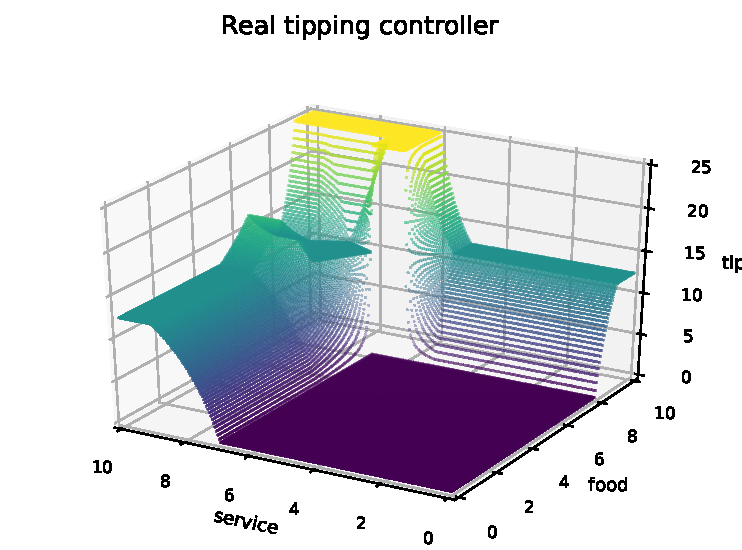
\includegraphics[width=.7\textwidth]{real-tip-controller-surface}
	\caption[Superficie de la función que modela el \acrlongsp{fcs} de ejemplo]{Las reglas y las particiones definen esta función. De ella obtendremos un conjunto de puntos aleatorio para comprobar si nuestra representación de \acrlongsp{fcs} como grafo computacional es capaz de ajustarse a ésta con la técnica del descenso del gradiente.}
	\label{fig:real-tip-controller-surface}
\end{figure}

Recogeremos una muestra aleatoria uniforme de $1500$ puntos de entre los $62500$ que conforman la representación de la superficie del controlador de ejemplo. Posteriormente se creará un controlador borroso y se entrenará aplicando el algoritmo de descenso del gradiente ADAM~\cite{kingma2014adam}.

El proceso de entrenamiento consistirá en la ejecución del algoritmo de propagación del error durante $2500$ epochs con una tasa de aprendizaje de $0.01$, la cual se ha considerado suficiente para el ejemplo en cuestión.

Durante el entrenamiento, las superficies evolucionan hacia una representación aproximada de lo que es el controlador original. En la Figura~\ref{fig:adjusted-tip-controller-training} podemos observar cómo evoluciona la superficie que representa el controlador ajustado.

\begin{figure}
	\centering
	\subfloat[Inicio]{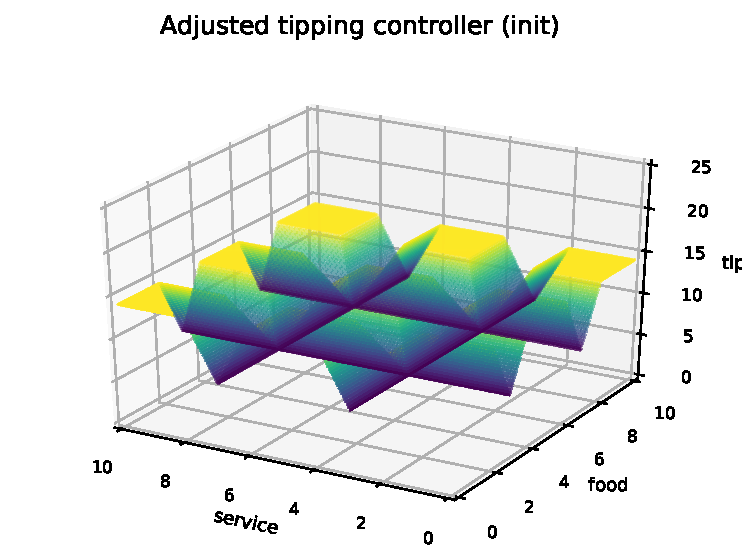
\includegraphics[width=.28\textwidth]{ajusted-tip-controller-at-init-training}}\qquad
	\subfloat[Epoch $250$]{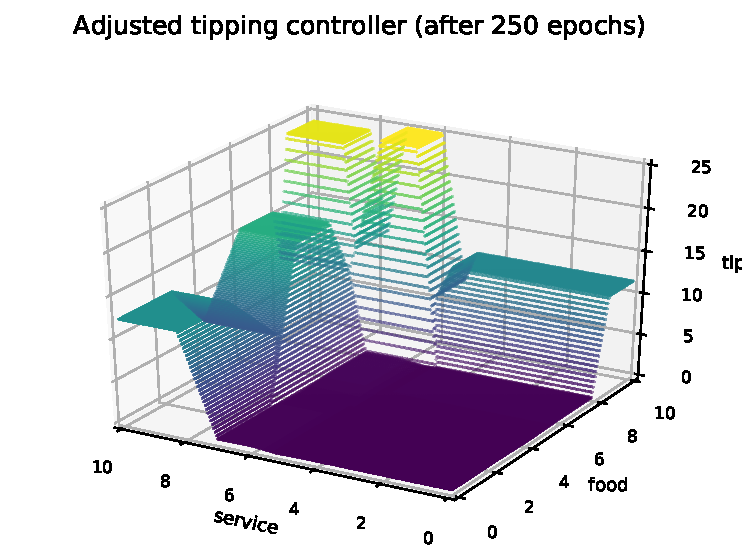
\includegraphics[width=.28\textwidth]{ajusted-tip-controller-at-half-training}}\qquad
	\subfloat[Epoch $500$]{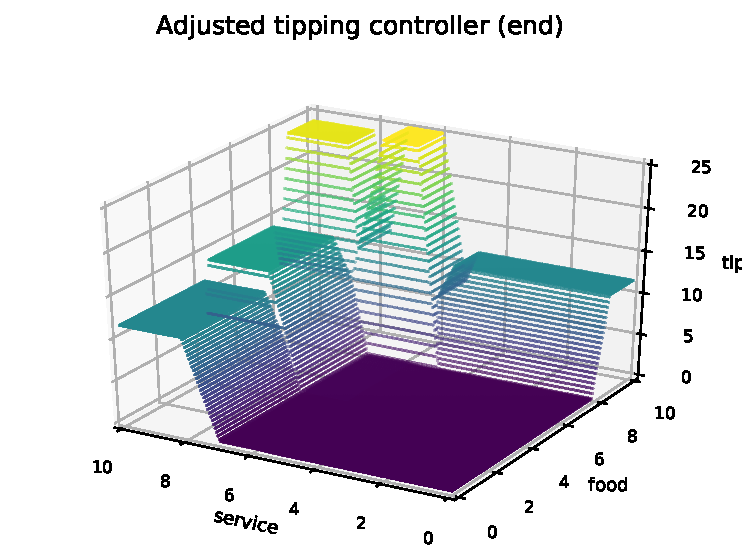
\includegraphics[width=.28\textwidth]{ajusted-tip-controller-at-end-training}}
	\caption[Evolución del \acrlongsp{fcs} de acuerdo al conjunto de datos extraido del ]{Particiones borrosas del \acrlongsp{fcs} de ajustado. Estas figuras muestran la superficie del controlador ajustado (a) al comienzo del proceso de entrenamiento, (b) tras $250$ iteraciones sobre el conjunto de entrenamiento y (c) al final del proceso del entrenamiento.}
	\label{fig:adjusted-tip-controller-training}
\end{figure}

Este proceso demuestra que es posible obtener \acrlongplsp{fcs}\index{sistema de control borroso} ajustados a un patrón de datos con un grado alto de precisión. La ventaja de este método radica en que es posible por tanto explicar mediante reglas el por qué de las predicciones que hace el modelo, a diferencia de otras técnicas como las \acrlongsp{ann}\index{red neuronal artificial}.

\section{Descripción de los datasets}

Del conjunto de datos descrito en la Tabla~\ref{tbl:main-variables} del capítulo~\nameref{ch:methodology} seleccionamos aquellos indicadores de interés: \textit{Distancia a líder}, \textit{Distancia a siguiente TLS}, \textit{Estado de siguiente TLS}, \textit{Velocidad}, \textit{Velocidad a líder} y \textit{Aceleración} (este último como salida a ajustar por el modelo). Estos valores conformarán los conjuntos de entrenamiento y de test tanto para cada uno de los sujetos $S_1$, $S_2$ y $S_3$, como para el conjunto global de éstos $S_A$.

Dado que nuestros modelos se basan en un esquema \textit{\idx{feed-forward}}, existe el inconveniente de que para ellos es imposible mantener una memoria del orden en el que se están sucediendo las entradas. Sin embargo, contamos con las derivadas de la posición respecto al líder (la aceleración y la velocidad al líder) y la velocidad, por lo que consideramos que disponemos de información temporal suficiente para este problema en concreto.

El resultado de la generación de los datasets de entrenamiento y test para todos los sujetos se resume en la Tabla~\ref{tbl:cf-datasets-description}

\section{Modelo basado en \acrlongplsp{fcs}\index{sistema de control borroso}}
\label{s:fcs-based-model}

\begin{table}[t]
	\centering
	\caption[Descripción de los conjuntos de datos]{Descripción de los conjuntos de datos para el entrenamiento de los modelos. $CF_{S_A}$ se corresponde con el modelo de conductor global, mientras que cada $CF_{S_i}$ es la porción de datos correspondiente al sujeto $S_i$.}
	\label{tbl:cf-datasets-description}
	\begin{tabularx}{\textwidth}{cYYYY}
		\toprule
		& & & \multicolumn{2}{c}{Tamaño} \\
		& Entradas & Salidas & Entrenamiento & Test \\
		\midrule
		\rowcolor{black!20} $CF_{S_1}$ & $7$ & $1$ & $1089$ & $543$ \\
		$CF_{S_2}$ & $7$ & $1$ & $1313$ & $560$ \\
		\rowcolor{black!20} $CF_{S_3}$ & $7$ & $1$ & $2067$ & $668$ \\
		$CF_{S_A}$ & $7$ & $1$ & $4469$ & $1771$ \\
		\bottomrule
	\end{tabularx}
\end{table}

Se han realizado entrenamientos sobre arquitecturas con diferente número de particiones borrosas en las variables. Las arquitecturas que se han considerado más relevantes (tras un proceso de ensayo y error) se describen en la Tabla~\ref{tbl:cf-fcs-architectures}. 

\begin{table*}
	\centering
	\caption[Resumen de las arquitecturas \ac{fcs}\index{sistema de control borroso} para el modelo longitudinal][2em]{Resumen de las arquitecturas seleccionadas. La posición de cada número de la arquitectura indica a qué variable lingüística se refiere (\textit{Distancia al líder}, \textit{Distancia a siguiente TLS}, \textit{TLS en verde}, \textit{TLS en amarillo}, \textit{TLS en rojo}, \textit{Velocidad} y \textit{Velocidad de aproximación al líder} respectivamente). Su valor se corresponde al número de conjuntos borrosos de la partición de cada una de ellas.}
	\label{tbl:cf-fcs-architectures}
	\begin{tabularx}{\linewidth}{cYYYYY}
		\toprule
		\multirow{2}{*}{} & \multirow{2}{*}{Arquitectura} & \multirow{2}{*}{Epochs} & \multicolumn{3}{c}{RMS}      \\ 
		& & & Entrenamiento & Validación & Test \\
		\midrule
		\rowcolor{black!20} $FCS_1$ & $2, 2, 2, 2, 2, 2, 2$ & $10^5$ & $0.059$ & $0.064$ & $0.062$  \\
		$FCS_2$ & $3, 3, 2, 2, 2, 3, 3$ & $10^5$ & $0.073$ & $0.079$ & $0.080$  \\
		\rowcolor{black!20} $FCS_3$ & $4, 3, 2, 2, 2, 3, 3$ & $10^5$ & $0.072$ & $0.078$ & $0.088$  \\
		$FCS_4$ & $5, 5, 2, 2, 2, 5, 5$ & $10^5$ & $0.063$ & $0.068$ & $0.109$  \\
		\bottomrule
	\end{tabularx}
\end{table*}

Todas las arquitecturas mantienen el número de conjuntos borrosos\index{conjunto borroso} asociados a las variables de estado del semáforo (verde, ámbar y rojo) a $2$. La razón es debido a que dicha variable sólo puede tomar dos valores, $0$ o $1$, y en la inicialización de sus respectivas particiones, estas variables ya toman dichos valores con un grado de pertenencia de $1$ en sus dominios.

Cada uno de los controladores se ha entrenado durante $250000$ \textit{epochs}\index{epoch}. En la Figura~\ref{fig:lm-fcs-rmse-all-comparisons} se puede observar la evolución en general y un detalle de la disminución del error durante el entrenamiento de los controladores. El error en test se ofrece a título informativo, y no ha sido usado para determinar las arquitecturas seleccionadas.

\begin{figure}
	\centering
	\subfloat[Entrenamiento y validación]{\includegraphics[width=.45\textwidth]{lm-fcs-rmse-all-training-and-validation-detail}}\qquad
	\subfloat[Test]{\includegraphics[width=.45\textwidth]{lm-fcs-rmse-all-test-detail}}
	\caption[Evolución del error durante el entrenamiento en las arquitecturas de \acrshort{fcs} para el modelo longitudinal]{Visión en detalle de la evolución del error en los conjuntos de entrenamiento y validación (izquierda) y de test (derecha). Para cada arquitectura, el color más transparente se corresponde al error en el conjunto de validación. El error de test se muestra debido a que nos ofrece puede ofrecer intuición de qué forma aprende la red, pero su evolución no se ha considerado para determinar las arquitecturas.}
	\label{fig:lm-fcs-rmse-all-comparisons}
\end{figure}

En un principio, el proceso de entrenamiento ha sido el habitual, ajustando todas las variables a la vez (particiones borrosas y reglas). Sin embargo, tras varias pruebas, se ha comprobado que el ajuste de las variables que determinan las particiones borrosas parece suceder más rápido que el ajuste de los pesos asociados a las reglas; por ello, en lugar entrenar a la vez, se ha particionado el entrenamiento en secuencias sucesivas de entrenamiento de reglas y entrenamiento de particiones borrosas.

Concretamente, los $250000$ epochs de entrenamiento han sido divididos en $250$ iteraciones de $800$ epochs ajustando sólo las reglas con una tasa de entrenamiento de $0.01$ seguidos de $200$ epochs ajustando sólo las variables de las particiones borrosas con una tasa de entrenamiento de $0.001$.

En este problema en concreto se ha observado que el entrenamiento realizado de esta manera hace que el \ac{rmse} descienda más rápido en el mismo número de iteraciones. Se puede observar que la arquitectura $FCS_1$ es la que mejor error en test ha alcanzado.

En las pruebas realizadas para el ajuste de controladores se ha observado además que los errores en entrenamiento y en test tienden a ser similares cuando los problemas son representables con un \acrlongsp{fcs}\index{sistema de control borroso}.

Éste será el modelo seleccionado para la comparativa final. Las funciones de pertenencia ajustadas se muestran en la Figura~\ref{fig:adjusted-fuzzy-partitions} contrastadas con las versiones del inicio del entrenamiento, donde $f_i$ se corresponde con la función de pertenencia del conjunto borroso $i$-ésimo de la variable.

\begin{figure}
	\centering
	\subfloat[Distancia a líder (\SI{0}{\meter} a \SI{50}{\meter} norm.)]{\includegraphics[width=.45\textwidth]{lm-fcs-best-architecture-leader-distance-variable-partition}}\qquad
	\subfloat[Distancia a siguiente semáforo  (\SI{0}{\meter} a \SI{100}{\meter} norm.)]{\includegraphics[width=.45\textwidth]{lm-fcs-best-architecture-next-tls-distance-variable-partition}}\qquad
	\subfloat[Velocidad (\SI{0}{\meter\per\second} a \SI{20}{\meter\per\second})]{\includegraphics[width=.45\textwidth]{lm-fcs-best-architecture-speed-variable-partition}}\qquad
	\subfloat[Velocidad a líder \SI{-40}{\meter\per\second} a \SI{40}{\meter\per\second})]{\includegraphics[width=.45\textwidth]{lm-fcs-best-architecture-speed-to-leader-variable-partition}}
	\caption[Particiones borrosas después de la operación de ajuste en el modelo longitudinal basado en \acrshort{fcs}]{Particiones borrosas después de la operación de ajuste en el modelo longitudinal basado en \acrshort{fcs}.}
	\label{fig:adjusted-fuzzy-partitions}
\end{figure}

Las funciones de pertenencia para el estado del semáforo no se incluyen ya que no se vieron modificadas en ningún entrenamiento. Después de todo, estas variables eran binarias, y las particiones borrosas se inicializan de tal manera que dichos valores siempre alcanzan un valor de pertenencia $1$. Las reglas son muy numerosas para ser incluidas en el texto, por lo que se han movido al apéndice \nameref{ch:derived-controller-rules} para no complicar en exceso el contenido del presente capítulo.

Un detalle que merece la pena destacar es el aprendizaje de la variable lingüística \textit{Velocidad a Líder}. En todos los entrenamientos con las arquitecturas de la Tabla~\ref{tbl:cf-fcs-architectures} el resultado ha sido un único conjunto difuso que cubre todo el dominio de la variable, con todas las reglas de activación teniendo dicho conjunto en cuenta. Esto da indicios de que dicha variable tiene un efecto mínimo o nulo sobre el comportamiento longitudinal, aunque esto contradice a prácticamente todos los modelos de la literatura consultados, por lo que la explicación no puede ser esa. La razón más plausible que podemos encontrar a dicho efecto es que, al tratarse de un entorno urbano, las velocidades que tratamos son muy bajas en comparación con las que se trabaja en este tipo de modelos, y por tanto, la diferencia de velocidades no son un factor determinante en comparación con el resto de variables.

En la Figura~\ref{fig:fcs-test-comparisons} se muestran los perfiles de la aceleración estimada por los controladores frente la aceleración real en cada momento. 

\begin{figure}
	\centering
	\subfloat[Perfil de aceleración]{\includegraphics[width=\textwidth]{lm-fcs-outs-all-test-comparison}}\qquad
	\subfloat[Detalle entre frames de $750$ a $1050$]{\includegraphics[width=\textwidth]{lm-fcs-outs-all-test-comparison-detail}}
	\caption[Comparación del perfil de aceleración real y el inferido por los modelos entrenados]{Comparación del perfil de aceleración real y el inferido por los modelos entrenados. En la visión general se puede observar el perfile real en color semi-transparente. Debajo, en el perfil, se amplía una pequeña sección del perfil para mostrar los diferentes ajustes de los modelos entrenados y cómo difieren del valor real.}
	\label{fig:fcs-test-comparisons}
\end{figure}

Se puede observar cómo se ajusta el controlador con menor error en test frente al resto. $FCS_1$ presenta picos que aproximan el valor inferido al valor real, mientras que el resto mantiene valores constantes.

\section{Modelo basado en \acrlongplsp{mlp}\index{perceptrón multicapa}}

Para determinar el modelo óptimo de \acrlongsp{mlp}\index{perceptrón multicapa}, se han realizado entrenamientos sobre arquitecturas con diferente cantidad de neuronas y capas ocultas. Las arquitecturas más ilustrativas de todas las probadas se resumen en la tabla~\ref{tbl:cf-mlp-architectures}.

\begin{table*}
	\centering
	\caption[Resumen de las arquitecturas de \acrlongplsp{mlp} para el modelo longitudinal][2em]{Resumen de las arquitecturas de de \acrlongplsp{mlp} para el modelo longitudinal. La posición de cada número de la topología indica el índice de la capa oculta y su valor el número de nodos (neuronas) que incluye dicha capa. Las arquitecturas seleccionadas en esta tabla son aquellas consideradas relevantes tras un proceso manual de ensayo y error.}
	\label{tbl:cf-mlp-architectures}
	\begin{tabularx}{\linewidth}{cYYYYY}
		\toprule
		\multirow{2}{*}{} & \multirow{2}{*}{Topología} & \multirow{2}{*}{Epochs} & \multicolumn{3}{c}{RMS} \\
		& & & Entrenamiento & Validación & Test \\
		\midrule
		\rowcolor{black!20} $MLP_1$ & $16$        & $10^5$ & $0.057$ & $0.057$ & $0.069$  \\
		$MLP_2$ & $8, 2$      & $10^5$ & $0.061$ & $0.061$ & $0.056$  \\
		\rowcolor{black!20} $MLP_3$ & $16, 8$     & $10^5$ & $0.051$ & $0.051$ & $0.060$  \\
		$MLP_4$ & $16, 16, 8$ & $10^5$ & $0.046$ & $0.046$ & $0.061$  \\
		\bottomrule
	\end{tabularx}
\end{table*}

El modelo de funciones de activación que se ha utilizado es de tipo tangente hiperbólica en todas las neuronas salvo en la última, que se ha utilizado una activación lineal.

En pruebas previas a la selección de estas funciones de activación se han utilizado también funciones de activación de tipo \acrshort{relu}\index{ReLU}, pero las tasas de error tras el entrenamiento eran notablemente más altas por lo que se ha optado al final por el uso de activación basada en tangente hiperbólica. Los pesos de la red han sido inicializados con una muestra aleatoria uniforme de valores reales en el intervalo $(-0.25, 0.25)$.

La Figura~\ref{fig:lm-mlp-rmse-all-comparisons} muestra la evolución del \gls{rmse} durante el proceso de entrenamiento. También se ilustra el error de test, aunque éste no se ha utilizado para decidir las arquitecturas.

\begin{figure}
	\centering
	\subfloat[Entrenamiento y validación]{\includegraphics[width=.45\textwidth]{lm-mlp-rmse-all-training-and-validation-detail}}\qquad
	\subfloat[Test]{\includegraphics[width=.45\textwidth]{lm-mlp-rmse-all-test-detail}}
	\caption[Evolución del error durante el entrenamiento en las arquitecturas de \acrshort{mlp} para el modelo longitudinal]{Visión en detalle de la evolución del error en los conjuntos de entrenamiento y validación (izquierda) y de test (derecha). Para cada arquitectura, el color más transparente se corresponde al error en el conjunto de validación. El error de test se muestra debido a que nos ofrece puede ofrecer intuición de qué forma aprende la red, pero su evolución no se ha considerado para determinar las arquitecturas.}
	\label{fig:lm-mlp-rmse-all-comparisons}
\end{figure}

Estos errores se encuentran entre los \SI{0.05}{\metre\per\square\second} y los \SI{0.07}{\metre\per\square\second}, lo cual consideramos que es una aproximación aceptable. Una particularidad del problema ha sido la inestabilidad de los entrenamientos, esto es, la alta sensibilidad a los valores de inicialización de los parámetros. La intuición tras observar cómo evolucionan los entrenamientos es que la función de error sufre de muchos mínimos locales o mesetas.

Una visión de detalle del ajuste de estas arquitecturas al conjunto de test se observa en la Figura~\ref{fig:cf-mlp-test-comparisons}, con el perfil de aceleración del conjunto de test y los perfiles de aceleración de las redes entrenadas.

\begin{figure}
	\centering
	\subfloat[Perfil completo]{\includegraphics[width=\textwidth]{lm-mlp-outs-all-test-comparison}}\qquad
	\subfloat[Detalle entre frames de $750$ a $1050$]{\includegraphics[width=\textwidth]{lm-mlp-outs-all-test-comparison-detail}}
	\caption[Comparación del perfil de aceleración real y el inferido por los modelos entrenados]{Comparación del perfil de aceleración real y el inferido por los modelos entrenados. En la visión general se puede observar el perfil real en semi-transparente. En el detalle, se amplía una pequeña sección del perfil para mostrar los diferentes ajustes de los modelos entrenados y cómo difieren del valor real.}
	\label{fig:cf-mlp-test-comparisons}
\end{figure}

Al contrastar los errores de test, podemos determinar que la arquitectura que mejor generaliza es la $MLP_2$, hecho que se confirma en el ajuste de los perfiles de aceleración. Por lo tanto, parece razonable elegir el modelo $MLP_2$ como candidato para la representación del modelo longitudinal de los conductores.

\section{Comparación entre modelos}

Las mejores arquitecturas de ambos modelos han sido la $MLP_2$ para los \acrlongplsp{mlp}\index{perceptrón multicapa} y $FCS_1$ para los \acrlongplsp{fcs}\index{sistema de control borroso}. Los errores y el perfil de aceleración para ambos modelos se muestran en la Figura~\ref{fig:cf-comparison-between-best-mlp-and-fcs-architecture}.

\begin{figure}
	\centering
	\subfloat[Error en test]{\includegraphics[width=.46\textwidth]{comparison-between-best-mlp-and-fcs-architecture-rms}}\qquad
	\subfloat[Perfil de aceleración]{\includegraphics[width=.46\textwidth]{comparison-between-best-mlp-and-fcs-architecture-acceleration-profile}}
	\caption[Comparación entre los dos tipos de modelo longitudinal]{Comparación de la mejor arquitectura de \acrlongplsp{mlp} frente a la mejor arquitectura de \acrlongplsp{fcs}: (a) diferencia entre los errores cuadráticos medios de ambas arquitecturas y (b) perfiles de aceleración en el conjunto de test.}
	\label{fig:cf-comparison-between-best-mlp-and-fcs-architecture}
\end{figure}

Aunque el modelo arroja un error bajo en test, y además tiende a ajustarse al perfil de aceleración, parece que el problema es suficientemente complejo como para no poder representarse como un simple \acrlongsp{fcs}\index{sistema de control borroso}. Además, el error arrojado por el \acrlongsp{mlp}\index{perceptrón multicapa} es sustancialmente menor.

Los resultados sugieren por tanto que la arquitectura elegida para el modelo longitudinal será la $MLP_2$.

\section{Modelos longitudinales específicos}

La arquitectura seleccionada ha sido usada para generar los modelos de cada uno de los conductores por separado para comprobar que (i) los errores y precisiones se mantienen en el orden del modelo global, y (ii) capturan las particularidades de cada sujeto de estudio.

En la Figura~\ref{fig:lm-specific-training-validation-and-test-comparison} se muestra la evolución del \gls{rmse}\index{RMSE} en test para cada uno de los sujetos tras entrenar los modelos de arquitectura $MLP_2$ con los datos de los sujetos.

\begin{figure}
	\centering
	\includegraphics[width=\textwidth]{lm-specific-rmse-all-test-detail}
	\caption[Comparativa de la evolución del \gls{rmse} en test para los sujetos de la arquitectura seleccionada para el modelo longitudinal]{Comparativa de la evolución del error de test entre los sujetos de la arquitectura seleccionada para el modelo longitudinal. El \gls{rmse} en test en el caso del sujeto $S_2$ es muy alto (mayor que $0.2$) comparado con el error en el resto de sujetos y en el global.}
	\label{fig:lm-specific-training-validation-and-test-comparison}
\end{figure}

Se puede observar que el error en test de los sujetos es ligeramente mayor que el del conjunto global. Esto se puede explicar por la mayor capacidad de generalización de $S_A$ al haber sido entrenado con un conjunto de datos mayor. Los errores se resumen en la Tabla~\ref{tbl:lm-specific-rmse}.

\begin{table}
	\centering
	\caption[Resumen de los valores de \Acrshort{rmse} para los modelos específicos de comportamiento longitudinal]{Resumen de los valores de \Acrshort{rmse} para los modelos específicos de comportamiento longitudinal.}
	\label{tbl:lm-specific-rmse}
	\begin{tabularx}{\linewidth}{cYYYYY}
		\toprule
		\multirow{2}{*}{} & \multicolumn{3}{c}{\ac{rmse}}      \\ 
		& Entrenamiento & Validación & Test \\
		\midrule
		\rowcolor{black!20} $S_A$ & $0.056$ & $0.062$ & $0.057$  \\
		$S_1$ & $0.045$ & $0.039$ & $0.060$  \\
		\rowcolor{black!20} $S_2$ & $0.048$ & $0.047$ & $0.058$  \\
		$S_3$ & $0.055$ & $0.054$ & $0.058$  \\
		\bottomrule
	\end{tabularx}
\end{table}

Los resultados parecen sugerir que los errores específicos se mantienen aproximadamente dentro del mismo rango de error que el modelo global. Para verificar que esta topología es capaz de capturar las diferencias entre conductores, comparamos los perfiles de aceleración de los conductores en la Figura~\ref{fig:lm-subjects-comparison}.

En ella se muestra cada perfil de modelo sobre cada uno de los perfiles reales. Podemos observar que, para cada perfil de aceleración, los más similares son los de sus respectivos modelos. En la Tabla~\ref{tbl:lm-subjects-comparison} se describen los \gls{rmse}\index{RMSE} cruzados para de cada uno de los conductores.

\begin{figure}[t]
	\centering
	\subfloat[Sujeto $S_1$]{\includegraphics[width=\textwidth]{lm-subjects-comparison-with-edgar-acceleration-profiles}}\qquad
	\subfloat[Sujeto $S_2$]{\includegraphics[width=\textwidth]{lm-subjects-comparison-with-jj-acceleration-profiles}}\qquad
	\subfloat[Sujeto $S_3$]{\includegraphics[width=\textwidth]{lm-subjects-comparison-with-miguel-acceleration-profiles}}
	\caption[Diferencia entre los perfiles de aceleración para los diferentes sujetos]{Diferencia entre los perfiles de aceleración para los diferentes sujetos.}
	\label{fig:lm-subjects-comparison}
\end{figure}

\begin{table}
	\centering
	\caption[Comparación de los errores de aceleración en los diferentes modelos longitudinales]{Comparación de los errores de aceleración en los diferentes modelos longitudinales. Las filas se corresponden con los recorridos mientras que las columnas se corresponden con los modelos que se han intentado ajustar a ellas.}
	\label{tbl:lm-subjects-comparison}
	\begin{tabularx}{\linewidth}{YYYY}
		\toprule
		& $S_1$ & $S_2$ & $S_3$ \\
		\midrule
		\rowcolor{black!20} $S_1$ & $0.059$        & $0.074$        & $0.070$ \\
		$S_2$ & $0.064$        & $0.058$        & $0.067$ \\
		\rowcolor{black!20} $S_3$ & $0.065$        & $0.065$        & $0.057$ \\
		\bottomrule
	\end{tabularx}
\end{table}

Se observa que el \gls{rmse}\index{RMSE} es menor cuando el modelo de conductor se aplica sobre los datos del conjunto de test de sus respectivos conductores. Estos modelos basados en la arquitectura $MLP_2$ serán los comportamientos longitudinales de los sujetos en el simulador. Veremos su desempeño en el capítulo \nameref{ch:simulation-implementation}.
\chapter{Comportamiento de cambio de carril}
\label{ch:lane-change-model}

El problema del cambio de carril determina cuándo y cómo realiza los cambios de carril un conductor en un momento determinado. A priori la intuición sobre el problema es que muchos de los factores determinantes no son medibles en el mundo real y/o en el entorno simulado (e.g. estados de humor, condición física, eventos fortuitos, etcétera).

En un trabajo anterior\cite{CITA DEL ARTÍCULO DE LANE EXECUTION CUANDO NOS LO PUBLIQUEN} se trataron de controlar muchos de estos factores dividiendo el problema en dos partes, la intención de cambio y la ejecución del cambio, fijando el primero de manera que los conductores sólo cambiaban de carril cuando se les ordenaba y permitiendo estudiar, de esta manera, cómo diferentes perfiles de conductores ejecutan de diferente forma el cambio de carril y cómo este fenómenos es modelable.

En este trabajo se tratará de modelar sin embargo el proceso de cambio de carril como un todo, esto es, decidir en cada momento si cambiar a un caril (i.e. izquierda o derecha) o no hacerlo, a partir de las variables medibles del entorno real y simulado.

El problema de ajuste será por tanto un problema de clasificación donde se tratará de maximizar el número de aciertos entre los cambios de carril realizados y el modelo a ajustar. La figura~\ref{fig:lc-lane-change-profiles}.

\begin{figure}
	\centering
	\subfloat[]{\includegraphics[width=.45\textwidth]{lc-lane-change-hist-training}}\qquad
	\subfloat[]{\includegraphics[width=.45\textwidth]{lc-lane-change-hist-test}}
	\caption[Perfiles de cambios de carril en los conjuntos de entrenamiento y test]{Perfiles de cambio de carril en los conjuntos de entrenamiento y de cambios de carril en el conjunto de test. }
	\label{fig:lc-lane-change-profiles}
\end{figure}

Las técnicas que se han seleccionado para tratar el cambio de carril son las siguientes:

\begin{enumerate}
	\item \ac{mlp}. Los \acp{mlp}, más ahora en la época del \textit{deep-learning} son una de las técnicas más usadas para problemas de clasificación. En esta época del \textit{deep-learning} han aumentado su eficiencia varios ordenes de magnitud en capacidad de aprendizaje y, por tanto, en rendimiento a la hora de clasificar.
	\item \ac{cnn}. Otro de los grandes exponentes a la hora de clasificar, sobre todo trabajando con mapas de características $n$-dimensionales con las \acp{cnn}. Al representar la evolución temporal del entorno circundante como un espacio tridimensional, podemos aplicar esta técnica para la identificación de características de manera, supuestamente, más eficiente.
\end{enumerate}

Ambos modelos, al igual que ocurría con el modelo longitudinal, han sido entrenados ajustando sus parámetros con el algoritmo ADAM~\cite{kingma2014adam}. Las funciones de activación, sin embargo, varían, y por tanto la inicialización de las variables también\sidenote{La inicialización clásica, de valores uniformes en un intervalo pequeño alrededor de 0 haría que la mitad de los valores cayesen por debajo de 0. Si la neurona tiene una función de activación de tipo \ac{relu}, el peso no se vería modificado, ya que su derivada será siempre 0}.

En este caso, ambos modelos hacen uso de neuronas de activación de tipo \ac{relu}, salvo en la última capa que la activación es lineal. Para inicializar los pesos de las variables se hace uso del algoritmo Glorot~\cite{glorot2010understanding} (también denominado Xavier) debido a su mejor desempeño, sobre todo en redes con funciones de activación tipo \ac{relu}~\cite{glorot2011deep}\sidenote{Esta inicialización se basa en intentar mantener la misma desviación típica de gradientes en cada capa de la red. En~\cite{glorot2010understanding} determinan que ésta debe ser $\sigma^l = \frac{2}{\mathbf{card}(W^l_{in}) + \mathbf{card}(W^l_{out})}$, siendo $\mathbf{card}(W^l_{in})$ y $\mathbf{card}(W^l_{out})$ el número de entradas y de salidas de la capa, extrayendo posteriormente sus valores de una distribución aleatoria de la forma $X^l \sim \mathcal{N}(\mu=0,\sigma=\sigma^l)$}.

Al tratarse además de un problema de clasificación donde las clases son mutuamente excluyentes, a la capa de salida de las redes se le ha aplicado una normalización\sidenote{
	La normalización usada ha sido la operación denominada softmax, definida como:
	
	\begin{equation}
		softmax(\vec{x})_i = \frac{e^{x_i}}{\sum_{j=1}^n e^{x_j}}
		\label{eq:softmax}
	\end{equation}
} para transformar el vector de salida en un vector de probabilidades, siendo el cambio de carril seleccionado la salida con el valor de probabilidad más alto.

Antes de pasar a la descripción de los modelos, queda hablar del sesgo existente en los datos de entrenamiento. Debido a la naturaleza el problema, el número de ejemplos existentes de cambios de carril es significativamente menor al existente de no cambios de carril. Este sesgo hace que los modelos se entrenen rápidamente para marcar todos los ejemplos como \enquote{no cambio}, dificultando el ajuste posterior hacia cambios a izquierda o derecha.

Por tanto, debido a que (i) las limitaciones de la máquina no nos permiten operar con los conjuntos completos en cada epoch y (ii) existe un sesgo hacia predicciones de \enquote{no cambio}, en cada uno de los epochs, se usará un batch para entrenar de tamaño $m$ compuesto por una selección aleatoria de todos los ejemplos equidistribuida entre las clases de los ejemplos (esto es, aproximadamente $\frac{m}{3}$ para cada clase \enquote{cambio izda.}, \enquote{no cambio} y \enquote{cambio dcha.}).

\section{Modelo \ac{mlp}}

Los entrenamientos han sido realizados sobre diferentes topologías, siendo las más representativas las descritas en la tabla~~\ref{tbl:lc-mlp-architectures}.

\begin{table}
	\caption[Resumen de las arquitecturas \ac{mlp} para el modelo de cambio de carril]{Resumen de las arquitecturas de \ac{mlp} para el modelo de cambio de carril. La posición de cada número de la topología indica la capa, siendo su valor el número de nodos (neuronas) que incluye dicha capa. Las arquitecturas seleccionadas en esta tabla son aquellas consideradas relevantes tras un proceso manual de ensayo y error.}
	\label{tbl:cf-mlp-architectures}
	\begin{tabular}{cccccccccc}
		\hline
		\multirow{2}{*}{Nombre} & \multirow{2}{*}{Topología} & \multirow{2}{*}{Epochs} & \multirow{2}{*}{Dropout} & \multicolumn{3}{c}{Precisión} & \multicolumn{3}{c}{Loss}      \\
		& & & & Training & Validation & Test & Training & Validation & Test \\ \hline
		$MLP_1$ & $X, X, X$ & $10^5$ & $0.1$ & $0.XXX$ & $0.XXX$ & $0.XXX$ & $0.XXX$ & $0.XXX$ & $0.XXX$ \\
		$MLP_2$ & $X, X, X$ & $10^5$ & $0.1$ & $0.XXX$ & $0.XXX$ & $0.XXX$ & $0.XXX$ & $0.XXX$ & $0.XXX$ \\
		$MLP_3$ & $X, X, X$ & $10^5$ & $0.1$ & $0.XXX$ & $0.XXX$ & $0.XXX$ & $0.XXX$ & $0.XXX$ & $0.XXX$ \\
		$MLP_4$ & $X, X, X$ & $10^5$ & $0.1$ & $0.XXX$ & $0.XXX$ & $0.XXX$ & $0.XXX$ & $0.XXX$ & $0.XXX$ \\ \hline
	\end{tabular}
\end{table}

Se han entrenado más redes, pero no se han incluido al no aportar información relevante en la descripción del proceso de entrenamiento.

Cada una de las redes se ha entrenado durante $XXX$ epochs. Debido a las limitaciones de memoria RAM en la máquina de entrenamiento, los epochs no incluyen todo el conjunto de entrenamiento en cada pasada, sino que se limitan a \textit{batches} de $YYY$ elementos seleccionados aleatoriamente del conjunto total de datos.

. En la Figura~\ref{fig:adjusted-fcs} se puede observar la evolución en general y un detalle de la disminución del error en test de los controladores.

\begin{figure}
	\centering
	\subfloat[]{\includegraphics[width=.45\textwidth]{fcs-all-test}}\qquad
	\subfloat[]{\includegraphics[width=.45\textwidth]{fcs-all-test-detail}}
	\caption[Evolución del error en test de los controladores difusos ajustados]{Visión general y detalle de la evolución del error en test de los diferentes controladores difusos ajustados.}
	\label{fig:adjusted-fcs}
\end{figure}

El proceso de entrenamiento seguido no ha sido el del ajuste de todas las variables en su conjunto. La razón principal de esto es que el ajuste de las variables que determinan las particiones difusas parece suceder órdenes de magnitud más rápido que el ajuste de los pesos asociados a las reglas.

Por tanto, y para este problema en concreto, El entrenamiento se realiza iterativamente alternando conjuntos de epochs dedicados a las reglas y conjuntos de epochs dedicados a las variables de las reglas difusas.

En lugar de eso se ha particionado el entrenamiento en secuencias sucesivas de entrenamiento de reglas y entrenamiento de particiones difusas. Concretamente, los $250.000$ epochs de entrenamiento se corresponden a $250$ iteraciones de $800$ epochs ajustando sólo las reglas seguidos de $200$ epochs ajustando las variables de las particiones difusas.

Empíricamente (y en este problema en concreto) se ha podido observar que el entrenamiento realizado de esta manera hace que el \ac{rmse} descienda más rápido en el mismo número de iteraciones.

Tras el entrenamiento, el controlador difuso que menor error en test arroja es el $FCS_2$\sidenote{
	Para el controlador $FCS_2$, la forma de sus particiones difusas queda, para las variables binarias sin apenas ajuste:
	\includegraphics{fcs-best-architecture-next-tls-green-yellow-and-red-variable-partition}
	El resto de particiones sí se han visto modificadas:
	\includegraphics{fcs-best-architecture-leader-distance-variable-partition}
	\includegraphics{fcs-best-architecture-next-tls-distance-variable-partition}
	\includegraphics{fcs-best-architecture-speed-variable-partition}
	\includegraphics{fcs-best-architecture-speed-to-leader-variable-partition}
	En transparente se puede ver el estado inicial de la partición, y en opaco la forma de ésta tras el proceso de entrenamiento.
}. Por tanto, éste será el modelo seleccionado para la comparativa final.


\section{Modelo \ac{cnn}}

\TODO{Indicar que, en este modelo concreto, las imágenes de los deepmap se han modificado dinámicamente en el proceso de alimentación de la red de tal manera que los extremos derecho e izquierdo de éstas se corresponden con los bordes izquierdo y derecho respectivamente para mantener la coherencia espacial en la horizontal.}

\TODO{Indicar que a la red de convolucion se la alimenta con todos los datos, pero que las convoluciones se realizan únicamente con imágenes, y el resto de arámetros se introducen en la fase de inferencia}

Para determinar el modelo óptimo de \ac{mlp} en comportamiento longitudinal, se han realizado entrenamientos sobre arquitecturas con diferente cantidad de neuronas y capas ocultas. Las arquitecturas más ilustrativas de todas las probadas se resumen en la tabla~\ref{tbl:cf-mlp-architectures}.

\begin{table*}
	\caption[Resumen de las arquitecturas \ac{mlp} para el modelo longitudinal]{Resumen de las arquitecturas de \ac{mlp} para el modelo longitudinal. La posición de cada número de la topología indica la capa, siendo su valor el número de nodos (neuronas) que incluye dicha capa. Las arquitecturas seleccionadas en esta tabla son aquellas consideradas relevantes tras un proceso manual de ensayo y error.}
	\label{tbl:cf-mlp-architectures}
	\begin{tabular}{ccccccc}
		\hline
		\multirow{2}{*}{Nombre} & \multirow{2}{*}{Topología} & \multirow{2}{*}{Epochs} & \multirow{2}{*}{Dropout} & \multicolumn{3}{c}{RMS}      \\
		&                            &                         &                          & Training & Validation & Test \\ \hline
		$MLP_1$ & $7, 16, 1$                 & $10^5$                  & $0.1$                    & $0.052741$      & $0.057301$        & $0.059253$  \\
		$MLP_2$ & $7, 8, 4, 1$               & $10^5$                  & $0.1$                    & $0.056341$      & $0.061951$        & $0.056607$  \\
		$MLP_3$ & $7, 16, 8, 1$              & $10^5$                  & $0.1$                    & $0.046404$      & $0.051878$        & $0.059681$  \\
		$MLP_4$ & $7, 16, 16, 8, 1$          & $10^5$                  & $0.1$                    & $0.042789$      & $0.046876$        & $0.060971$  \\ \hline
	\end{tabular}
\end{table*}

El modelo de neuronas de activación que se ha utilizado es de tipo tangente hiperbólica en todas las neuronas salvo en la última, que se ha utilizado una activación lineal en todas las neuronas salvo en la neurona de salida que se ha utilizado una activación lineal\sidenote{Se han utilizado también funciones de activación de tipo \ac{relu}, pero las tasas de error tras el entrenamiento eran notablemente más altas por lo que se ha optado al final por el uso de activación basada en tangente hiperbólica.}. Los pesos de la red han sido inicializados con una muestra aleatoria uniforme de valores reales en el intervalo $(-0.25, 0.25)$.

El error que se trata de minimizar es el error cuadrático medio entre los valores de aceleración del conjunto reales y los ajustados por el modelo. La Figura~\ref{fig:rms-all-in-training-and-validation-mlp-detail} muestra la evolución de este error durante el proceso de entrenamiento.

\begin{figure}
	\centering
	\includegraphics{rms-all-in-training-and-validation-mlp-detail}
	\caption[Evolución del error en entrenamiento en los \ac{mlp} para las arquitecturas seleccionadas]{Visión en detalle de la evolución del error en los conjuntos de entrenamiento y validación. Para cada arquitectura, el color más transparente se corresponde al error en el conjunto de validación..}
	\label{fig:rms-all-in-training-and-validation-mlp-detail}
\end{figure}

Estos errores se encuentran entre los \SI{0.05}{\metre\per\square\second} y los \SI{0.07}{\metre\per\square\second}, lo cual consideramos que es una aproximación aceptable. Una particularidad del problema ha sido la inestabilidad de los entrenamientos, esto es, la alta sensibilidad a los valores de inicialización de los parámetros. La intuición tras ver la evolución de los entrenamientos es que la función de error del problema tiene muchos mínimos locales o mesetas.

Al contrastar los errores de test, podemos determinar que la arquitectura que parece que mejor generaliza es la $MLP_2$ (arquitectura $7, 8, 2, 1$), como podemos ver en la figura~\ref{fig:rms-all-test-mlp-detail}.

\begin{figure}
	\centering
	\includegraphics{rms-all-test-mlp-detail}
	\caption[Evolución del error en el conjunto de test durante el entrenamiento]{Visión en detalle de la evolución del error en el conjunto de test. Aunque no se ha considerado para determinar las arquitecturas, sí se ha recogido la información de la evolución del error en el conjunto de test debido a que nos ofrece puede ofrecer intuición de qué forma aprende la red. Por lo que podemos observar, para el problema en cuestión las redes más potentes tienden a sobre-entrenarse.}
	\label{fig:rms-all-test-mlp-detail}
\end{figure}

Una visión de detalle del ajuste de estas arquitecturas al conjunto de test se puede ver en la figura~\ref{fig:mlp-test-comparisons}, donde se muestra el perfil de aceleración del conjunto de test y los perfiles de aceleración de las redes entrenadas.

\begin{figure}
	\centering
	\subfloat[]{\includegraphics[width=.45\textwidth]{mlp-test-comparison}}\qquad
	\subfloat[]{\includegraphics[width=.45\textwidth]{mlp-test-comparison-detail}}
	\caption[Comparación del perfil de aceleración real y el inferido por los modelos entrenados]{Comparación del perfil de aceleración real y el inferido por los modelos entrenados. En la visión general se puede observar, en transparente, el perfil real. A la derecha se amplía una pequeña sección del perfil para mostrar los diferentes ajustes de los modelos entrenados y cómo difieren del valor real.}
	\label{fig:mlp-test-comparisons}
\end{figure}

A la vista de los resultados, y dado que las arquitecturas se ajustan razonablemente bien, es razonable elegir el modelo $MLP_2$ debido a que es el que aparentemente mejor generaliza los comportamientos del conjunto de conductores.

\section{Comparación entre modelos}

Las mejores arquitecturas de ambos modelos han sido la $MLP_2$ para los \acp{mlp} y $FCS_x$ para los \acp{fcs}. Los errores y el perfil de aceleración para ambos modelos se muestran en la figura~\ref{fig:comparison-between-best-mlp-and-fcs-architecture}.

\begin{figure}
	\centering
	\subfloat[]{\includegraphics[width=.46\textwidth]{comparison-between-best-mlp-and-fcs-architecture-rms}}\qquad
	\subfloat[]{\includegraphics[width=.46\textwidth]{comparison-between-best-mlp-and-fcs-architecture-acceleration-profile}}
	\caption[Comparación entre los dos tipos de modelo longitudinal]{Comparación de la mejor arquitectura \ac{mlp} frente a la mejor arquitectura \ac{fcs}: (a) diferencia entre los errores cuadráticos medios de ambas arquitecturas y (b) perfiles de aceleración en el conjunto de test.}
	\label{fig:comparison-between-best-mlp-and-fcs-architecture}
\end{figure}

Aunque el modelo basado en \ac{fcs} arroja un error bajo en test y parece que tiende a ajustarse al perfil de aceleración, parece que el problema es suficientemente complejo como para no poder representarse como un simple controlador difuso.

Además, el error arrojado por el \ac{mlp} es sustancialmente menor y, por tanto, la arquitectura elegida para el modelo longitudinal será el \ac{mlp} $MLP_2$.
\chapter{Modelos específicos de conductores}
\label{ch:specific-models}

En los capítulos anteriores se han decidido los modelos candidatos que conformarán el modelo de comportamiento de conductor general.

Ahora que sabemos cuáles son las técnicas y arquitecturas que mejor se adecuan a este problema con los datos que disponemos, pasaremos a probarlas con los datos de los conductores específicos, comprobando si:

\begin{itemize}
	\item Los errores y precisiones se mantienen en el orden del modelo global.
	\item Los modelos capturan las particularidades de cada sujeto de estudio.
\end{itemize}

Para ello, compararemos primero el modelo longitudinal global con los modelos entrenados de los sujetos. Posteriormente, compararemos los modelos de los sujetos contra los conjuntos de test de cada uno de ellos.

\section{Modelo longitudinal}

La arquitectura que se ha entrenado para cada uno de los sujetos ha sido la $MLP_2$ (topología $7, 8, 4, 1$). En la Figura~\ref{fig:lm-specific-training-validation-and-test-comparison} 

\begin{figure}[!b]
	\centering
	\includegraphics[width=\textwidth]{lm-specific-rmse-all-test-detail}
	\caption[Comparativa de la evolución del \gls{rmse} en test para los sujetos de la arquitectura seleccionada para el modelo longitudinal]{Comparativa de la evolución del error de test entre los sujetos de la arquitectura seleccionada para el modelo longitudinal. El \gls{rmse} en test en el caso del sujeto $S_2$ es muy alto (mayor que $0.2$) comparado con el error en el resto de sujetos y en el global.}
	\label{fig:lm-specific-training-validation-and-test-comparison}
\end{figure}

Se puede observar que el error en test de los sujetos es ligeramente mayor que el del conjunto global. Esto se puede explicar por la mayor capacidad de generalización de $S_A$ al haber sido entrenado con un conjunto de datos mayor.

\begin{table}
	\centering
	\caption[Resumen de los valores de \gls{rmse} para los modelos específicos de comportamiento longitudinal]{Resumen de los valores de \gls{rmse} para los modelos específicos de comportamiento longitudinal.}
	\label{tbl:lm-specific-rmse}
	\begin{tabular}{cccccc}
		\toprule
		\multirow{2}{*}{} & \multicolumn{3}{c}{\ac{rmse}}      \\ 
		& Entrenamiento & Validación & Test \\
		\midrule
		\rowcolor{black!20} $S_A$ & $0.056$ & $0.062$ & $0.057$  \\
		$S_1$ & $0.045$ & $0.039$ & $0.060$  \\
		\rowcolor{black!20} $S_2$ & $0.048$ & $0.047$ & $0.058$  \\
		$S_3$ & $0.055$ & $0.054$ & $0.058$  \\
		\bottomrule
	\end{tabular}
\end{table}

\section{Cambio de carril}

En el caso del modelo de cambio de carril, la arquitectura con la que se han entrenado los modelos específicos es al $CNN_1$ (topología $c16$-$4$-$18$-$v$, $d128$). En la Figura~\ref{fig:lc-specific-rmse-all-test-detail} 

\begin{figure}
	\centering
	\includegraphics[width=\textwidth]{lc-specific-rmse-all-test-detail}
	\caption[\acrshort{rmse} en test entre los sujetos de la arquitectura seleccionada para el modelo de cambio de carril]{Comparativa de la evolución del error de test entre los sujetos de la arquitectura seleccionada para el modelo de cambio de carril.}
	\label{fig:lc-specific-rmse-all-test-detail}
\end{figure}

La precisión alcanzada en los modelos específicos entrenados con esta arquitectura es mayor que la alcanzada por el modelo global. Tiene sentido ya que el modelo global se ha entrenado con el conjunto de datos global y por tanto no obedece exactamente al comportamiento de ningún perfil en concreto, mientras que en los modelos específicos sí. En la tabla~\ref{tbl:lc-specific-accuracy} se exponen los valores de la precisión de este modelo.

\begin{table}
	\centering
	\caption[Precisión alcanzada para los modelos específicos de cambio de carril]{Resumen de los valores de precisión para los modelos específicos de cambio de carril.}
	\label{tbl:lc-specific-accuracy}
	\begin{tabular}{cccccc}
		\toprule
		\multirow{2}{*}{} & \multicolumn{3}{c}{\ac{rmse}}      \\ 
		& Entrenamiento & Validación & Test \\
		\midrule
		\rowcolor{black!20} $S_A$ & $0.588$ & $0.576$ & $0.573$  \\
		$S_1$ & $0.805$ & $0.763$ & $0.768$  \\
		\rowcolor{black!20} $S_2$ & $0.683$ & $0.708$ & $0.706$  \\
		$S_3$ & $0.727$ & $0.706$ & $0.710$  \\
		\bottomrule
	\end{tabular}
\end{table}


\section{Personalización en modelos de conducción específicos}

Las anteriores secciones han mostrado cómo las topologías seleccionadas en los capítulos \nameref{ch:longitudinal-model} y \nameref{ch:lane-change-model} son adecuadas para modelar los comportamientos específicos de cada conductor, además de el conjunto global.

Lo interesante es comprobar si estas topologías son capaces de capturar las diferencias entre conductores. Para ello, comprobaremos cómo se comportan cada uno de los conductores en todos los conjuntos de test.

En el caso del modelo longitudinal, los valores de error cruzados entre sujetos se muestran en la tabla~\ref{tbl:lm-subjects-comparison}.

\begin{figure}[t]
	\centering
	\subfloat[Sujeto $S_1$]{\includegraphics[width=\textwidth]{lm-subjects-comparison-with-edgar-acceleration-profiles}}\qquad
	\subfloat[Sujeto $S_2$]{\includegraphics[width=\textwidth]{lm-subjects-comparison-with-jj-acceleration-profiles}}\qquad
	\subfloat[Sujeto $S_3$]{\includegraphics[width=\textwidth]{lm-subjects-comparison-with-miguel-acceleration-profiles}}
	\caption[Diferencia entre los perfiles de aceleración para los diferentes sujetos]{Perfiles de aceleración de los diferentes sujetos sobre el resto. Se puede observar que de todos ellos, los perfiles de los sujetos originales se aproximan más a sus respectivos perfiles que los del resto.}
	\label{fig:lm-subjects-comparison}
\end{figure}

\begin{table}
	\centering
	\caption[Comparación de los errores de aceleración en los diferentes modelos longitudinales]{Comparación de los errores de aceleración en los diferentes modelos longitudinales. Las filas se corresponden con los recorridos mientras que las columnas se corresponden con los modelos que se han intentado ajustar a ellas.}
	\label{tbl:lm-subjects-comparison}
	\begin{tabular}{cccc}
		\toprule
		& $S_1$ & $S_2$ & $S_3$ \\
		\midrule
		\rowcolor{black!20} $S_1$ & $0.059$        & $0.074$        & $0.070$ \\
		$S_2$ & $0.064$        & $0.058$        & $0.067$ \\
		\rowcolor{black!20} $S_3$ & $0.065$        & $0.065$        & $0.057$ \\
		\bottomrule
	\end{tabular}
\end{table}

El \ac{rmse} de cada uno de los conductores se mantiene más bajo que el del resto de los sujetos en su propio conjunto de test. En la Figura~\ref{fig:lm-subjects-comparison} se muestra gráficamente el perfil de aceleración de cada uno de los conductores sobre cada uno de los perfiles reales.

En el caso del modelo de cambio de carril, la comparativa la deberíamos hacer con respecto a las tasas de acierto en sus respectivos conjuntos de test. La tabla~\ref{tbl:lc-subjects-comparison} muestra los índices de precisión de los sujetos sobre cada uno de los conjuntos de test de los demás.

\begin{table}
	\centering
	\caption[Comparación de la precisión para los diferentes modelos de cambio de carril]{Comparación de la precisión para los diferentes modelos de cambio de carril Las filas se corresponden con los recorridos mientras que las columnas se corresponden con los modelos que se han intentado ajustar a ellas.}
	\label{tbl:lc-subjects-comparison}
	\begin{tabular}{cccc}
		\toprule
		& $S_1$ & $S_2$ & $S_3$ \\
		\midrule
		\rowcolor{black!20} $S_1$ & $0.768$ & $0.314$ & $0.601$ \\
		$S_2$ & $0.601$ & $0.706$ & $0.511$ \\
		\rowcolor{black!20} $S_3$ & $0.648$ & $0.666$ & $0.710$ \\
		\bottomrule
	\end{tabular}
\end{table}
\chapter{Implementación en simulador}
\label{ch:simulation-implementation}

\section{Implementación en entorno de simulación}

\TODO{Hablar de la implementación del lidar, de cómo se realiza la transformación someramente, un par de gráficas de la nube de puntos del entorno y del mapa de profundidad. Los vídeos para la presentación.}

\section{Validación del modelo}

\TODO{Para validar el modelo habrá que realizar una batería contra los conjuntos de test. Creo que la tasa de error en el problema de ajuste de la aceleración bale con un RMS, pero en el caso del cambio de carril habrá que indicar una tasa de acierto. Ésta debería tener en cuenta si cambiamos de carril dentro del tiempo estipulado para ello, en lugar de acertar directamente, pero si no pues ya lo apañaremos.}

\part{Conclusiones}
%\afterpage{\nopagecolor}
\chapter{Conclusiones}
\label{ch:conclusions}

\section{Aportaciones}
\label{ch:conclusions:contributions}

\section{Fururas líneas de investigación}
\label{ch:conclusions:future-work}

¿A lo mejor se podría tirar por el campo de las V2X desde esta tesis?

¿Entrar en el tema de la mesosimulación?
\chapter{Diseminación de resultados}
\label{ch:future-work}

\section{Revistas}

\begin{enumerate}
	\item Díaz-Álvarez, A., Clavijo, M., Jiménez, F. Talavera, E., \& Serradilla, F. (2018). \textit{Modelling the human lane-change execution behaviour through Multilayer Perceptrons and Convolutional Neural Networks}. Transportation Research Part F: Psychology and Behaviour, 2018. \textbf{(Q2)}.
	\item Olaverri-Monreal, C., Errea-Moreno, J., \& Díaz-Álvarez, A. (2018). \textit{Implementation and Evaluation of a Traffic Light Assistance System Based on V2I Communication in a Simulation Framework}. Journal of Advanced Transportation, 2018. \textbf{(Q2)}.
	\item Talavera, E., Díaz-Álvarez, A., Jiménez, F., \& Naranjo, J. E. (2018). \textit{Impact on Congestion and Fuel Consumption of a Cooperative Adaptive Cruise Control System with Lane-Level Position Estimation}. Energies, 11(1), 194. \textbf{(Q2)}.
	\item Jiménez, F., Naranjo, J. E., Serradilla, F., Pérez, E., Hernández, M. J., Ruiz, T., ... \& Díaz, A. (2016). \textit{Intravehicular, short-and long-range communication information fusion for providing safe speed warnings}. Sensors, 16(1), 131. \textbf{(Q1)}.
	\item Díaz-Álvarez, A., Serradilla-García, F., Anaya-Catalán, J. J., Jiménez-Alonso, F., \& Naranjo-Hernández, J. E. (2015). \textit{Estimación de la autonomía de un vehículo eléctrico según el estilo de conducción}. DYNA-Ingeniería e Industria, 90(3). \textbf{(Q4)}.
	\item Alvarez, A. D., Garcia, F. S., Naranjo, J. E., Anaya, J. J., \& Jimenez, F. (2014). \textit{Modeling the driving behavior of electric vehicles using smartphones and neural networks}. IEEE Intelligent Transportation Systems Magazine, 6(3), 44-53. \textbf{(Q3)}.
\end{enumerate}

\section{Congresos}

\begin{enumerate}
	\item Clavijo, M., Díaz, A., Serradilla, F., Jiménez F., Naranjo, J.E. (2017, July). \textit{Deep learning application for 3D LiDAR odometry estimation in autonomous vehicles}. Connected and Automated Transport, 2018 Transport Research Arena (TRA).Internacional.
	\item Clavijo, M., Serradilla, F., Naranjo, J.E., Jiménez F., \& Díaz, A. (2017, July). \textit{Application of Deep Learning to Route Odometry Estimation from LiDAR Data}. Advances in Vehicular Systems, Technologies and Applications, 2017 The Sixth International Conference on (pp. 60-65). Internacional.
	\item Felipe, J., Amarillo, J. C., Naranjo, J. E., Serradilla, F., \& Díaz, A. (2015, September). \textit{Energy consumption estimation in electric vehicles considering driving style}. In Intelligent Transportation Systems (ITSC), 2015 IEEE 18th International Conference on (pp. 101-106). IEEE.
\end{enumerate}

\part{Apéndices}
\appendix

\chapter{Ajuste de \acrlongplsp{fcs} basado en descenso del gradiente}
\label{ch:fuzzy-controller-adjustment}

Como vimos en la sección~\ref{ss:fcs} del capítulo~\nameref{ch:sota-ci}, un \ac{fcs} se compone de cuatro bloques diferenciados: la fuzzificación, el bloque de reglas, la inferencia y la defuzzificación. De éstos bloques, el proceso manual de ajuste se resume siempre\sidenote{
	Por supuesto implica más ajustes como la elección de las funciones de fuzzificación, las $t$-normas y $t$-conormas, de la función de defuzzificación, pero estas operaciones no tienen tanto impacto en el desempeño del controlador como las particiones difusas y las reglas.
} en dos pasos:

\begin{enumerate}
	\item Elección de las particiones difusas de las variables lingüísticas.
	\item Definición de las reglas difusas.
\end{enumerate}

Las soluciones de ajuste que existen en la literatura suelen funcionar ajustando automáticamente uno de los dos puntos manteniendo constante el otro (e.g. ajustar las particiones manteniendo fijas las reglas). Nosotros representaremos el controlador como un grafo computacional de manera que sus gradientes sean sencillos de ajustar\sidenote{
	Como veremos más adelante, el tiempo de ajuste con esta representación es muy rápido, lo que abre la posibilidad de desarrollar un algoritmo que incluya este para el ajuste de los metaparámetros del controlador, como por ejemplo los tamaños de las particiones.
}.

Se han tomado una serie de decisiones de diseño para facilitar el desarrollo del controlador, aunque son fácilmente modificables. Éstas son:

\begin{itemize}
	\item Para cada partición difusa se limitarán las funciones de pertenencia a: una línea descendente para caracterizar al primer conjunto difuso, una línea ascendente para caracterizar el último y trapezoides para caracterizar al resto.
	\item Las $t$-norma y $t$-conorma serán el máximo y el mínimo respectivamente. La $t$-norma se usará como operador asociado al \texttt{AND} lógico y a la operación de implicación, mientras que la $t$-conorma se usará como operador asociado al \texttt{OR} lógico y a la acumulación.
	\item El controlador será de tipo \textit{Takagi-Sugeno} de orden $0$, y por tanto se representarán las funciones de salida como conjuntos difusos de tipo singletón. La función de defuzzificación será la la operación CoGS\sidenote{
		La operación CoGS (\textit{Center of Gravity for Singletons}) se define como:
		\begin{equation}
			CoGS = \sum_{i=1}^n w_i \cdot o_i
			\label{eq:cogs}
		\end{equation}
		Es decir, la suma ponderada de los valores de salida.
	}.
	\item El tamaño de las particiones difusas no variará dinámicamente a lo largo del entrenamiento, siendo este un meta-parámetro de configuración del controlador.
	\item El controlador tendrá una única variable de salida.
\end{itemize}

\section{El \acrlongsp{fcs} como grafo computacional}

Sea $\mathcal{V} = {V_1, V_2, \ldots, V_n}$ el conjunto ordenado de variables lingüísticas de nuestro controlador, y sea $O$ la variable lingüística de salida. Cada una de estas variables tendrá un número prefijado de conjuntos $\mathcal{N} = {N_{V_1}, N_{V_2}, \ldots, N_{V_n}}$ para las variables de entrada y $N_O$ para la variable de salida.

El controlador recibirá una matriz bidimensional de rango $(m, n)$ y devolverá un vector de rango $(m)$, siendo $m$ el número de ejemplos que queremos calcular a la vez.

Representaremos el \ac{fcs} como grafo computacional. De esta manera, podremos (i) aplicar la función de manera más eficiente y (ii) calcular fácilmente los gradientes de las funciones parciales para aplicar la técnica del descenso del gradiente propagando el error de la salida.

El proceso de desarrollo será el siguiente: primero, construiremos cada uno de los bloques fundamentales del \ac{fcs} como un grafos computacionales; después construiremos el controlador conectando entre sí estos grafos.

\subsection{Bloque de fuzzificación}

El grafo computacional asociado a este bloque tomará una matrix bidimensional de rango $(m, n)$ (la matriz de entrada) que contendrá para cada ejemplo una lista de los valores que toma cada una de las variables de entrada. La salida de este grafo será una matriz bidimensional de rango $(m, \sum_{i=1}^n N_i)$, donde se almacenarán los grados de pertenencia de esos valores acada conjunto difuso de la variable que les corresponda (Figura~\ref{fig:input-to-fuzzy-input}).

\begin{figure*}[t]
	\centering
	\begin{equation*}
		\left(\begin{array}{>{\columncolor{red!20}}c>{\columncolor{blue!20}}cc}
		x^1_{V_1} & x^1_{V_2} & \ldots \\
		x^2_{V_1} & x^2_{V_2} & \ldots \\
		x^3_{V_1} & x^3_{V_2} & \ldots \\
		x^4_{V_1} & x^4_{V_2} & \ldots \\
		\end{array}\right)
		\quad \rightarrow \quad 
		\left(\begin{array}{>{\columncolor{red!20}}c>{\columncolor{red!20}}c>{\columncolor{blue!20}}c>{\columncolor{blue!20}}cc}
		\mu^1_{V_1}(x^1_{V_1}) & \mu^2_{V_1}(x^1_{V_1}) & \mu^1_{V_2}(x^1_{V_2}) & \mu^2_{V_2}(x^1_{V_2}) & \ldots \\
		\mu^1_{V_1}(x^2_{V_1}) & \mu^2_{V_1}(x^2_{V_1}) & \mu^1_{V_2}(x^2_{V_2}) & \mu^2_{V_2}(x^2_{V_2}) & \ldots \\
		\mu^1_{V_1}(x^3_{V_1}) & \mu^2_{V_1}(x^3_{V_1}) & \mu^1_{V_2}(x^3_{V_2}) & \mu^2_{V_2}(x^3_{V_2}) & \ldots \\
		\mu^1_{V_1}(x^4_{V_1}) & \mu^2_{V_1}(x^4_{V_1}) & \mu^1_{V_2}(x^4_{V_2}) & \mu^2_{V_2}(x^4_{V_2}) & \ldots \\
		\end{array}\right)
	\end{equation*}
	\caption[Ejemplo de operación en el bloque de fuzzificación]{El bloque de fuzzificación transformará los valores de sus respectivos dominios al dominio de pertenencia a cada conjunto difuso. La matriz generada tendrá tantas columnas como conjuntos difusos posea cada variable.}
	\label{fig:input-to-fuzzy-input}
\end{figure*}

Para ello, se le aplicará a cada columna de la matriz de entrada tantas operaciones (funciones de pertenencia) como conjuntos difusos posea. Concretamente se aplicarán operaciones de línea descendente, trapezoidal y ascendente.

Las líneas \textbf{ascendente} y \textbf{descendente} tienen una forma parecida. El grafo asociado a la fórmula de la línea descendente se muestra en la figura~\ref{fig:slope-asc-grap}, que es la que se correspondería con el último conjunto de una partición difusa. Como se puede ver, las variables ajustables son $a$ y $\delta a$. Estas definen el intervalo $(a, a + \delta b) \in \mathbb{R}$ donde los valores $f(X)$ ascienden de $0$ a $1$ (o descienden de $1$ a $0$ en el caso de la recta ascendente).

\begin{figure}
	\centering
	\includegraphics{slope-asc-graph}
	\caption[Grafo computacional de la función de pertenencia para la línea ascendente]{Ilustración del grafo computacional para la función de pertenencia línea ascendente. La fórmula que describe es $\mu(x) = \min(\max(\frac{x - a}{\delta b}, 0), 1)$, quedando acotada $\mu(x)$ en el intervalo $[0, 1] \in \mathbb{R}$. El grafo computacional para la línea descendente es similar y se corresponde con la fórmula $\mu(x) = \min(\max(\frac{a - x}{\delta b + 1}, 0), 1)$.}
	\label{fig:slope-asc-grap}
\end{figure}

El \textbf{trapecio} se define a partir de los parámetros $(a, \delta b, \delta c, \delta d) \in \mathbb{R}$, que definen los intervalos $I_1 = (a, a + \delta b)$, $I_1 = (a + \delta b, a + \delta b + \delta c)$ y $I_3 = (a + \delta b + \delta c, a + \delta b + \delta c + \delta d)$. $I_1$ es el intervalo donde la función de pertenencia aumenta su valor de $0$ a $1$, $I_2$ el intervalo superior del trapecio donde la función vale $1$ e $I_3$ donde la función comienza a descender su valor de $1$ a $0$. El grafo asociado a esta función se ilustra en la figura~\ref{fig:trap-graph}

\begin{figure}
	\centering
	\includegraphics{trap-graph}
	\caption[Grafo computacional de la función de pertenencia para el trapecio]{Ilustración del grafo computacional para la función de pertenencia trapezoidal. La fórmula que describe es $\mu(x) = \min(\max(\min(\mu_{L_{asc}}, \mu_{L_{desc}}), 0), 1)$, esto es, una línea ascendente y otra descendente, estando ambas acotadas en el intervalo $[0, 1] \in \mathbb{R}$.}
	\label{fig:trap-graph}
\end{figure}

Sabiendo los grafos computacionales de cada una de las funciones de pertenencia, ya podemos definir el grafo asociado a la partición difusa de una variable lingüística. Suponiendo que la variable $V_i$ está dividida en $N_{V_i}$ conjuntos difusos, la partición de ésta estará compuesta de:

\begin{itemize}
	\item Un primer conjunto definido como una pendiente descendente.
	\item $N_{V_i} - 2$ conjuntos definidos por una función de pertenencia de tipo trapezoidal.
	\item Un último conjunto definido como una pendiente ascendente.
\end{itemize}

Este grafo tiene que definir una serie de variables para que nuestro algoritmo de entrenamiento las ajuste correctamente. Estas variables están directamente relacionadas con los parámetros de las funciones de pertenencia descritas anteriormente. Hemos decidido por tanto establecer estas variables como los espacios existentes entre los puntos caracteríscos de las funciones. En la figura~\ref{fig:fuzzification-graph-vars} se puede observar de qué manera están relacionadas las variables de desplazamiento y los parámetros de las funciones de pertenencia.

Al estar definidas de esta manera, logramos (i) que la suma de todas las pertenencias en cada punto del eje $X$ es $1$ y (ii) que cada pequeña variación del gradiente de una de las variables tiene el potencial de provocar una variación en el resto de variables.

Por último, un controlador difuso define un número de variables de entrada. Nuestro grafo de fuzzificación estará definido de tal manera que para una matriz de entrada $m \times l$, siendo $m$ cada tupla de valores a inferir y $l$ cada una de las variables lingüísticas, generará una matriz de la forma $m \times \sum_{i=1}^l \left\vert{l_i}\right\vert$, siendo $\left\vert{S}\right\vert$ el número de conjuntos difusos que contiene la variable linguística $l_i$ (Figura~\ref{fuzzification-graph})

\begin{figure}
	\centering
	\includegraphics{fuzzification-graph}
	\caption[Ejemplo de operación de fuzzificación como grafo computacional]{Siendo el número de conjuntos difusos de las variables lingüísticas $X_1$ e $X_2$ $3$, el grafo de fuzzificación transformará los dos valores de entrada $x \in X_1$ e $y \in X_2$ en seis valores, los corerspondientes a los valores de pertenencia de $x$ e $y$ a cada uno de los conjuntos difusos de $X_1$ y $X_2$ respectivamente}
	\label{fig:fuzzification-graph}
\end{figure}

\subsection{Bloque de inferencia}

Este bloque tomará una matriz bidimensional de rango $(m, \sum_{i=1}^n N_i)$, es decir, la matriz de salida del bloque de fuzzificación, y generará una matriz bidimensional de rango $(m, N_O)$ que contendrá los valores difusos de salida (un valor difuso por cada conjunto difuso de salida). Para ello, hará uso de un bloque de reglas en las que basará su inferencia.

Este bloque de reglas es el que se tratará de ajustar. La representación será la de una matriz $(v_i + 1)$-dimensional, siendo $v_i = \sum_{i=1}^l \left\vert{l_i}\right\vert$ (el número total de entradas difusas que llegan al bloque). La dimensión adicional se corresponde a la variable lingüística de salida.

Dicho de otro modo, cada posible conjunto difuso de salida (es decir, para cada valor dentro del eje correspondiente a la salida) se corresponderá con una matriz $v_i$-dimensional resultado del producto cartesiano de las cariables de entradas. Esto es, cada una de las posibles combinaciones de reglas, a la que podemos asociar un valor. En la Figura~\ref{fig:inference-graph} se muestra un ejemplo con las variables obtenidas en el ejemplo de la Figura~\ref{fig:fuzzification-graph} tras aplicarles la $t$-norma.


\begin{figure*}[t]
	\centering
	\begin{equation*}
		\left(\begin{array}{c}
			\mu_1^A \ldots \\
			\mu_2^A \ldots \\
			\mu_3^A \ldots \\
		\end{array}\right)
		\quad \times \quad
		\left(\begin{array}{ c}
			\mu_1^B \ldots \\
			\mu_2^B \ldots \\
			\mu_3^B \ldots \\
		\end{array}\right)
		= \quad 
		\left(\begin{array}{c}
			\top(\mu_1^A, \mu_1^B) \\
			\top(\mu_1^A, \mu_2^B) \\
			\top(\mu_1^A, \mu_3^B) \\
			\top(\mu_2^A, \mu_1^B) \\
			\top(\mu_2^A, \mu_2^B) \\
			\top(\mu_2^A, \mu_3^B) \\
			\top(\mu_3^A, \mu_1^B) \\
			\top(\mu_3^A, \mu_2^B) \\
			\top(\mu_3^A, \mu_3^B) \\
		\end{array}\right)
	\end{equation*}
	\caption[Producto cartesiano de variables difusas de entrada]{El producto cartesiano de las variables difusas de entrada genera todas las posibles combinaciones entre los conjuntos difusos de las variables lingüísticas. Aplicándosele la $t$-norma a cada una de estas combinaciones tenemos todas las posibles reglas que se pueden definir en este \acrlong{fcs}.}
	\label{fig:inference-graph}
\end{figure*}

Al estar definida la $t$-conorma y la acumulación con el mismo operador (i.e. el máximo), una regla de tipo OR es equivalente a dos reglas de tipo AND, ya que la acumulación de sus resultados es equivalente. Por tanto, al aplicar la $t$-norma a estas combinaciones tenemos todas las posibles combinaciones de reglas. Pero hasta aquí no tenemos ningún ajuste.

Si aplicamos el producto de Hadamard a una matriz de pesos con la misma dimensión y acotamos sus valores a $[0, 1] \in \mathbb{N}$, tenemos una manera de ajustar qué reglas son las más relevantes y cuáles no. Esta representación tiene un problema: estos dos valores definen una función escalón donde el error no se propaga al ser su gradiente $0$. Sin embargo, si en lugar de un valor natural, el peso toma un valor real y le aplicamos una operación sigmoidal, el valor se mantendrá entre $(0, 1) \in \mathbb{R}$ con la ventaja de que el gradiente no se estanca, y en un proceso posterior se pueden descartar las reglas cuyos valores superen ciertos rangos establecidos.

A la salida de la inferencia, tras aplicar la acumulación, disponemos de tantos valores difusos como conjuntos difusos tiene la salida.

\subsection{Bloque de defuzzificación}

Este bloque tiene la particularidad de que no posee ninguna variable que ajustar. Se trata simplemente de una operación que toma una matriz bidimensional de rango $(m, N_O)$ con los valores difusos de salida y devuelve un vector de rango $(m)$ con los valores en el dominio de la variable lingüística de salida.

\section{Ejemplo de ajuste de un controlador difuso}

Para probar su funcionamiento, se realizará el ajuste de un controlador difuso a partir de un conjunto de entrenamiento con unos valores determinados. Estos valores se habrán obtenido a su vez de un \ac{fcs} de ejemplo para comprobar lo correcto de la implementación.

\begin{figure}
	\centering
	\subfloat[Variable \textit{Food}]{\includegraphics[width=.45\textwidth]{real-tip-controller-var-food}}\qquad
	\subfloat[Variable \textit{Service}]{\includegraphics[width=.45\textwidth]{real-tip-controller-var-service}}
	\caption[Particiones difusas del controlador de ejemplo]{Particiones difusas del controlador de ejemplo. Estas particiones junto con las reglas definirán la superficie de la función que modela nuestro controlador de ejemplo.}
	\label{fig:real-tip-controller-vars}
\end{figure}


El ejemplo en concreto se trata del problema clásico de la asignación de propinas, donde la propina viene determinada en función de las variables calidad de la comida y calidad del servicio. Las particiones de las variables lingüísticas del controlador (denominadas \textit{food} y \textit{service}) se muestran en la Figura~\ref{fig:real-tip-controller-vars}. Las reglas que determinan su comportamiento son las siguientes:

\begin{align}
	\text{service IS good}                              &\rightarrow \text{tip IS high}\nonumber\\
	\text{food IS good}                                 &\rightarrow \text{tip IS high}\nonumber\\
	\text{service IS good} \land \text{food IS average} &\rightarrow \text{tip IS low}\nonumber\\
	\text{service IS average} \land \text{food IS good} &\rightarrow \text{tip IS high}\nonumber\\
	\text{service IS bad}                               &\rightarrow \text{tip IS low}\nonumber\\
	\text{food IS bad}                                  &\rightarrow \text{tip IS low}
\end{align}

El controlador es una función con dos variables que describen la superficie mostrada en la Figura~\ref{fig:real-tip-controller-surface}.

\begin{figure}
	\centering
	\includegraphics{real-tip-controller-surface}
	\caption[Superficie de la función que modela el \acrlongsp{fcs} de ejemplo]{Las reglas y las particiones definen esta función. De ella obtendremos un conjunto de puntos aleatorio para comprobar si nuestra representación de \acrlongsp{fcs} como grafo computacional es capaz de ajustarse a ésta con la técnica del descenso del gradiente.}
	\label{fig:real-tip-controller-surface}
\end{figure}

Recogeremos una muestra aleatoria uniforme de $2500$ de entre los $62500$ que conforman la representación de la superficie del controlador de ejemplo. Posteriormente se crea un controlador difuso y se itera el algoritmo de descenso del gradiente ADAM~\cite{kingma2014adam}.

El proceso de entrenamiento consistirá en la ejecución del algoritmo de propagación del error durante $2500$ epochs con una tasa de aprendizaje de $0.01$, la cual se ha considerado suficiente para el ejemplo en cuestión. La evolución del error durante este entrenamiento se puede ver en la Figura~\ref{fig:fcs-ajustment-rms-during-training}.

Durante el entrenamiento, las superficies evolucionan hacia una representación aproximada de lo que es el controlador original. En la figura~\ref{fig:adjusted-tip-controller-training} podemos observar cómo evoluciona la superficie que representa el controlador ajustado.

\begin{figure}
	\centering
	\subfloat[Inicio]{\includegraphics[width=.28\textwidth]{ajusted-tip-controller-at-start-training}}\qquad
	\subfloat[Epoch $250$]{\includegraphics[width=.28\textwidth]{ajusted-tip-controller-at-half-training}}\qquad
	\subfloat[Epoch $1000$]{\includegraphics[width=.28\textwidth]{ajusted-tip-controller-at-end-training}}
	\caption[Evolución del \acrlongsp{fcs} de acuerdo al conjunto de datos extraido del ]{Particiones difusas del \acrlongsp{fcs} de ajustado. Estas figuras muestran la superficie del controlador ajustado (a) al comienzo del proceso de entrenamiento, (b) tras $250$ iteraciones sobre el conjunto de entrenamiento y (c) al final del proceso del entrenamiento.}
	\label{fig:adjusted-tip-controller-training}
\end{figure}

Este proceso demuestra que es posible obtener controladores difusos ajustados a un patrón de datos con un grado alto de precisión. La ventaja de este método radica en que es posible por tanto explicar mediante reglas el por qué de las predicciones que hace el modelo, a diferencia de otras técnicas como las \ac{ann}\sidenote{Aunque no se han extraído en este ejemplo, el proceso de extracción de particiones difusas y reglas se muestra en el capítulo~\nameref{ch:lane-change-model}.}.
\chapter{Visión general de ROS}
\label{ch:ros-overview}

\ac{ros} es un \ac{framework} para el desarrollo de aplicaciones relacionadas con automática y robótica. Abstrae una serie de servicios normalmente provistos por el \ac{os} además de ofrecer librerías y herramientas para facilitar el desarrollo de aplicaciones.

Está desarrollado desde el año 2007 y licenciado bajo la licencia \ac{bsd}\sidenote{
	Se trata de una licencia de software libre permisivo, lo que entre otras cosas permite que el desarrollo de software enlazado al framework sin forzar a que éste también requiera una licencia libre.
}. Entre sus múltiples colaboradores destacan la Universidad de Stanford\sidenote{
	El nombre original del proyecto fue \textit{switchyard}, pero desde que tomó el relevo Willow Garage su nombre pasó a ser \ac{ros}.
} como desarrolladores originales, el instituto de investigación Willow Garage como desarrolladores principales desde el año 2008 y la \ac{osrf}\sidenote{
	La \ac{osrf} fue una iniciativa lanzada desde el instituo de investigación Willow Garage en el año 2012.
} como actuales mantenedores y responsables de \ac{ros}. 

El \ac{framework} de \ac{ros} se compone en realidad de dos partes:

\begin{itemize}
	\item El \textbf{núcleo}, el cual entre otras cosas incluye todas las bibliotecas de utilidades y \acp{api} para crear los nodos y las librerías del sistema a desarrollar, herramientas para gestionar el funcionamiento de éste y el nodo principal que se encarga de las comunicaciones entre los diferentes nodos.
	\item El \textbf{sistema de paquetes}, compuesta por toda la base de datos de nodos y herramientas desarrolladas para \ac{ros}. Toda esta paquetería está desarrollada siguiendo el estándar que propone \ac{ros} para el desarrollo de utilidades, y está compuesto por paquetes de tipos de mensaje, controladores y drivers de dispositivos, codificación y decodificación de datos, etcétera.
\end{itemize}

El verdadero potencial de \ac{ros} es su infraestructura de comunicación, basada en el protocolo de comunicación \ac{tcpip}. Al estar basada en un patrón de comunicación \textit{publish-subscribe} se logra no sólo mantener a los diferentes componentes del sistema muy débilmente desacoplados, sino que además permite su uso en un sistema distribuido a lo largo de varias máquinas independientes sin necesidad de modificar la implementación de los paquetes especificaos del sistema deasrrollado.

Hay una serie de conceptos dentro de \ac{ros} que es necesario conocer para poder comprender de qué manera un sistema está construido. Estos son:

\begin{itemize}
	\item \textbf{Nodo}. Es el componente principal de un sistema desarrollado sobre \ac{ros}. Los nodos tienen un funcionamiento en principio independiente de los demás, realizan las tareas para las que han sido programados, se comunican con componentes externos al sistema (e.g. hardware) y entre si a través de los mecanismos de comunicación ofrecidos por el \ac{framework}. \ac{ros} Proporciona un \ac{api} para facilitar el desarrollo de nodos en los lenguajes C/C++ y Python.
	\item \textbf{Mensaje}. Es cada uno de los paquetes de información enviado entre nodos. Es una estructura de datos definida como tuplas de la forma (nombre, tipo) donde los tipos pueden ser o bien los básicos definidos por ros (e.g. valores enteros, de coma flotante, cadenas o timestamps) o bien valores compuestos como listas de tipos básicos u otros mensajes, permitiendo así la creación de mensajes complejos a partir de otros más simples.
	\item \textbf{Topic}. Un topic es el \enquote{tipo de mensaje} que la infraestructura de comunicación basado en publish-subscripe de \ac{ros} usa para el envío y recepción de información entre nodos. Un nodo puede publicar mensajes en uno o más topics y suscribirse también a uno o más topics. De esta manera, todos los mensajes de un topic que envía un nodo serán recibidos por todos los nodos suscritos a dicho topic.
	\item \textbf{Service}. El mecaniscom de comunicación basado en \textit{publish-subscribe} es asíncrono y basado únicamente en el envío de información. Cuando la comunicación requiere ser síncrona o en modo \textit{request-response} se hace uso de servicios. Un mismo servicio sólo puede ser ofrecido por un único nodo, ofreciendo un \ac{api} de acceso al que se accederá de forma síncrona.
	\item \textbf{Master}. Este componente se lanza en cualquier sistema desarrollado en \ac{ros}. Se trata de un nodo que se ocupa de establecer y gestionar la infraestructura de comunicaciones, ofrecer parámetros globales y en general de mantener coherente el sistema en funcionamiento.
\end{itemize}

\backmatter

\bibliography{thesis}
\bibliographystyle{apalike}
\printindex

\cleardoublepage
\begin{fullwidth}
~\vfill
\thispagestyle{empty}
\setlength{\parindent}{0pt}
\setlength{\parskip}{\baselineskip}
\par{
	\textbf{Acerca del código fuente}
	
	La presente tesis lleva consigo numerosas horas de programación, lo que implica varios miles de líneas de código. Sin embargo, esta nota existiria aún con sólo unas pocas decenas. Se ha decidido no proveer de forma impresa el código fuente y en su lugar distribuirlo en formato electrónico, una forma más manejable para su consulta y a la vez respetuosa con el medio ambiente. No obstante sí es posible que existan pequeños fragmentos de código para apoyar explicaciones. En caso de necesitar los fuentes y no ser capaces de conseguirlos, se puede contactar directamente conmigo, el autor, en \href{mailto:alberto.diaz@upm.es}.
	}

\par{
	\textbf{Cómo citar esta tesis}
	
	Si deseas citar esta tesis, lo primero gracias. Me alegro de que te sirva para tu investigación. Si lo deseas, incluye el siguiente código en bibtex:
	
	\textbf{TODO A ver cómo coño meto en el paquete listings caracteres acentuados...}
	}


\end{fullwidth}



\end{document}